\documentclass[11pt]{article}
\usepackage[margin=1in]{geometry}
\usepackage{amsmath,amssymb,mathtools,bm}
\usepackage{mathrsfs}
\usepackage{microtype}
\usepackage{amsthm}
\usepackage{hyperref}
\usepackage{tikz}
\usetikzlibrary{arrows.meta,positioning,calc}
\usepackage{booktabs}
\usepackage{longtable}
\usepackage{array}
\usepackage{slashed}
\usepackage{graphicx}
\usepackage{caption}
\usepackage{subcaption}
\usepackage{xcolor}
\usepackage{enumitem}
\usepackage[T1]{fontenc}
\setlength{\emergencystretch}{3em}
\usepackage{lmodern}
\usepackage{gppaudit}
% --- local overrides: keep numbered, display subsubsections (they are cross-referenced)
\titleformat{\subsubsection}
 {\normalfont\normalsize\bfseries\itshape\color{gppink}}
 {\thesubsubsection}{0.6em}{}
\titlespacing*{\subsubsection}{0pt}{11pt}{4pt}
% --- theorem heads in the house voice
\makeatletter
\def\th@plain{\thm@headfont{\scshape\color{gppaccent}}\itshape}
\def\th@definition{\thm@headfont{\scshape\color{gppaccent}}\normalfont}
\def\th@remark{\thm@headfont{\scshape\color{gppgrey}}\normalfont}
\makeatother
\renewcommand{\proofname}{\normalfont\scshape\color{gppgrey}Proof}
\hypersetup{colorlinks=true,linkcolor=gppaccent,citecolor=gppaccent,urlcolor=gppaccent}
\newcommand{\CPT}{\mathsf{CPT}}
\newcommand{\Gr}{\mathrm{Gr}}
\newcommand{\PT}{\mathbb{PT}}
\newcommand{\PTd}{\mathbb{PT}^{*}}
\newcommand{\I}{\mathscr I}
\newcommand{\sgn}{\operatorname{sgn}}
\newtheorem{theorem}{Theorem}[section]
\newtheorem{proposition}[theorem]{Proposition}
\newtheorem{lemma}[theorem]{Lemma}
\newtheorem{corollary}[theorem]{Corollary}
\newtheorem{principle}[theorem]{Principle}
\newtheorem{test}[theorem]{Test}
\theoremstyle{definition}\newtheorem{definition}[theorem]{Definition}
\theoremstyle{remark}\newtheorem{remark}[theorem]{Remark}\newtheorem{conjecture}[theorem]{Conjecture}
\title{\textbf{Which Way Is Forward?}\\\large Orientation, Matter, Mass, and the Two-Lift Structure of Relativistic Physics}
\author{Daniel Toupin\\Golden Physics Project, Cardinal, Ontario, Canada\\\texttt{dtoupin@goldenphysics.org}}
\date{22 September 2026}
\begin{document}
\gpptitlepage
 {ORIENTATION AUDIT}
 {22 SEPTEMBER 2026}
 {Which Way Is Forward?}
 {Orientation, Matter, Mass, and the Two-Lift Structure of Relativistic Physics}
 {{\normalsize Daniel Toupin\par}
 \vspace{2pt}{\footnotesize\color{gppgrey}Golden Physics Project, Cardinal, Ontario, Canada\par}
 \vspace{1pt}{\footnotesize\color{gppgrey}\texttt{dtoupin@goldenphysics.org}\par}}
\vspace{1.2cm}
\gpphairrule
\noindent{\footnotesize\itshape\color{gppgrey}
Three levels of claim are kept separate throughout: theorems, dictionary statements
and orientation hypotheses. Every central statement carries a status in the
epistemic ledger of Section~\ref{sec:ledger}.\par}
\gppendtitle
\gpprunningheads{Which Way Is Forward?}{Toupin, Golden Physics Project}
\begin{abstract}
Relativistic physics contains many paired descriptions: conjugate charge representations, opposite orientations of a worldline, the two signs of a spinor above a vector, left- and right-handed Weyl modules, and positive- and negative-frequency sectors. This paper asks whether part of that doubling is the representation of one elementary structure: observables can depend on the \emph{relative alignment} of two orientations while remaining blind to their simultaneous reversal.

The exact starting point is an oriented gauge line. After fixing a reference charge $Q_\star$, let $q=\pm1$ denote the conjugate representation orientation and let $t=\pm1$ denote the orientation of the line relative to an observer. Equivalently, each particle carries a charge arrow and a time arrow, the latter measured against the arrow along which records accumulate, and only their alignment is observable. Wilson transport and the worldline current depend on the binary character
\begin{equation*}
 \chi=qt,
 \qquad
 (q,t)\sim(-q,-t),
 \qquad
 Q_{\rm obs}=Q_\star\chi.
\end{equation*}
Choosing $Q_\star=-e$, the lifts $(++ )$ and $(-- )$ therefore have the electron charge, while $(+-)$ and $(-+)$ have the positron charge. Either half flip changes the particle class; the diagonal flip does not. The temporal sign requires no second time coordinate: for observer time orientation $u^\mu$ and microscopic phase covector $k_\mu$, it is the relative sign $t=\sgn(-u\cdot k)$. A finite four-lift Hilbert carrier realizes the same algebra more sharply than a literal finite gauge quotient. Its operators $I_q,I_t,\mathsf D$ generate a group of order $16$ with center $\{1,-1,\chi,-\chi\}$; the simultaneous reversal $\mathsf D$ is noncentral, while $-1=I_q^2=I_t^2$ is central. Relative to the microscopic complex structure $I_q$, $\mathsf D$ is an involutive real structure whose fixed carrier is $\{(a,b,b,a)\}$. On that real form the two half flips induce the same exchange of the $\chi=\pm1$ sectors, and $\chi$ is explicitly intertwined with the standard charged-K\"ahler charge operator. Equal $++/--$ weight follows only for a $\mathsf D$-invariant state or measure; it is not a kinematic population law.
Under a minimal simple-bivector realization this full carrier is the complexified spin module of $\mathrm{Cl}(2,2)$, with $\chi$ equal to the negative split volume element; this makes the half-flip identity an exact Clifford relation.

The standard relativistic structures surrounding this quotient are then derived independently. Charged K\"ahler theory separates a signed first-order generator from the positive Hamiltonian, $L=Qh$ with $h=|L|\ge0$. A massive action gives the exact Compton phase density $d\varphi/d\tau=-mc^2/\hbar$, and the rest-frame Dirac doublet exhibits the standard $SU(2)\to SO(3)$ factor of two in its projective clock. Feynman's switchback identity $CS_F(p)^TC^{-1}=S_F(-p)$ gives the exact propagator version of reversing a charged Dirac line without identifying the geometric half flip with Wigner time reversal. In the finite CAR bridge, particle and antiparticle modes have opposite charge but equal positive energy, and the neutral pair creator obeys $[Q,a^\dagger b^\dagger]=0$ and $[H,a^\dagger b^\dagger]=2\varepsilon a^\dagger b^\dagger$. Thus antimatter is not a negative-energy sector; a charged half flip is constrained by gauge charge while neutral pair production is allowed.

The thermodynamic arrow admits the same relational treatment. For an arbitrarily oriented time parameter $\lambda$, define $\mathscr D_t=t\,d/d\lambda$. The second law may be written
\begin{equation*}
 \mathscr D_tS_{\rm coarse}\ge0.
\end{equation*}
Under complete temporal reversal $t\mapsto-t$ together with $S(\lambda)\mapsto S(-\lambda)$, this inequality is invariant even though $dS/d\lambda$ reverses sign. Hence a time-reflection-symmetric complete state can contain conjugate histories with opposite coordinate entropy rates while every internal record-forming observer sees entropy increase toward its own future. In a diagonal-invariant measure, equal lift weight gives an exact cancellation of signed entropy flux while the orientation-covariant entropy production remains nonnegative. This is the precise sense in which thermodynamic irreversibility need not imply an absolute fundamental arrow of time.

The geometric completion is developed separately. The Grassmannian order-four map extends to a linear orthogonal transformation of the Klein carrier; its Pin lift exchanges half-spin modules. A doubled Lorentzian parent $W^{6,2}$ admits a transverse two-plane whose fixed-radius quotient produces the four-dimensional massive off-Klein shell rather than deleting the extra directions. The determinant square-root cover, transverse $\mathrm{Spin}(2)$ cover and free Dirac Compton phase are explicitly intertwined. The maximal compact subgroup of $\mathrm{Spin}_0(6,2)$ contains the central product $(SU(4)\times U(1)_\perp)/\mathbb Z_2$, fixing the primitive color-centralizer generator $X=3(B-L)$, but it cannot also supply a commuting weak $SU(2)$. A Clifford audit shows why parity cannot be added as a third binary sign: $P\gamma_5P^{-1}=-\gamma_5$, so parity exchanges Weyl modules. Keeping the $(q,t)$ orientation carrier separate from weak chirality leads to the orthogonal extension
\begin{equation*}
 \mathbb R^{6,2}\oplus\mathbb R^{4,0}=\mathbb R^{10,2}.
\end{equation*}
Its maximal compact group contains $\mathrm{Spin}(10)\times\mathrm{Spin}(2)$ modulo the common center; chirality multiplication gives the Pati--Salam family branching, and the Majorana--Weyl real structure in signature $(10,2)$ packages a complex $\mathbf{16}$ and its conjugate opposite-$\mathrm{Spin}(2)$ partner into one real chiral object rather than two independent realities.
The adjoint branching of one $\mathrm{Spin}(10,2)$ connection is also fixed: relative to the block reduction, its general local form has the $(6,2)$ and weak block connections together with an off-diagonal $(\mathbf8,\mathbf4)$ one-form whose compact content includes conjugate weak bidoublets and a colored partner.

The exact theorems therefore support a sharply delimited hypothesis: complete reversal of system and the physical standards used to name charge, the time arrow and handedness may be a change of lift, while incomplete reversals are observable. The remaining obligations are dynamical: derive a positive physical action and interacting section, symmetry breaking and partner lifting, low-energy couplings, Yukawa/CP data, the many-body record arrow, and the operational observable algebra. Any observable that remains odd after the complete dictionary is applied falsifies the strong quotient.
\end{abstract}


\section*{Statement of status}
Three levels of claim are kept separate throughout. \textbf{Theorems} are identities inside specified geometric, algebraic or quantum-field models. \textbf{Dictionary statements} identify two standard descriptions after an explicit change of convention, real structure or orientation. \textbf{Orientation hypotheses} assert that several such dictionaries descend from one physical quotient. No theorem below identifies bare celestial shadow with Wigner time reversal, turns zitterbewegung into a hidden classical trajectory, solves baryogenesis or closes the nonlinear googly problem.

The exact finite core is now rigid. The four lifts carry the group
$\mathcal G_{qt}\simeq D_4\times\mathbb Z_2$, with center
$\{\pm1,\pm\chi\}$. The scalar $-1$ is the central spin/deck element, while $\mathsf D$ is a noncentral $I_q$-antilinear real structure. Under the minimal simple-bivector ansatz the entire algebra, including both half flips, is the complexified spin module of $\mathrm{Cl}(2,2)$; $\chi$ is the negative split volume element. This is an explicit intertwiner, not a comparison of sign tables. The determinant square-root cover is likewise exact, but it is not the Lorentz spin cover: Lorentz orbits have zero determinant winding, while an explicit meridian of the complex light cone has winding one.

The geometric spine is also exact at the kinematic level: the Grassmannian order-four map has a global Klein extension and Pin lift; a fixed transverse momentum radius quotients to the four-dimensional massive shell; and the eight-component first-order symbol factors the extended quadratic form. The determinant, transverse $\mathrm{Spin}(2)$ and free Dirac covers are related by explicit pullbacks. Their common central sign must not be confused with $\mathsf D$.

The electroweak audit leads to the candidate completion
$\mathbb R^{6,2}\oplus\mathbb R^{4,0}=\mathbb R^{10,2}$. The same four positive directions both supply a commuting weak $\mathrm{Spin}(4)$ and give the smallest positive extension with Majorana--Weyl reality. Relative to that block reduction, a general $\mathrm{Spin}(10,2)$ connection decomposes exactly into the $(6,2)$ connection, the weak connection and an off-diagonal $(\mathbf8,\mathbf4)$ one-form; its compact branching contains conjugate weak bidoublets and a colored partner. What remains dynamical is the positive four-dimensional action, vacuum reduction, removal of the colored partner, physical Higgs realization, coupling normalization, Yukawa/CP data, observer algebra and many-body record arrow. Until those are derived, $\mathrm{Spin}_0(10,2)$ is a sharply constrained completion candidate, not a completed unified theory.

\paragraph{Lean companion.}
The finite algebraic core of the orientation construction is encoded in Lean~4 in the companion GPPVerify development. In addition to the four-lift orientation/real-structure algebra, charged-K\"ahler, many-body and Dirac modules of the preceding version, the current branch contains the Grassmannian differential, the spin-center order-four lift, the Klein/Clifford incidence and Pin-conjugation algebra, and a global Klein module proving that the rational chart map $\tau$ is the projective restriction of a linear $Q_K$-preserving order-four map. Further modules verify the $8=4+4$ chiral block algebra, the canonical order-four exchange on a doubled four-space, the extended null identity $Q_8=Q_K+u^2+v^2$, the off-quadric relation $Q_K=-m^2$, massive locking of the two Klein half-spinor maps, the Dirac-style factorization of the gauge-fixed eight-component symbol, the finite Spin-cover/Dirac quarter-turn intertwiner, the diagonal $\mathrm{Spin}^c$ sign quotient, the $X=3(B-L)$ parity and one-generation anomaly arithmetic, charge-conjugation evenness of the residual deck parity, the normal-plane canonical one-form/minimal-coupling identity with its conditional zitter scale algebra, the finite $SU(4)$ color-centralizer/four-lift sign core, and the explicit fixed-mass transverse-circle gauge fixing. The current branch also contains finite CAR orientation/Fock intertwiners, pair-production charge selection rules, the parity-exchange separation from the $(q,t)$ carrier, the finite sign/reality core of the $\mathrm{Spin}(10,2)$ completion, and an orientation/critical-line real-structure bridge proving that $s\mapsto1-\bar s$ has the same fixed-locus involution architecture as $\mathsf D$ without asserting an RH proof. A module-level inventory is given in Appendix~\ref{app:leaninventory}. These files establish finite and kinematic identities; they do not formalize the analytic Fourier integral on projective twistor cohomology, the continuum worldline Routh theorem, the full interacting QED or Standard-Model field theory, a physical Poincar\'e section of the eight-dimensional spinor symbol, or a nonlinear googly reconstruction.

\section{The question}
A charged worldline already contains the issue in its simplest form. Reversing the internal representation changes the sign by which an observer labels the charge. Reversing the orientation of the line changes the sign with which the same connection is integrated. Reversing both changes neither Wilson data nor the associated oriented current charge. The question is therefore not whether charge conjugation or time reversal are symmetries in some particular theory. It is narrower:
\begin{quote}
If every standard used to define an orientation is transformed together with the system, what observable distinguishes the two complete descriptions?
\end{quote}
This question must not be answered by terminology. We first state the exact quotient and then ask, sector by sector, whether other familiar doublings are representations of it or merely analogous to it.

This question can be made operational. Let $\widetilde{\mathcal S}$ be a space of oriented descriptions, let $\iota:\widetilde{\mathcal S}\to\widetilde{\mathcal S}$ be an involution, and let $\mathcal A_{\rm op}$ be the algebra of quantities available to observers constructed from the same physical degrees of freedom.

\begin{principle}[Operational orientation criterion]\label{prin:op}
The two descriptions $x$ and $\iota x$ represent the same operational state precisely when
\begin{equation}\label{eq:opcrit}
 O(\iota x)=O(x)\qquad\text{for every }O\in\mathcal A_{\rm op}.
\end{equation}
If one admissible $O$ violates Eq.~\eqref{eq:opcrit}, the proposed quotient is physically false.
\end{principle}

This criterion is almost tautological, and that is its advantage. It prevents a symmetry of notation from being promoted into a symmetry of nature. The whole paper is an attempt to identify the relevant $\iota$ and then to look for the observable that defeats it.

\subsection{Vocabulary: two arrows and their alignment}\label{subsec:arrows}
Nothing in this paper reverses. The phrase ``time reversal'' is reserved throughout for Wigner's antiunitary operator $T$, an operation on the whole theory that no particle carries. What the paper studies is a property each particle carries, and the natural language for it is that of arrows.

Each particle carries a \emph{charge arrow} $q=\pm1$, the member of a conjugate representation pair it transports, and a \emph{time arrow} $t=\pm1$, the direction of its oriented proper-time flow measured against the \emph{record arrow}, the direction along which macroscopic records accumulate. The reference is the record arrow and not any particular clock, since every clock is itself built from matter carrying both time arrows. The single observable built from the two arrows is their alignment
\begin{equation}\label{eq:alignment}
 \boxed{\chi=qt.}
\end{equation}
Aligned arrows are what we call matter.
\begin{center}
\begin{tabular}{@{}>{\raggedright\arraybackslash}p{0.22\textwidth}>{\raggedright\arraybackslash}p{0.36\textwidth}>{\raggedright\arraybackslash}p{0.34\textwidth}@{}}
\toprule
change & meaning & what an observer sees\\
\midrule
none & the particle as it is & a particle\\
flip $t$, keep $q$ (the temporal half flip $R_t$) & time arrow against the record arrow & its antiparticle, moving forward in ordinary time\\
flip $q$, keep $t$ (the charge half flip $R_q$) & charge arrow reversed & its antiparticle, moving forward in ordinary time\\
flip $q$ and $t$ & both arrows reversed & the same particle; no experiment distinguishes the two\\
Wigner $T$ & antiunitary map of the whole theory & motions run backward; carried by no particle\\
\bottomrule
\end{tabular}
\end{center}
A single flipped arrow produces antimatter travelling forward. At no point does anything run backward in time. In this vocabulary Stueckelberg's reading of the positron is a plain statement: a positron is an electron whose time arrow points against the record arrow, and by the same token an electron is a positron whose time arrow does. Both descriptions are exact and neither is privileged.

\paragraph{Why energy is positive.} Every particle's phase advances along its own arrow. By Theorem~\ref{thm:massphase} the rest-frame phase is $mc^2\tau/\hbar$ with $\tau\ge0$ the unsigned proper time, so the phase accumulated by any particle, read along its own time arrow, is nonnegative. A negative-frequency solution is the same nonnegative phase read against the opposite direction of the record arrow; its sign records the direction of reading, not a property of the particle. Read along its own arrow, every energy is positive. This is the content of Theorem~\ref{thm:signedfreqpositive}, where $L=Qh$ places the sign in the choice of lift and leaves the magnitude $h=|L|\ge0$, and of Feynman's phase-level statement in Section~\ref{subsec:feynmanphase}. Positivity is accordingly not an independent postulate: it is what every description returns when each particle is described along its own arrow, which is always possible. The statement covers single-particle energy and phase; positivity of an interacting many-body Hamiltonian is the corresponding uniform statement and is not proved here.

\paragraph{Antimatter as a relation.} Every particle, described along its own arrows, is matter. Antimatter is the relation of anti-alignment between a particle's arrows and a chosen record arrow, observable and real in the way that ``upside down'' is observable and real, and never a property of the particle alone. This is Theorem~\ref{thm:quotient} read physically: $Q_{\rm obs}=Q_\star\chi$ is relational, and no particle carries intrinsic antimatter status. The world described this way is symmetric under complete reversal, while every record, and every memory, runs along the arrow of the system that formed it.

\section{Oriented gauge lines}
Let $\gamma:[0,1]\to M$ be an oriented curve and let $R$ be a representation of a gauge group $G$. Parallel transport is
\begin{equation}
 U_R(\gamma)=\mathcal P\exp\!\left(i\int_\gamma A_R\right).
\end{equation}
Reversing the curve reverses the order of transport. Passing to the dual representation reverses the action on the fibre. Consequently one has the canonical identification
\begin{equation}\label{eq:linequot}
 (\gamma,R)\sim(\gamma^{-1},R^*).
\end{equation}
For $U(1)$, write the representation charge as $Q_\star q$, where $Q_\star$ is a fixed reference charge and
\begin{equation}
 q\in\{+1,-1\}
\end{equation}
is the orientation of the conjugate representation pair. Then
\begin{equation}\label{eq:wilson}
 e^{iQ_\star q\int_\gamma A}
 =e^{iQ_\star(-q)\int_{\gamma^{-1}}A}.
\end{equation}
Thus the representation orientation and line orientation occur only through their relative product.

\begin{theorem}[Orientation--representation quotient]\label{thm:quotient}
For an oriented $U(1)$ gauge line, let $q=\pm1$ denote the sign of the conjugate representation relative to the reference $Q_\star$, and let $t=\pm1$ denote the orientation of the line relative to a chosen observer time orientation. Then the Wilson phase factors through
\begin{equation}\label{eq:chiqt}
 \boxed{\chi(q,t)=qt,}
\end{equation}
and its kernel is the diagonal subgroup generated by $(q,t)\mapsto(-q,-t)$. Hence
\begin{equation}\label{eq:qtquotient}
 (q,t)\sim(-q,-t),\qquad
 \{\pm1\}^2/\langle(-1,-1)\rangle\cong\mathbb Z_2.
\end{equation}
\end{theorem}
\begin{proof}
Equation~\eqref{eq:wilson} gives invariance under simultaneous representation and orientation reversal. The only nontrivial character of the quotient is $qt$, since $(-q)(-t)=qt$ while $(-q)t=-qt=q(-t)$.
\end{proof}

\begin{proposition}[Non-Abelian line reversal]\label{prop:nonab}
For a unitary representation $R$ of a compact gauge group and a connection $A$, parallel transport along the reversed path satisfies
\begin{equation}
 U_R(\gamma^{-1})=U_R(\gamma)^{-1},
\end{equation}
and dualization gives
\begin{equation}
 U_{R^*}(\gamma)=U_R(\gamma)^{-T}.
\end{equation}
Thus reversal of the oriented line and passage to the dual representation are canonically paired operations. Gauge-invariant traces are carried into the corresponding conjugate Wilson observables.
\end{proposition}
\begin{proof}
The first identity follows by reversing the path ordering in the defining transport equation. The dual representation acts on covectors by the inverse transpose, giving the second identity. For unitary $R$, this is equivalently complex conjugate transport in a fixed basis.
\end{proof}

The same statement is visible directly in the conserved worldline current
\begin{equation}
 j^\mu(x)=Q_\star q\int d\lambda\,\dot z^\mu(\lambda)\delta^{(4)}(x-z(\lambda)).
\end{equation}
For a transverse crossing of a hypersurface whose future normal defines the observer orientation,
\begin{equation}\label{eq:qobs}
 \boxed{Q_{\rm obs}=Q_\star q\,t=Q_\star\chi.}
\end{equation}
A fixed-arrow representation flip and a fixed-representation orientation flip each reverse $Q_{\rm obs}$; the diagonal flip does not. If the reference is chosen as the electron charge, $Q_\star=-e$, then $\chi=+1$ is the electron class and $\chi=-1$ is the positron class.

\begin{remark}[Following the charge rather than the particle]\label{rem:followcharge}
Equation~\eqref{eq:qobs} formalizes a stated design principle of Feynman's positron paper. Its introduction observes that particle number is not conserved while charge is, and that following the charge rather than the particles simplifies the description: the world lines of an electron, an intervening backward-directed segment and a second electron form one continuous charge-following line~\cite{Feynman1949}. The bombardier who sees three roads has passed over a switchback in one road.

Theorem~\ref{thm:quotient} is the algebraic content of that sentence. The quantity conserved across the apparent multiplicity is $Q_{\rm obs}=Q_\star\chi$, while the individual labels $q$ and $t$ are features of how the single line has been cut. Apparent multiplicity of particle labels need not be multiplicity of physical objects.

Equation~\eqref{eq:qobs} itself, however, is older and is classical. In Stueckelberg's covariant worldline mechanics the time component of the current carries the intrinsic charge multiplied by $dx^0/d\tau$, which becomes negative when the event evolves toward earlier laboratory times~\cite{Stueckelberg1941a}. The intrinsic charge is constant along the worldline; the measured charge reverses because the orientation factor does. With $q$ the intrinsic representation sign and
\begin{equation}\label{eq:stueckelbergcurrentsign}
 t=\sgn\!\left(\frac{dx^0}{d\tau}\right),
\end{equation}
this is exactly
\begin{equation}
 Q_{\rm obs}=Q_\star q\,t=Q_\star\chi,
\end{equation}
which is Eq.~\eqref{eq:qobs}. The relational charge grading is therefore not introduced here and does not require quantum field theory: it is the sign structure of the classical oriented current, available in 1941. What Theorem~\ref{thm:quotient} adds is the observation that the kernel of $\chi$ is generated by the diagonal reversal, and what the rest of the paper adds is the question of whether that kernel is physical.
\end{remark}

\begin{remark}[What this is not]
The sign $t$ in Theorem~\ref{thm:quotient} is an orientation label of a worldline or microscopic phase flow relative to a chosen observer. It is not the Wigner antiunitary time-reversal operator. Standard active $\CPT$ in a fixed oriented QFT frame still maps a particle state to the corresponding antiparticle state. Equation~\eqref{eq:linequot} is instead a relational statement about oriented gauge data and about what happens when the orientation standard is transformed together with the line.
\end{remark}

\begin{figure}[t]
\centering
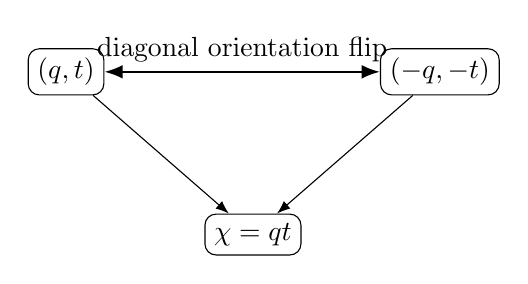
\begin{tikzpicture}[>=Latex,node distance=18mm]
\node (a) [draw,rounded corners] {$(q,t)$};
\node (b) [draw,rounded corners,right=35mm of a] {$(-q,-t)$};
\node (m) [draw,rounded corners,below=18mm of $(a)!0.5!(b)$] {$\chi=qt$};
\draw[<->,thick] (a)-- node[above]{diagonal orientation flip} (b);
\draw[->] (a)--(m); \draw[->] (b)--(m);
\end{tikzpicture}
\caption{The exact binary quotient. The two lifts differ upstairs but project to the same relational class downstairs. The signs $q$ and $t$ are individually convention-dependent; their product $\chi$ survives the diagonal reversal.}
\label{fig:quotient}
\end{figure}

\section{Two complex structures in standard charged-field theory}\label{sec:chargedkahler}
The relational-orientation programme has a nontrivial standard-field-theory precedent that is stronger than the elementary Wilson-line analogy. A charged K\"ahler space carries two commuting complex structures. To avoid collision with the electric-current symbol, write them as $I$ and $J$:
\begin{equation}
 I^2=J^2=-1,\qquad [I,J]=0.
\end{equation}
Their relative product is an involution,
\begin{equation}\label{eq:chargedKahlerQ}
 \boxed{Q=-IJ},\qquad Q^2=1.
\end{equation}
This construction is standard in the charged-field formalism reviewed by G\'erard and J\"akel~\cite{GerardJaekel2005}. It already contains the exact algebraic pattern ``two quarter-turn structures, one binary relative orientation.''

\begin{proposition}[Relative complex orientation]\label{prop:relativecomplex}
Let $I$ and $J$ commute and obey $I^2=J^2=-1$. Then $Q=-IJ$ is an involution. Simultaneous reversal of both complex orientations leaves $Q$ fixed,
\begin{equation}
 (-I,-J)\quad\Longrightarrow\quad Q'=-(-I)(-J)=Q,
\end{equation}
whereas reversal of either one alone sends $Q\mapsto-Q$.
\end{proposition}
\begin{proof}
Commutativity gives
\begin{equation}
 Q^2=(-IJ)(-IJ)=I^2J^2=1.
\end{equation}
The three reversal statements are immediate by substitution.
\end{proof}

For the charged Klein--Gordon system the relation becomes dynamical. Let $L$ denote the real first-order generator and $h=|L|$ its positive magnitude. In the standard charged K\"ahler construction one may write~\cite{GerardJaekel2005}
\begin{equation}\label{eq:Kahlerenergycomplex}
 I=J\frac{L}{|L|}.
\end{equation}
Using $J^2=-1$ and the compatibility assumptions of the construction,
\begin{equation}\label{eq:QsignL}
 \boxed{Q=-IJ=\frac{L}{|L|}},
 \qquad
 \boxed{L=Qh},
 \qquad h=|L|\ge0.
\end{equation}
Thus the underlying first-order frequency generator has two signs while the physical one-particle Hamiltonian is positive on both charge sectors.

\begin{theorem}[Signed frequency versus positive energy]\label{thm:signedfreqpositive}
In the two-sector normal form
\begin{equation}
 Q=\begin{pmatrix}1&0\\0&-1\end{pmatrix},\qquad
 h=\begin{pmatrix}\varepsilon&0\\0&\varepsilon\end{pmatrix},\qquad \varepsilon>0,
\end{equation}
we have
\begin{equation}
 L=Qh=\begin{pmatrix}\varepsilon&0\\0&-\varepsilon\end{pmatrix}.
\end{equation}
Hence opposite signs of the microscopic first-order generator coexist with the same positive physical energy $\varepsilon$.
\end{theorem}
\begin{proof}
Direct matrix multiplication gives the displayed $L$. The two eigenvectors of $Q$ have eigenvalues $\pm1$, while both are eigenvectors of $h$ with eigenvalue $\varepsilon$.
\end{proof}

This theorem sharply separates three notions that are often conflated: signed microscopic frequency, positive measured energy, and the thermodynamic arrow of a many-body observer. It also fixes the notation used throughout the orientation programme. The microscopic signs are
\begin{equation}\label{eq:gaugeTimeAlignmentDictionary}
 \begin{aligned}
 q&=\text{conjugate-representation orientation},\\
 t&=\text{time arrow, measured against the record arrow}.
 \end{aligned}
\end{equation}
with the observable charge/matter grading arising only from their relative alignment, $\chi=qt$. Neither sign should be identified naively with an already-measured scalar observable: $q$ labels which member of a conjugate representation pair is used relative to a reference convention, while $t$ labels the orientation of the first-order phase flow relative to the observer's chosen timelike orientation. Standard charged K\"ahler theory proves that such a relative-product mechanism is mathematically natural; it does not prove that these particular microscopic orientations are the fundamental structures of the Standard Model. The analogous dependence of fermionic quantization on a choice of complex structure is also standard in the spin-representation approach to the Dirac field~\cite{GraciaBondiaVarilly1994}, and the two-complex-structure interpretation of the negative-frequency/antiparticle split has been emphasized by Saunders~\cite{Saunders1991}.

\section{The spinor already has two lifts}
The proper orthochronous Lorentz group is covered twice by $\mathrm{SL}(2,\mathbb C)$. In the rotational subgroup,
\begin{equation}
 \mathrm{Spin}(3)\simeq SU(2)\longrightarrow SO(3),\qquad \ker=\{\pm1\}.
\end{equation}
A spinor rotated by angle $\theta$ about a unit vector $\hat n$ transforms as
\begin{equation}
 U(\theta)=\exp\!\left(-\frac{i\theta}{2}\hat n\cdot\bm\sigma\right).
\end{equation}
Therefore
\begin{equation}
 U(2\pi)=-1,\qquad U(4\pi)=+1.
\end{equation}
The half-angle, the sign after $2\pi$, and the $4\pi$ return are the same topological fact: vectors live on the quotient while spinors retain the lift. This is an exact source of a physically important factor $1/2$. It does not imply that every factor $1/2$ in physics has the same origin.

In this paragraph set $c=1$. For a future-pointing null momentum,
\begin{equation}
 p_{\alpha\dot\alpha}=\lambda_\alpha\bar\lambda_{\dot\alpha},
\end{equation}
so the spinor is literally a square root of the null vector up to phase. A timelike Hermitian momentum matrix of rank two requires two independent spinors,
\begin{equation}\label{eq:massivespinor}
 p_{\alpha\dot\alpha}=\lambda^I_\alpha\tilde\lambda_{\dot\alpha I},\qquad I=1,2,
\end{equation}
with
\begin{equation}
 \det p=p^2=m^2.
\end{equation}
Mass therefore appears precisely when a single null spinor square no longer suffices. This is kinematics, not yet an ontology of ``two universes.''

\section{Mass couples the chiral pair}
Fix the mostly-minus convention and $x^0=ct$. The free covariant Dirac equation is
\begin{equation}\label{eq:covariantDirac}
 \boxed{\left(i\hbar c\,\gamma^\mu\partial_\mu-mc^2\right)\psi=0.}
\end{equation}
In the Weyl basis it is equivalent to
\begin{align}
 i\hbar\partial_t\psi_L&=-i\hbar c\,\bm\sigma\cdot\nabla\psi_L+mc^2\psi_R,\\
 i\hbar\partial_t\psi_R&=+i\hbar c\,\bm\sigma\cdot\nabla\psi_R+mc^2\psi_L.
\end{align}
The massless equations decouple. At rest, coordinate time equals proper time, so writing the evolution parameter as $\tau$ makes the invariant clock explicit:
\begin{equation}\label{eq:rest}
 i\hbar\frac{d}{d\tau}
 \begin{pmatrix}\psi_L\\\psi_R\end{pmatrix}
 =mc^2\sigma_1
 \begin{pmatrix}\psi_L\\\psi_R\end{pmatrix}.
\end{equation}
Write $\omega_C=mc^2/\hbar$. Then
\begin{equation}\label{eq:Ut}
 U(\tau)=e^{-i\omega_C\tau\sigma_1}
 =\cos(\omega_C\tau)\,1-i\sin(\omega_C\tau)\,\sigma_1.
\end{equation}
If $|L\rangle=(1,0)^T$ and $|R\rangle=(0,1)^T$, Eq.~\eqref{eq:Ut} gives
\begin{equation}\label{eq:chiralevol}
 |L;\tau\rangle=\cos(\omega_C\tau)|L\rangle-i\sin(\omega_C\tau)|R\rangle,
\end{equation}
and therefore
\begin{equation}\label{eq:pop}
 P_R(\tau)=\sin^2(\omega_C\tau)=\frac{1-\cos(2\omega_C\tau)}2.
\end{equation}
Thus the population oscillation has angular frequency
\begin{equation}\label{eq:lock}
 \boxed{\omega_Z=2\omega_C=\frac{2mc^2}{\hbar}}.
\end{equation}
The factor two is not inserted by interpretation; it is the identity $\sin^2x=(1-\cos2x)/2$ applied to the spin-$1/2$ evolution generated by the mass term.

\begin{theorem}[Dirac half-angle and Hadamard bridge]\label{thm:hadamard}
At rest, the energy eigenstates of the Dirac Hamiltonian in chirality space are the $\sigma_1$ eigenstates
\begin{equation}
 |+\rangle=\frac{|L\rangle+|R\rangle}{\sqrt2},\qquad
 |-\rangle=\frac{|L\rangle-|R\rangle}{\sqrt2},
\end{equation}
with energies $\pm mc^2$. Conversely,
\begin{equation}\label{eq:hadamard}
 |L\rangle=\frac{|+\rangle+|-\rangle}{\sqrt2},\qquad
 |R\rangle=\frac{|+\rangle-|-\rangle}{\sqrt2}.
\end{equation}
Hence a sharp chiral state necessarily contains equal positive- and negative-frequency amplitudes, and the coefficient $1/\sqrt2$ is forced by normalization of the two-component decomposition.
\end{theorem}
\begin{proof}
Equation~\eqref{eq:rest} has Hamiltonian $H=mc^2\sigma_1$. Diagonalizing $\sigma_1$ gives the stated normalized eigenvectors. Inverting the resulting $2\times2$ orthogonal matrix gives Eq.~\eqref{eq:hadamard}.
\end{proof}

There is also an exact phase hierarchy. At
\begin{equation}
 \tau=\frac{\pi}{2\omega_C},\qquad |L\rangle\mapsto-i|R\rangle,
\end{equation}
so one chiral exchange occurs. At $\tau=\pi/\omega_C$ the chiral population has completed a full cycle while the spinor has acquired the sign $-1$. Only at $\tau=2\pi/\omega_C$ does the spinor itself return. The same two-cover logic that distinguishes a vector's $2\pi$ return from a spinor's $4\pi$ return is therefore mirrored dynamically by the rest-frame chiral clock. This is an isomorphism of the two-state evolution, not yet a proof that spatial spin rotation and chirality exchange are the same physical motion.

The invariant rest action is
\begin{equation}
 S=-mc^2\int d\tau,
\end{equation}
and hence the quantum phase advances as
\begin{equation}\label{eq:propertime}
 \varphi(\tau)=-\frac{mc^2}{\hbar}\tau=-\omega_C\tau.
\end{equation}
Mass is therefore the conversion factor between proper time and quantum phase. In the null limit there is no timelike rest frame and no corresponding rest-frame proper-time clock; this is sharper than saying that a massless particle carries a ``stopped'' clock.

\begin{proposition}[Mass is the free Dirac scale]\label{prop:scale}
In natural units and four spacetime dimensions, the massless Dirac action
\begin{equation}
 S_0=\int d^4x\,i\bar\psi\gamma^\mu\partial_\mu\psi
\end{equation}
is classically invariant under $x\mapsto\lambda x$, $\psi(x)\mapsto\lambda^{-3/2}\psi(\lambda^{-1}x)$. The mass term
\begin{equation}
 S_m=-\int d^4x\,m\bar\psi\psi
\end{equation}
introduces a dimension-one parameter and breaks this scale invariance unless $m$ is transformed spurionically as $m\mapsto\lambda^{-1}m$.
\end{proposition}
The same parameter therefore produces both the intrinsic clock $\omega_C^{-1}$ and the intrinsic ruler $\bar\lambda_C$. Their product is fixed by the conversion speed $c$ rather than by a new dimensionless constant.

\begin{figure}[t]
\centering
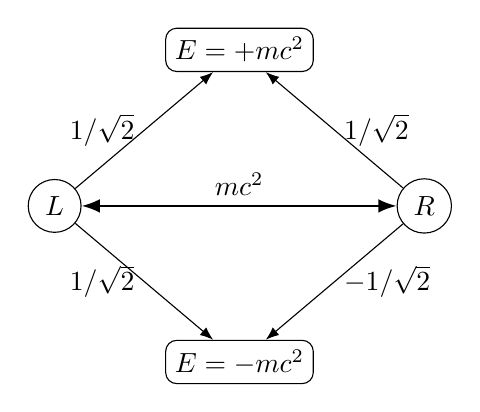
\begin{tikzpicture}[>=Latex,node distance=17mm]
\node (L) [draw,circle] {$L$};
\node (R) [draw,circle,right=40mm of L] {$R$};
\node (P) [draw,rounded corners,above=17mm of $(L)!0.5!(R)$] {$E=+mc^2$};
\node (M) [draw,rounded corners,below=17mm of $(L)!0.5!(R)$] {$E=-mc^2$};
\draw[<->,thick] (L)-- node[above] {$mc^2$} (R);
\draw[->] (L)-- node[left] {$1/\sqrt2$} (P);
\draw[->] (R)-- node[right] {$1/\sqrt2$} (P);
\draw[->] (L)-- node[left] {$1/\sqrt2$} (M);
\draw[->] (R)-- node[right] {$-1/\sqrt2$} (M);
\end{tikzpicture}
\caption{At rest, mass is the off-diagonal coupling of the chiral basis. Diagonalizing it produces the positive/negative-energy basis, with the exact $1/\sqrt2$ coefficients of the Hadamard transform.}
\label{fig:hadamard}
\end{figure}


\section{Mass as invariant phase density: the exact time--length bridge}
The relation between mass, proper time and the speed $c$ can be stated without interpretation. Let a freely propagating massive degree of freedom have Hamilton principal function $S$. In geometric units one often writes $S=-m\int ds$; with $ds=c\,d\tau$ and conventional units restored,
\begin{equation}\label{eq:massaction}
 S=-mc^2\int d\tau=-mc\int ds.
\end{equation}
Define the dimensionless quantum phase
\begin{equation}\label{eq:theta}
 \theta=\frac{S}{\hbar}.
\end{equation}
Use the phase convention $\psi\sim e^{iS/\hbar}$. A positive-frequency plane wave has $S=-p\cdot x$, so the physical future-directed momentum is
\begin{equation}\label{eq:HJmomentumsign}
 p_\mu=-\partial_\mu S.
\end{equation}
The sign disappears from the Hamilton--Jacobi mass shell,
\begin{equation}\label{eq:HJmass}
 g^{\mu\nu}\partial_\mu S\,\partial_\nu S=m^2c^2,
\end{equation}
for the mostly-minus convention. Dividing by $\hbar^2$ gives an invariant statement about the phase gradient.

\begin{theorem}[Mass--phase geometry]\label{thm:massphase}
For a free massive relativistic mode with phase $\theta=S/\hbar$,
\begin{equation}\label{eq:phasegradient}
 p_\mu=-\hbar\,\partial_\mu\theta,
 \qquad
 g^{\mu\nu}\partial_\mu\theta\,\partial_\nu\theta
 =\left(\frac{mc}{\hbar}\right)^2
 =\frac{1}{\bar\lambda_C^2},
\end{equation}
where $\bar\lambda_C=\hbar/(mc)$. Along the particle proper time,
\begin{equation}\label{eq:phaserate}
 \frac{d\theta}{d\tau}=-\frac{mc^2}{\hbar}=-\omega_C,
 \qquad
 \frac{d\theta}{ds}=-\frac{mc}{\hbar}=-\frac1{\bar\lambda_C}.
\end{equation}
Consequently
\begin{equation}\label{eq:massclockbridge}
 \boxed{\omega_C=\frac{c}{\bar\lambda_C}},
 \qquad
 \boxed{m=\frac{\hbar}{c^2}\left|\frac{d\theta}{d\tau}\right|}
 =\frac{\hbar}{c}\left|\frac{d\theta}{ds}\right|.
\end{equation}
Thus mass is exactly the Lorentz-invariant phase density per unit proper time, equivalently per unit proper length; $c$ is the conversion between those two descriptions.
\end{theorem}
\begin{proof}
The first identity follows from the stated positive-frequency phase convention $\psi\sim e^{iS/\hbar}$ and Eq.~\eqref{eq:HJmomentumsign}. The mass-shell condition $p^2=m^2c^2$ gives Eq.~\eqref{eq:phasegradient}. Differentiating Eq.~\eqref{eq:massaction} along proper time gives $dS/d\tau=-mc^2$, hence Eq.~\eqref{eq:phaserate}. Since $ds=c\,d\tau$, the remaining identities follow algebraically.
\end{proof}

This theorem is the precise content behind the phrase ``mass is a clock.'' It is stronger and less anthropomorphic: mass does not merely correlate with a frequency; it is the invariant norm of the phase gradient, while proper time is the parameter with respect to which that phase accumulates at the scalar rate $mc^2/\hbar$. The same invariant determines a ruler and a clock,
\begin{equation}
 \kappa_C\equiv\frac1{\bar\lambda_C}=\frac{mc}{\hbar},
 \qquad
 \omega_C=c\kappa_C.
\end{equation}
No additional dimensionless constant is required. The null limit $m\to0$ simultaneously removes the rest-frame phase rate and sends the intrinsic Compton length to infinity; this is why the massive and massless sectors differ qualitatively rather than merely quantitatively.

\subsection{Orientation reversal dualizes the proper-time character}
There is a second exact statement. Proper-time translations carry the one-dimensional unitary character
\begin{equation}\label{eq:timecharacter}
 \chi_m(\tau)=e^{-i\omega_C\tau}.
\end{equation}
Reversing the orientation of the parameter gives
\begin{equation}\label{eq:timecharacterdual}
 \chi_m(-\tau)=e^{+i\omega_C\tau}=\chi_m(\tau)^*=\chi_m(\tau)^{-1}.
\end{equation}
This is the same representation-theoretic operation that appeared for an Abelian Wilson line: reversal of an oriented one-dimensional path sends a unitary character to its dual.

\begin{proposition}[Universal character--orientation duality]\label{prop:characterduality}
Let $\chi$ be any one-dimensional unitary representation evaluated on an oriented one-parameter path. Path reversal sends
\begin{equation}
 \chi\longmapsto\chi^{-1}=\chi^*.
\end{equation}
For electromagnetic transport the representation label is charge $q$; for proper-time translations it is the frequency $E/\hbar$. Thus the charge-conjugate Wilson phase and the opposite-frequency proper-time phase are two exact realizations of the same dualization functor on one-dimensional unitary representations.
\end{proposition}
\begin{proof}
A one-dimensional unitary representation has values in $U(1)$. Reversal replaces the group parameter $a$ by $-a$, so $\chi(-a)=\chi(a)^{-1}$. Unitarity gives $\chi(a)^{-1}=\chi(a)^*$.
\end{proof}

This proposition does \emph{not} identify electric charge with energy or Wigner time reversal with charge conjugation. It isolates the common mathematics: orientation reversal acts by dualization on both character lines. The stronger Shadow proposal is that the relevant character lines are associated to one physical orientation lift; that identification still requires an intertwiner.

\subsection{The factor two is an exact \texorpdfstring{$SU(2)\to SO(3)$}{SU(2) to SO(3)} projective clock}
The rest-frame Dirac system of Eq.~\eqref{eq:rest} has
\begin{equation}
 U(t)=e^{-i\omega_Ct\sigma_1}.
\end{equation}
A normalized two-component state defines a Bloch vector $\bm n=\langle\bm\sigma\rangle$. The physical bilinears transform by conjugation, not by the fundamental spinor matrix itself.

\begin{theorem}[Projective Compton clock]\label{thm:projectiveclock}
Under $U(t)=e^{-i\omega_Ct\sigma_1}$ the Bloch vector rotates about the $1$-axis through angle
\begin{equation}\label{eq:blochangle}
 \Theta(t)=2\omega_Ct.
\end{equation}
Equivalently,
\begin{align}
 U(t)^\dagger\sigma_3U(t)&=\sigma_3\cos(2\omega_Ct)-\sigma_2\sin(2\omega_Ct),\\
 U(t)^\dagger\sigma_2U(t)&=\sigma_2\cos(2\omega_Ct)+\sigma_3\sin(2\omega_Ct).
\end{align}
Therefore every projective/bilinear observable returns after $t=\pi/\omega_C$, at which time
\begin{equation}\label{eq:deckclock}
 U\!\left(\frac{\pi}{\omega_C}\right)=-1,
\end{equation}
while the spinor itself returns only after $t=2\pi/\omega_C$. The frequency doubling $\omega_Z=2\omega_C$ is therefore exactly the fundamental-versus-adjoint double-cover factor of this internal $SU(2)$ evolution.
\end{theorem}
\begin{proof}
The Pauli commutation relations give the standard adjoint action of $SU(2)$ on its Lie algebra. Since the fundamental element is $e^{-i(\Theta/2)\sigma_1}$, comparison with $e^{-i\omega_Ct\sigma_1}$ gives $\Theta=2\omega_Ct$. At $t=\pi/\omega_C$ the fundamental matrix is $e^{-i\pi\sigma_1}=-1$, whose adjoint action is the identity; at twice that time the fundamental matrix itself is $+1$.
\end{proof}

This theorem materially strengthens the earlier observation that $\sin^2(\omega_Ct)$ contains $2\omega_C$. The factor two is not merely trigonometric: it is the defining half-angle relation between a two-component spinor and its projective observables. The internal Bloch sphere is not automatically the physical spatial rotation group, so this does not yet prove that zitterbewegung \emph{causes} spacetime spin $1/2$. It does, however, establish an exact double-cover dynamical mechanism at the Compton scale. Any proposed temporal-lift/spin intertwiner must reproduce this theorem rather than merely resemble it.

\section{The reciprocal Compton pair}
For the free Dirac Hamiltonian
\begin{equation}
 H=c\bm\alpha\cdot\bm p+\beta mc^2,
\end{equation}
the Heisenberg equation gives
\begin{equation}
 \dot\alpha_i=\frac{i}{\hbar}[H,\alpha_i]
 =\frac{2i}{\hbar}(c p_i-H\alpha_i).
\end{equation}
Solving,
\begin{equation}\label{eq:alphaH}
 \alpha_i(t)=c p_iH^{-1}+\left(\alpha_i(0)-c p_iH^{-1}\right)e^{-2iHt/\hbar},
\end{equation}
and integrating $\dot x_i=c\alpha_i$ yields
\begin{equation}\label{eq:xH}
 x_i(t)=x_i(0)+c^2p_iH^{-1}t+\frac{i\hbar c}{2}H^{-1}
 \left(\alpha_i(0)-c p_iH^{-1}\right)\left(e^{-2iHt/\hbar}-1\right).
\end{equation}
The oscillatory term therefore carries the exact phase $2Ht/\hbar$. At rest, $H^2=m^2c^4$, so the angular frequency is $2mc^2/\hbar$ and the natural displacement scale is $\hbar/(2mc)$. This is the operator-level origin of the same factor two found in the chiral population. The characteristic zitterbewegung amplitude is
\begin{equation}
 a_Z=\frac{\hbar}{2mc}=\frac{\bar\lambda_C}{2},
 \qquad
 \bar\lambda_C=\frac{\hbar}{mc}.
\end{equation}
Together with Eq.~\eqref{eq:lock},
\begin{equation}\label{eq:azwz}
 \boxed{a_Z\omega_Z=c}.
\end{equation}
The ordinary reduced Compton scales satisfy
\begin{equation}\label{eq:comptonpair}
 \boxed{\bar\lambda_C\omega_C=c}.
\end{equation}
Thus the Dirac internal motion replaces $(\bar\lambda_C,\omega_C)$ by the reciprocal pair $(\bar\lambda_C/2,2\omega_C)$ without changing their product. This is a precise instance in which the recurring $1/2$ and $2$ are the two faces of one representation-theoretic scaling.

\begin{proposition}[No numerological inference]\label{prop:numerology}
Equations~\eqref{eq:lock}--\eqref{eq:comptonpair} justify grouping the factors $2$ and $1/2$ that arise from the same Dirac/spinor structure. They do not justify assigning a common origin to unrelated normalization factors such as the $1/\sqrt2$ in a normalized null basis $x^\pm=(t\pm x)/\sqrt2$.
\end{proposition}

\section{Locality does not select one frequency sign}
The positive-energy projector of the free Dirac Hamiltonian is
\begin{equation}
 P_+(\bm p)=\frac12\left(1+\frac{c\bm\alpha\cdot\bm p+\beta mc^2}{\sqrt{c^2\bm p^2+m^2c^4}}\right).
\end{equation}
Because of the square-root dispersion, its position-space kernel is nonlocal and has a characteristic Compton scale. A strictly local multiplication operator is therefore not, in general, diagonal in the positive/negative-energy splitting. This gives a conservative meaning to the statement that a local massive fermionic probe addresses the full Dirac structure rather than a globally isolated frequency sign.

It does \emph{not} follow from the projector calculation alone that a real electron literally reverses its coordinate-time orientation every Compton period. The two frequency sectors are present in the local relativistic field description itself. The stronger possibility that their interference is the quantum trace of a microscopic temporal-orientation switchback is therefore stated separately and given a falsification condition below.


\section{One time axis, two microscopic orientations, and the four-lift carrier}\label{sec:fourlift}
The temporal sign used in this paper is not a second time coordinate. Let $u^\mu$ be a unit timelike vector defining the local time orientation of an observer, and let a massive microscopic phase $\varphi$ have covector $k_\mu=\nabla_\mu\varphi$. Whenever $k$ is timelike relative to the same local metric, define the observer-relative phase orientation
\begin{equation}\label{eq:tphasecovariant}
 \boxed{t_u(k)=\sgn\!\bigl(-u^\mu k_\mu\bigr)\in\{+1,-1\}.}
\end{equation}
Changing the observer's time orientation $u\mapsto-u$ reverses $t_u(k)$ without introducing a new temporal dimension. Equivalently, if $d\tau\ge0$ denotes the unsigned proper-time length along a timelike line, an oriented proper-time element may be written
\begin{equation}\label{eq:orientedpropertime}
 d\tau_{\rm or}=t\,d\tau,\qquad t=\pm1.
\end{equation}
The Compton character then reads
\begin{equation}\label{eq:orientedComptonphase}
 d\varphi=-\omega_C\,d\tau_{\rm or}
 =-t\,\frac{mc^2}{\hbar}\,d\tau.
\end{equation}
Thus the microscopic arrow is an orientation of the same proper-time line used by macroscopic matter, not an additional coordinate.

The second sign is the orientation $q=\pm1$ of a conjugate gauge/charge representation relative to a chosen charge standard. The exact oriented-line calculation of Section~2 then singles out the relational grading
\begin{equation}\label{eq:chiqt4}
 \boxed{\chi=qt.}
\end{equation}
Only the alignment is invariant under simultaneous reversal. This is the minimal algebra behind the statement ``particle identity is relational.''

To state the finite quantum version, introduce four kinematic lifts
\begin{equation}\label{eq:fourlifts}
 |++\rangle,\quad |+-\rangle,\quad |-+\rangle,\quad |--\rangle,
\end{equation}
where the first sign is $q$ and the second is $t$. On the carrier $\widetilde{\mathcal H}_{\rm or}\simeq\mathbb C^4$ define
\begin{equation}\label{eq:IqIt}
 I_q=i\,\mathrm{diag}(1,1,-1,-1),\qquad
 I_t=i\,\mathrm{diag}(1,-1,1,-1).
\end{equation}
Then
\begin{equation}
 I_q^2=I_t^2=-1,\qquad [I_q,I_t]=0,
\end{equation}
and
\begin{equation}\label{eq:chiIqIt}
 \boxed{\chi=-I_qI_t=\mathrm{diag}(1,-1,-1,1)}.
\end{equation}
Thus the aligned lifts $++$ and $--$ carry $\chi=+1$, while the anti-aligned lifts $+-$ and $-+$ carry $\chi=-1$.

To avoid collision with the later Grassmannian determinant $D=\det A$, write the simultaneous reversal operator as $\mathsf D$:
\begin{equation}\label{eq:Ddef}
 \mathsf D|++\rangle=|--\rangle,\quad \mathsf D|--\rangle=|++\rangle,\quad
 \mathsf D|+-\rangle=|-+\rangle,\quad \mathsf D|-+\rangle=|+-\rangle.
\end{equation}

\begin{theorem}[Diagonal-reversal algebra]\label{thm:diagonalcover}
The operators in Eqs.~\eqref{eq:IqIt}--\eqref{eq:Ddef} satisfy
\begin{equation}\label{eq:Danti}
 \mathsf D I_q=-I_q\mathsf D,\qquad
 \mathsf D I_t=-I_t\mathsf D,
\end{equation}
while
\begin{equation}\label{eq:Dchi}
 [\mathsf D,\chi]=0.
\end{equation}
Equivalently,
\begin{equation}\label{eq:ItIqchi}
 \boxed{I_t=I_q\chi.}
\end{equation}
Thus each microscopic complex orientation is reversed by $\mathsf D$, whereas their relative orientation is preserved.
\end{theorem}
\begin{proof}
The first three identities follow by direct action on the four basis states. Equation~\eqref{eq:ItIqchi} follows from $\chi=-I_qI_t$ and $I_q^2=-1$.
\end{proof}

The operator algebra is already more rigid than the four labels alone suggest. The labels form the Klein four-group, but the quarter-turn operators do not.

\begin{theorem}[Finite carrier group and center]\label{thm:orientationgroup}
Let
\begin{equation}
 \mathcal G_{qt}:=\langle I_q,I_t,\mathsf D\rangle
 \subset GL_{\mathbb C}(\widetilde{\mathcal H}_{\rm or}).
\end{equation}
Then $|\mathcal G_{qt}|=16$ and
\begin{equation}\label{eq:orientationgroupiso}
 \boxed{
 \mathcal G_{qt}\simeq
 (\text{dihedral group of order }8)\times\mathbb Z_2.}
\end{equation}
Its center is
\begin{equation}\label{eq:orientationcenter}
 \boxed{Z(\mathcal G_{qt})=\{1,-1,\chi,-\chi\}\simeq\mathbb Z_2\times\mathbb Z_2.}
\end{equation}
In particular $\chi$ is central, while $\mathsf D$ is not.
\end{theorem}
\begin{proof}
The subgroup $H=\langle I_q,\mathsf D\rangle$ obeys
\begin{equation}
 I_q^4=1,\qquad \mathsf D^2=1,\qquad
 \mathsf D I_q\mathsf D=I_q^{-1},
\end{equation}
so the explicit matrices generate the dihedral group of order eight. Equation~\eqref{eq:ItIqchi} gives $I_t=I_q\chi$. The involution $\chi$ commutes with both $I_q$ and $\mathsf D$ and is not an element of $H$, so $\mathcal G_{qt}=H\times\langle\chi\rangle$. The center of $H$ is $\{1,I_q^2\}=\{1,-1\}$; multiplying by $\{1,\chi\}$ gives Eq.~\eqref{eq:orientationcenter}.
\end{proof}

This immediately separates two order-two operations that earlier versions risked conflating. The scalar $-1=I_q^2=I_t^2$ is central, whereas $\mathsf D$ is noncentral because it anticommutes with $I_q$. Hence
\begin{equation}\label{eq:DnotminusI}
 \boxed{\mathsf D\neq-1,\qquad \mathsf D\text{ and }-1\text{ lie in different conjugacy classes}.}
\end{equation}
Indeed no automorphism of $\mathcal G_{qt}$ can exchange them because automorphisms preserve the center. This distinction will matter when the Compton half-period is compared with the orientation involution: the Dirac half-period produces the central scalar $-1$, not $\mathsf D$.

\subsection{The diagonal reversal is a real structure, not a third gauge phase}\label{subsec:Drealform}
The carrier $\mathbb C^4$ has its ordinary quantum-mechanical scalar $i$, but $I_q$ itself also defines a complex structure on the underlying real vector space. Relative to that complex structure, Eq.~\eqref{eq:Danti} says precisely that $\mathsf D$ is anti-linear:
\begin{equation}\label{eq:DantilinearIq}
 \boxed{\mathsf D(I_qv)=-I_q(\mathsf Dv),\qquad \mathsf D^2=1.}
\end{equation}
Thus $\mathsf D$ is a real structure on $(\widetilde{\mathcal H}_{\rm or},I_q)$.

Its fixed set is
\begin{equation}\label{eq:VDfixed}
 \mathcal H_{\mathsf D}
 :=\operatorname{Fix}(\mathsf D)
 =\{(a,b,b,a):a,b\in\mathbb C\}.
\end{equation}
This space has complex dimension two with respect to the ordinary ambient scalar $i$, hence real dimension four. Relative to the microscopic complex structure $I_q$, however, it is a real form:
\begin{equation}\label{eq:realformdecomp}
 \boxed{
 \widetilde{\mathcal H}_{\rm or}
 =\mathcal H_{\mathsf D}\oplus I_q\mathcal H_{\mathsf D}
 \quad\text{as real vector spaces}.}
\end{equation}
Moreover $I_q\mathcal H_{\mathsf D}$ is exactly the $\mathsf D$-odd subspace.

\begin{theorem}[Real-form projection]\label{thm:Drealform}
The operator
\begin{equation}\label{eq:PD}
 P_{\mathsf D}:=\frac{1+\mathsf D}{2}
\end{equation}
is the idempotent projection onto $\mathcal H_{\mathsf D}$. Its formula is numerically the same as an average over an order-two linear action, but its physical role here is the real-part projection associated with the anti-linear structure of Eq.~\eqref{eq:DantilinearIq}; no finite gauge group need be postulated.
\end{theorem}
\begin{proof}
Since $\mathsf D^2=1$,
\begin{equation}
 P_{\mathsf D}^2=\frac{1+2\mathsf D+\mathsf D^2}{4}=P_{\mathsf D}.
\end{equation}
Its image is fixed by $\mathsf D$, and every fixed vector is left unchanged. The real-form statement follows from the decomposition into $\mathsf D$-even and $\mathsf D$-odd parts together with Eq.~\eqref{eq:Danti}.
\end{proof}

This corrects the interpretation of the same formula in earlier versions. The finite Haar calculation on the four \emph{labels} remains a valid representation-theoretic identity: averaging functions on the Klein four-group over the diagonal label flip keeps only the trivial and $\chi$ characters. What no longer follows is that the Hilbert-space carrier itself should be interpreted as a finite gauge average. The physical proposal is instead the $I_q$-real form $\mathcal H_{\mathsf D}$.

\subsection{Exact identification with the charged-K\"ahler two-sector normal form}
The preceding construction and Section~\ref{sec:chargedkahler} are not merely analogous finite algebras. They are explicitly intertwined. Define
\begin{equation}\label{eq:PhiKahler}
 \Phi:\mathcal H_{\mathsf D}\longrightarrow\mathbb C^2,
 \qquad
 \Phi(a,b,b,a)=(a,b).
\end{equation}
Then
\begin{equation}\label{eq:PhiChiQ}
 \boxed{
 \Phi\,\chi\,\Phi^{-1}
 =\begin{pmatrix}1&0\\0&-1\end{pmatrix}=Q.}
\end{equation}
Together with $I_t=I_q\chi$, this is the same multiplication law as the charged-K\"ahler identity $J=IQ$ or, equivalently, $Q=-IJ$.

\begin{theorem}[Four-lift/charged-K\"ahler intertwiner]\label{thm:Kahlerfourlift}
Under the map $\Phi$, the relational grading $\chi$ on the $\mathsf D$-real carrier is exactly the standard two-sector charge involution $Q$. Consequently the finite orientation carrier and the charged-K\"ahler normal form contain one and the same relative-complex-orientation algebra. What remains a physical hypothesis is the identification of the microscopic geometric structures represented by $I_q$ and $I_t$ with the corresponding structures of the interacting charged field.
\end{theorem}
\begin{proof}
From Eq.~\eqref{eq:VDfixed},
\begin{equation}
 \chi(a,b,b,a)=(a,-b,-b,a).
\end{equation}
Applying $\Phi$ gives $(a,-b)$, which is Eq.~\eqref{eq:PhiChiQ}.
\end{proof}

The natural normalized charge eigenvectors are therefore still
\begin{equation}\label{eq:Mstates}
 |e^-\rangle_{\rm or}=\frac{|++\rangle+|--\rangle}{\sqrt2},\qquad
 |e^+\rangle_{\rm or}=\frac{|+-\rangle+|-+\rangle}{\sqrt2},
\end{equation}
with
\begin{equation}
 \chi|e^-\rangle_{\rm or}=+|e^-\rangle_{\rm or},\qquad
 \chi|e^+\rangle_{\rm or}=-|e^+\rangle_{\rm or}.
\end{equation}
The equal amplitudes inside each pair are now read as the fixed-real-form condition, not as evidence that a physical electron is a classical statistical mixture of two hidden species.


\subsection{The full carrier has a split-Clifford realization}\label{subsec:Dsignature}
Section~\ref{subsec:Drealform} determines the abstract operator algebra without yet deriving it from a quadratic space. To ask for a minimal Clifford origin, impose one additional and explicit hypothesis: represent $I_q$, $I_t$ and $\mathsf D$ by nonproportional simple bivectors in a real rank-four Clifford algebra. Under this hypothesis the signature is forced, and the resulting spin module reproduces the four-lift matrices exactly.

\begin{theorem}[Minimal simple-bivector signature]\label{thm:Dsignature}
Let $V$ be a nondegenerate real quadratic space of dimension four and signature $(p,q)$. Suppose nonzero bivectors $a,b,c\in\Lambda^2V\subset\mathrm{Cl}(V)$ satisfy
\begin{equation}\label{eq:Dsigrelations}
 a^2=b^2=-1,\qquad [a,b]=0,\qquad a\neq\pm b,
 \qquad c^2=+1,\qquad \{c,a\}=\{c,b\}=0.
\end{equation}
Then $(p,q)=(2,2)$. Conversely, in an orthonormal basis with
$e_1^2=e_2^2=+1$ and $e_3^2=e_4^2=-1$, the normal form
\begin{equation}\label{eq:Dsigsolution}
 \boxed{a=e_1e_2,\qquad b=e_3e_4,\qquad c=e_2e_4}
\end{equation}
satisfies Eq.~\eqref{eq:Dsigrelations}.
\end{theorem}

\begin{proof}
For a bivector $B$ in four dimensions, the grade-four part of $B^2$ is $B\wedge B$. Since each square in Eq.~\eqref{eq:Dsigrelations} is scalar, $B\wedge B=0$ for $B=a,b,c$; the four-dimensional Pl\"ucker relation therefore makes each bivector decomposable. Their nonzero scalar squares make the associated two-planes nondegenerate.

Let $A\subset V$ be the plane of $a$. Decompose
\begin{equation}
 \Lambda^2V=\Lambda^2A\oplus(A\wedge A^\perp)\oplus\Lambda^2A^\perp.
\end{equation}
The commutator with the nondegenerate plane element $a$ is invertible on the mixed summand and vanishes on the two pure summands. Hence a bivector commuting with $a$ lies in $\Lambda^2A\oplus\Lambda^2A^\perp$. A decomposable element with components in both one-dimensional summands would have nonzero wedge square. Since $b\neq\pm a$, the plane of $b$ is therefore $A^\perp$.

The signs $a^2=b^2=-1$ say that both orthogonal planes are definite. Anticommutation with both $a$ and $b$ places $c$ in the mixed summand $A\wedge A^\perp$. Decomposability makes $c=u\wedge w$ with $u\in A$ and $w\in A^\perp$. Finally $c^2=+1$ says that $u$ and $w$ have opposite metric signs. Thus the two definite planes have opposite signs and $V$ has signature $(2,2)$. The converse follows directly from $(e_ie_j)^2=-e_i^2e_j^2$ and the parity of the required reorderings.
\end{proof}

The qualification ``simple-bivector'' is essential. The abstract finite algebra can be embedded in larger matrix or Clifford algebras in many ways; the theorem classifies its minimal rank-four geometric realization, not every possible representation.

\begin{theorem}[Explicit Clifford intertwiner]\label{thm:explicitCl22carrier}
Let
\begin{equation}
 X=\begin{pmatrix}0&1\\1&0\end{pmatrix},\qquad
 Z=\begin{pmatrix}1&0\\0&-1\end{pmatrix},\qquad
 J=\begin{pmatrix}0&1\\-1&0\end{pmatrix},
\end{equation}
and define a real representation of $\mathrm{Cl}(2,2)\simeq M_4(\mathbb R)$ by
\begin{equation}\label{eq:Cl22gammas}
 \Gamma_1=X\otimes1,\quad \Gamma_2=Z\otimes1,
 \quad \Gamma_3=J\otimes X,\quad \Gamma_4=J\otimes Z.
\end{equation}
Set
\begin{equation}\label{eq:Cl22orientationops}
 a=\Gamma_1\Gamma_2,\quad b=\Gamma_3\Gamma_4,
 \quad c=\Gamma_2\Gamma_4,
 \quad r_q=\Gamma_1,
 \quad r_t=\Gamma_1\Gamma_2\Gamma_4=r_qc.
\end{equation}
After complexification there is a unitary basis $|q,t\rangle$, $q,t=\pm1$, in which
\begin{equation}\label{eq:Cl22intertwining}
 a=I_q,\qquad b=I_t,\qquad c=\mathsf D,\qquad
 r_q=R_q,\qquad r_t=R_t.
\end{equation}
Moreover
\begin{equation}\label{eq:chiCl22volume}
 \boxed{\chi=-ab=-\Gamma_1\Gamma_2\Gamma_3\Gamma_4,}
\end{equation}
so the relational grading is the negative split volume element.
\end{theorem}

\begin{proof}
The matrices in Eq.~\eqref{eq:Cl22gammas} anticommute and square respectively to $+1,+1,-1,-1$. Equations~\eqref{eq:Dsigrelations} and the half-flip relations follow by Clifford multiplication. In particular
\begin{equation}
 r_qr_t=c,\qquad r_q^2=r_t^2=1,\qquad
 r_q a=-a r_q,\quad [r_q,b]=0,\qquad
 [r_t,a]=0,\quad r_tb=-br_t.
\end{equation}
For an explicit simultaneous eigenbasis, put
\begin{equation}
 u_q=2^{-1/2}\binom{1}{-iq},\qquad
 w_t=2^{-1/2}\binom{1}{it},\qquad
 \alpha_+=1,\quad\alpha_-=-i,
\end{equation}
and set $|q,t\rangle=\alpha_q\,u_q\otimes w_t$. Then
\begin{equation}
 a|q,t\rangle=iq|q,t\rangle,\qquad
 b|q,t\rangle=it|q,t\rangle,\qquad
 c|q,t\rangle=|-q,-t\rangle,
\end{equation}
while $r_q$ and $r_t$ flip only their indicated signs. This is exactly Eqs.~\eqref{eq:IqIt}, \eqref{eq:Ddef} and the definitions of $R_q,R_t$. Finally Eq.~\eqref{eq:chiCl22volume} follows from $\chi=-ab$.
\end{proof}

Equation~\eqref{eq:chiCl22volume} explains the centrality of $\chi$ without making it automatically observable: the volume element is central in the even split-Clifford algebra, while the odd half flips reverse it. Indeed
\begin{equation}
 \mathrm{Cl}^0(2,2)\simeq M_2(\mathbb R)\oplus M_2(\mathbb R),
\end{equation}
and the two summands are the $\chi=\pm1$ chiral sectors. The extra real structure is the even element $c$, not the central volume element and not the scalar $-1$.

\begin{corollary}[Exact origin of the half-flip identity]\label{cor:Cl22halfflip}
Since $r_t=r_qc$, one has
\begin{equation}
 \boxed{r_t v=r_qv\quad\text{for every }v\in\operatorname{Fix}(c).}
\end{equation}
Thus Corollary~\ref{cor:halfflipidentity} is the restriction of an exact Clifford identity, not a coincidence of two permutation matrices.
\end{corollary}

Theorem~\ref{thm:Dsignature} classifies the simple-bivector geometry. Dropping that hypothesis changes the answer in exactly one signature, and the change matters for how the result may be used.

\begin{theorem}[All rank-four realizations]\label{thm:Dsignaturegeneral}
Let $p+q=4$. There exist elements $a,b,c\in\mathrm{Cl}(p,q)$, not required to be bivectors, satisfying Eq.~\eqref{eq:Dsigrelations} if and only if $\mathrm{Cl}(p,q)\simeq M_4(\mathbb R)$, that is,
\begin{equation}\label{eq:Dsiggeneral}
 \boxed{(p,q)\in\{(2,2),\,(3,1)\}.}
\end{equation}
\end{theorem}
\begin{proof}
The rank-four real Clifford algebras are $\mathrm{Cl}(2,2)\simeq\mathrm{Cl}(3,1)\simeq M_4(\mathbb R)$ and $\mathrm{Cl}(4,0)\simeq\mathrm{Cl}(1,3)\simeq\mathrm{Cl}(0,4)\simeq M_2(\mathbb H)$.

If $\mathrm{Cl}(p,q)\simeq M_4(\mathbb R)$, the matrices of Theorem~\ref{thm:explicitCl22carrier} lie in it. For $(3,1)$ this is explicit: the real matrices
\begin{equation}
 \Gamma'_1=X\otimes1,\quad \Gamma'_2=Z\otimes1,\quad \Gamma'_3=J\otimes J,\quad \Gamma'_4=J\otimes X
\end{equation}
anticommute and square to $+1,+1,+1,-1$, and the triple of Eq.~\eqref{eq:Cl22orientationops} is
\begin{equation}
 a=\Gamma'_1\Gamma'_2,\qquad b=\Gamma'_1\Gamma'_2\Gamma'_3,\qquad c=-\Gamma'_1\Gamma'_3\Gamma'_4,
\end{equation}
one bivector and two trivectors.

Conversely let the algebra be $M_2(\mathbb H)$, acting on $\mathbb H^2$ with $\mathbb H$ acting on the right. An element with $a^2=-1$ makes $\mathbb H^2$ a module over $\mathbb C\otimes_{\mathbb R}\mathbb H^{\rm op}\simeq M_2(\mathbb C)$; such a module of real dimension eight is unique, so $a$ is conjugate to $i\cdot1$. Its centralizer is $M_2(\mathbb C)$, so $b$ is a complex matrix with $b^2=-1$ and $b\neq\pm a$, hence conjugate within $M_2(\mathbb C)$ to $\operatorname{diag}(i,-i)$. Anticommutation with $i\cdot1$ puts every entry of $c$ in $\operatorname{span}_{\mathbb R}\{j,k\}$. Anticommutation with $\operatorname{diag}(i,-i)$ forces the off-diagonal entries to commute with $i$, so they lie in $\mathbb C\cap\operatorname{span}\{j,k\}=0$. Thus $c=\operatorname{diag}(c_{11},c_{22})$ with pure-imaginary quaternion entries, and $c^2=-\operatorname{diag}(|c_{11}|^2,|c_{22}|^2)$ is never $+1$.
\end{proof}

\begin{corollary}[The orientation carrier is not the weak factor, in every realization]\label{cor:DnotU40}
No elements of $\mathrm{Cl}(U^{4,0})$, bivectors or otherwise, realize Eq.~\eqref{eq:Dsigrelations}. The $(q,t)$ carrier therefore cannot be identified with any structure internal to the weak $\mathrm{Spin}(4)$ factor.
\end{corollary}

This is an independent confirmation of the parity argument of Section~\ref{subsubsec:parityexchange}. That argument separates the two carriers using $P\gamma_5P^{-1}=-\gamma_5$, a statement about chirality. Corollary~\ref{cor:DnotU40} separates them by the algebra type of the weak Clifford factor and holds for every realization, not only for bivectors.

Minkowski space is different. $\mathrm{Cl}(3,1)$ does realize the orientation algebra, though never with three simple bivectors. The exclusion of $\mathbb R^{3,1}$ in Theorem~\ref{thm:Dsignature} is therefore a statement about the minimal simple-bivector geometry and not about realizability. The doubled parent is not required to host $\mathsf D$ at all; what $W^{6,2}$ supplies is a split plane $K^{2,2}$ in which $I_q$, $I_t$ and $\mathsf D$ are simultaneously simple bivectors, with $\chi$ the volume element of that plane by Eq.~\eqref{eq:chiCl22volume}.

Two further remarks are worth recording. First, both admissible algebras are $M_4(\mathbb R)$, so the smallest faithful carrier of the orientation algebra is a real matrix algebra; together with the absence of $i\cdot1$ from $\mathcal G_{qt}$ and the Majorana--Weyl packaging of Section~\ref{subsubsec:spin102}, the construction declines a complex phase at three independent points. Second, $(2,2)$ is the split signature in which the celestial conformal group is $SL(2,\mathbb R)\times SL(2,\mathbb R)$, the shadow transform is real, and the principal series is carried on a real line. The minimal simple-bivector realization of the orientation carrier and the celestial constructions of Section~\ref{sec:onesphere} therefore share the same split signature, a coincidence neither derivation assumed.

\subsection{On the real form, the two half flips coincide}\label{subsec:halffliprealform}
Let $R_q$ reverse only the first sign and $R_t$ reverse only the second sign:
\begin{equation}
 R_q|q,t\rangle=|-q,t\rangle,
 \qquad
 R_t|q,t\rangle=|q,-t\rangle.
\end{equation}
They commute, satisfy $R_qR_t=\mathsf D$, commute with $\mathsf D$, and anticommute with $\chi$. Therefore both preserve $\mathcal H_{\mathsf D}$. More strongly, for every fixed vector,
\begin{equation}\label{eq:halfFlipSameRealForm}
 \boxed{
 R_q(a,b,b,a)=R_t(a,b,b,a)=(b,a,a,b).}
\end{equation}
Under $\Phi$ this common action is simply
\begin{equation}\label{eq:halfflipsigma1}
 \Phi R_q\Phi^{-1}
 =\Phi R_t\Phi^{-1}
 =\begin{pmatrix}0&1\\1&0\end{pmatrix},
 \qquad
 R_q\chi R_q=R_t\chi R_t=-\chi.
\end{equation}

\begin{corollary}[Finite half-flip identity]\label{cor:halfflipidentity}
On the physical real form, reversing the charge arrow at fixed $t$ and reversing the time arrow at fixed $q$ induce the same exchange of the two relational charge sectors.
\end{corollary}

This is the finite linear-algebra core of the half-flip statement. It does \emph{not} say that the full charge-conjugation operator $C$ and Wigner time reversal $T$ are the same operator in quantum field theory: $C$ and $T$ have different unitary/antiunitary and spinorial actions. It says that after restriction to this two-sector orientation carrier, both incomplete reversals act through the same residual $\mathbb Z_2$ exchange because only $\chi$ remains as the charge grading.

\subsection{Equal lift weight is a state condition, not a second universe}
The fixed-real-form condition gives equal amplitudes within the canonical representatives in Eq.~\eqref{eq:Mstates}. A separate probabilistic statement follows if a measure on the four labels is invariant under the diagonal reversal.
\begin{proposition}[Equal lift weight under an invariant state]\label{prop:equalliftweight}
Let $\mu$ be any probability measure on the four lifts satisfying $\mu(\mathsf D x)=\mu(x)$. Then
\begin{equation}
 \mu(++ )=\mu(--),\qquad \mu(+-)=\mu(-+).
\end{equation}
Conditioned on either nonempty relational sector, the two opposite lifts therefore have equal probability $1/2$.
\end{proposition}
\begin{proof}
The involution $\mathsf D$ exchanges the two elements of each orbit and invariance of $\mu$ assigns equal weight to exchanged points. Normalization within either two-point orbit gives $1/2$.
\end{proof}
Thus ``half and half'' is earned only after a $\mathsf D$-invariant state or measure is specified. It does not follow merely from the symmetry of the equations, and it never requires two macroscopic universes.

\subsection{What symmetry alone does and does not remove}\label{subsec:symmetrynotenough}
If $\mathsf D$ is treated only as an ordinary ambient-complex-linear global symmetry and no real-form condition is imposed, operators commuting with $\mathsf D$ can still distinguish a coherent pair from an incoherent mixture. On the $\{|++\rangle,|--\rangle\}$ subspace, $\mathsf D=\sigma_1$ and a commuting matrix has the form
\begin{equation}
 O=\begin{pmatrix}a&b\\b&a\end{pmatrix}.
\end{equation}
The off-diagonal term measures coherence. In particular,
\begin{equation}
 \rho_{\rm coh}=\frac12\begin{pmatrix}1&1\\1&1\end{pmatrix},\qquad
 \rho_{\rm mix}=\frac12\begin{pmatrix}1&0\\0&1\end{pmatrix}
\end{equation}
obey
\begin{equation}
 \operatorname{tr}(\mathsf D\rho_{\rm coh})=1,\qquad
 \operatorname{tr}(\mathsf D\rho_{\rm mix})=0.
\end{equation}
So symmetry by itself is not invisibility. The present proposal avoids the earlier ``quotient by a non-normal subgroup'' problem by assigning $\mathsf D$ a different role: it is the real structure selecting $\mathcal H_{\mathsf D}$, while the central scalar $-1$ carries the ordinary spin/deck holonomy. The observable algebra must then be formulated on the selected real form and its interacting completion.

There remains a many-body question. If each constituent carried an independently measurable hidden lift bit, one global reversal would leave relative products between constituents. The real-form formulation therefore does not license independent classical $++/--$ tags on every particle. The microscopic degrees of freedom must assemble into the real spin/gauge bundle so that the absolute lift is not an additional local observable. This is a dynamical and bundle-theoretic requirement, not something the finite four-state algebra can prove by itself.

The finite sign, real-form and critical-reflection statements are machine-checked in the companion Lean development; see Appendix~\ref{app:leaninventory}.

\section{The time arrow: a zitter hypothesis}
The historical Stueckelberg--Feynman reading suggests a stronger question than the standard operator derivation requires. In an observer-adapted coordinate chart the covariant sign of Eq.~\eqref{eq:tphasecovariant} reduces to the orientation of the microscopic worldline or phase flow relative to the observer. For an oriented parameter $\lambda$ one may write
\begin{equation}\label{eq:tmicroworldline}
 t=\sgn\!\left(\frac{dx^0}{d\lambda}\right)\in\{+1,-1\}.
\end{equation}
Here $t=-1$ means an oppositely oriented microscopic segment in the switchback sense. It is \emph{not} by itself the Wigner antiunitary operator $T$, and it does not mean that a macroscopic observer watches records un-form.

For the oriented charge character of Section~2,
\begin{equation}\label{eq:qrel}
 Q_{\rm obs}=Q_\star qt=Q_\star\chi.
\end{equation}
Consequently
\begin{equation}\label{eq:fourclasses}
 (q,t)\sim(-q,-t),
 \qquad
 Q_{\rm obs}(-q,-t)=Q_{\rm obs}(q,t),
\end{equation}
whereas either single reversal changes $Q_{\rm obs}$. Equation~\eqref{eq:fourclasses} is exact for the oriented-current/Wilson-line sector. What is new is the proposed microscopic identification of the two first-order frequency orientations with the two values of $t$.

\begin{conjecture}[Zitter temporal-lift hypothesis]\label{conj:zittime}
For a massive Dirac fermion, there exists a covariant two-lift worldline or field construction in which the positive/negative-frequency interference responsible for the zitterbewegung phase $2E\tau/\hbar$ is the projection of coherent exchange between opposite time arrows $t=\pm1$. At rest the two frequency components occur with equal quantum weight in a sharp chiral state, and their projected interference reproduces the standard Dirac observables without modifying the propagator or its $i\epsilon$ prescription.
\end{conjecture}

The phrase ``half the time'' must therefore be used with quantum care. Equal amplitudes or equal lift measure are not yet a classical hidden trajectory spending literal fractions of a period on two sheets. The stronger worldline ontology is earned only if a covariant history representation can be constructed whose projection gives the same amplitudes, currents and scattering observables.

The spin-$1/2$ connection is more constrained than a comparison of two order-two maps suggests. Let $\delta$ denote the nontrivial deck transformation of the spin cover $\mathrm{Spin}^+(1,3)\to SO^+(1,3)$. On every spinor module it acts as the central scalar $-I$, whereas the temporal half flip $R_t$ exchanges the two $\chi$ sectors.

\begin{proposition}[A half flip is not the spin-deck element]\label{prop:halfnotdeck}
There is no invertible linear or anti-linear map $U$ from the full four-lift carrier to a spinor carrier satisfying
\begin{equation}
 U R_t=\delta U.
\end{equation}
Consequently a microscopic temporal half flip cannot itself be identified with the spin-cover deck transformation.
\end{proposition}
\begin{proof}
Since $\delta=-I$, invertibility would give $R_t=-I$. But $R_t$ has both eigenvalues $+1$ and $-1$ and obeys $R_t\chi R_t=-\chi$, whereas a scalar commutes with $\chi$.
\end{proof}

This obstruction does not remove the zitter hypothesis. It fixes its possible form: temporal-sector exchange may contribute to the internal two-state dynamics, but the spin-cover sign must be produced by the central half-period evolution, not by the half flip itself. Section~\ref{subsec:threecover} constructs the correct intertwiner among the determinant square-root deck sign, the transverse $\mathrm{Spin}(2)$ cover and the central free-Dirac Compton sign. Any stronger claim that temporal switching explains spin $1/2$ must reproduce that distinction rather than collapse the two operations.

\section{Feynman's switchback and the half flip}
Feynman's 1949 positron construction replaces the hole picture by boundary conditions in which negative-energy solutions may be pictured as electron waves propagating backward in coordinate time. Its strength is not the slogan ``a positron is an electron backward in time'' by itself, but the fact that the same Dirac propagator accounts for scattering, pair creation and annihilation once the boundary conditions and fermionic signs are kept.

For the propagator formulas in this section set $\hbar=c=1$. The free Feynman propagator is
\begin{equation}\label{eq:SF}
 S_F(p)=\frac{i(\not p+m)}{p^2-m^2+i\epsilon}.
\end{equation}
Let $C$ be a charge-conjugation matrix satisfying
\begin{equation}\label{eq:Cgamma}
 C(\gamma^\mu)^T C^{-1}=-\gamma^\mu.
\end{equation}
Then one obtains an exact switchback identity.
\begin{theorem}[Charge conjugation reverses the Dirac line]\label{thm:propC}
For the free Dirac propagator,
\begin{equation}\label{eq:propC}
 \boxed{C S_F(p)^T C^{-1}=S_F(-p)}.
\end{equation}
Equivalently in position space,
\begin{equation}\label{eq:propCx}
 \boxed{C S_F(x-y)^T C^{-1}=S_F(y-x)}.
\end{equation}
\end{theorem}
\begin{proof}
Transpose Eq.~\eqref{eq:SF} and use Eq.~\eqref{eq:Cgamma}:
\begin{equation}
 C S_F(p)^T C^{-1}
 =\frac{i(-\not p+m)}{p^2-m^2+i\epsilon}=S_F(-p).
\end{equation}
Fourier transformation and the change of variable $p\mapsto-p$ give Eq.~\eqref{eq:propCx}. The $i\epsilon$ prescription is unchanged.
\end{proof}

The theorem gives a precise algebraic version of the switchback: conjugating the internal spinor line reverses the momentum flow and exchanges its endpoints. It does \emph{not} say that the Wigner antiunitary operator $T$ has been physically applied to an unknown state.

The orientation dictionary now has an especially simple form. Choose $Q_\star=-e$. Then
\begin{equation}\label{eq:electronliftclasses}
 \boxed{
 \begin{aligned}
 (++),\ (--)&:\quad \chi=+1,\quad Q_{\rm obs}=-e,\\
 (+-),\ (-+)&:\quad \chi=-1,\quad Q_{\rm obs}=+e.
 \end{aligned}}
\end{equation}
Thus the $--$ lift can be described, relative to the $++$ convention, as the reversed charge arrow carried on the reversed time arrow; the two sign reversals compensate in the observed current. This is the exact current-level content of the phrase ``a backward-oriented positron line is read as an electron.'' Standard QFT does not require the positron to possess a private proper time running backward; that literal microscopic interpretation is the additional orientation hypothesis.

\begin{remark}[Priority: Stueckelberg 1941]\label{rem:stueckelbergpriority}
The caution in the preceding paragraph should not be read as distance from the source, and the source is not primarily Feynman. Feynman's abstract states that the negative-energy solutions appear in a form which may be pictured, as by Stueckelberg, as waves travelling away from the potential backwards in time, and his footnote~7 records that the idea of representing positrons as electrons with proper time reversed relative to true time was discussed by himself and others, particularly by Stueckelberg~\cite{Feynman1949}. Stueckelberg is credited twice inside the paper usually cited for the idea.

The priority matters here because Stueckelberg's formulation, not Feynman's, is the one this paper reproduces. His 1941 treatment of pair creation is \emph{classical} relativistic mechanics, with no Dirac sea, no hole theory and no quantum field theory~\cite{Stueckelberg1941a}; the proper-time paper of the same year carries the invariant parameter into wave mechanics~\cite{Stueckelberg1941b}, and the 1942 paper develops both~\cite{Stueckelberg1942}. A particle is a worldline $x^\mu(\tau)$ evolving in a Poincar\'e-invariant parameter $\tau$ that advances monotonically, while the coordinate time $x^0(\tau)$ may advance or retreat with respect to the laboratory clock. A pair process is then one continuous worldline whose $\dot x^0$ changes sign, rather than two objects.

That is the content of Eq.~\eqref{eq:orientedpropertime}. The unsigned proper-time element $d\tau\ge0$ is Stueckelberg's monotone invariant parameter, and the sign $t$ of Eq.~\eqref{eq:tmicroworldline} is the orientation of $x^0(\tau)$ relative to the observer. No second time coordinate appears in either formulation.

What remains the additional hypothesis of the present paper is therefore narrower than the preceding paragraph suggests. The oriented proper time, the sign of the measured charge, and the single-worldline reading of a pair process are prior art. The new content is the finite carrier of Section~\ref{sec:fourlift} with its real structure, the claim that complete reversal of system and standards is unobservable, and the entropy locking of Section~\ref{sec:entropyorientation}.

The construction here also departs from the later off-shell development of Stueckelberg's programme, in which the invariant parameter is promoted to an irreducible chronological time independent of the spacetime coordinates, the mass shell is relaxed so that $\dot x^0$ can reverse, and irreversibility is secured by requiring that parameter to increase. No such parameter appears here. The unsigned element $d\tau\ge0$ of Eq.~\eqref{eq:orientedpropertime} is proper time itself, the mass shell is kept, and no direction is made absolute: the monotone quantity is the oriented one of Eq.~\eqref{eq:covariantSecondLaw}, not an external chronology.
\end{remark}

\begin{remark}[What ``half goes the other way'' means]\label{rem:halfelectroncover}
If the lifted state is $\mathsf D$-invariant, Proposition~\ref{prop:equalliftweight} gives
\begin{equation}\label{eq:halfelectroncover}
 \boxed{
 \mu(++\mid\chi=+1)=\mu(--\mid\chi=+1)=\frac12.}
\end{equation}
Relative to the $++$ convention, the first representative has $(q,t)=(+,+)$ and the second has $(q,t)=(-,-)$. The latter therefore carries the conjugate charge orientation while running on the opposite temporal lift, yet
\begin{equation}
 Q_{\rm obs}(--)=Q_\star(-1)(-1)=Q_\star=Q_{\rm obs}(++).
\end{equation}
For $Q_\star=-e$ both are electrons downstairs. If, in addition, the macroscopic record orientation is dynamically locked to the same lifted sign $t$, Section~\ref{sec:entropyorientation} shows how their coordinate entropy rates may be opposite while both obey the same orientation-covariant second law. The first sentence is an exact consequence of a $\mathsf D$-invariant lift measure; the entropy locking is a further dynamical hypothesis.
\end{remark}

A single half flip has the opposite effect:
\begin{equation}
 (q,t)\mapsto(-q,t)
 \quad\hbox{or}\quad
 (q,t)\mapsto(q,-t)
 \qquad\Longrightarrow\qquad
 \chi\mapsto-\chi.
\end{equation}
This is the rigorous core of the ``half flip.'' Laboratory antiparticles are prepared relative to the same apparatus and macroscopic time orientation as laboratory matter, so the laboratory comparison holds the observer standard fixed. A complete diagonal reversal changes both microscopic orientation labels and stays in the same relational class. Standard active CPT is still a different Hilbert-space operation: in a fixed oriented QFT frame it maps particle states to antiparticle states and is antiunitary because of its $T$ factor. The paper therefore never identifies the linear deck swap with the full antiunitary CPT operator.

\begin{figure}[t]
\centering
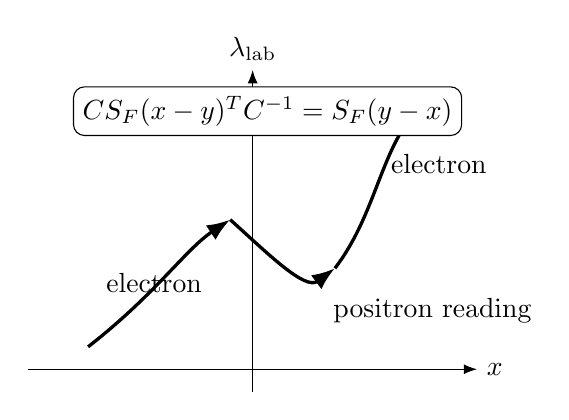
\begin{tikzpicture}[>=Latex,scale=0.95]
\draw[->] (-3,0)--(3,0) node[right] {$x$};
\draw[->] (0,-0.3)--(0,4.0) node[above] {$\lambda_{\rm lab}$};
\draw[very thick,->] (-2.2,0.3) .. controls (-1.3,1.0) and (-0.9,1.6) .. (-0.3,2.0);
\draw[very thick,->] (-0.3,2.0) .. controls (0.2,1.55) and (0.7,1.05) .. (1.1,1.35);
\draw[very thick,->] (1.1,1.35) .. controls (1.6,2.0) and (1.7,2.8) .. (2.25,3.55);
\node[anchor=east] at (-0.55,1.15) {electron};
\node[anchor=west] at (0.95,0.78) {positron reading};
\node[anchor=west] at (1.72,2.75) {electron};
\node[draw,rounded corners,fill=white] at (0.2,3.45) {$C S_F(x-y)^T C^{-1}=S_F(y-x)$};
\end{tikzpicture}
\caption{Feynman's switchback language can be stated without treating Wigner $T$ as a laboratory operation. The oppositely directed middle segment is the same Dirac line read with reversed momentum flow and conjugate charge assignment.}
\label{fig:switchback}
\end{figure}

\section{The interacting QED test}
For this subsection set $\hbar=c=1$. The free switchback identity is not enough. The simplest interacting theory must also respect the distinction between a half flip and a diagonal flip. Write
\begin{equation}\label{eq:qedlag}
 \mathcal L_{\rm QED}=-\frac14F_{\mu\nu}F^{\mu\nu}
 +\bar\psi(i\gamma^\mu D_\mu-m)\psi,
 \qquad D_\mu=\partial_\mu+ieA_\mu.
\end{equation}
Define $\psi^C=C\bar\psi^{\,T}$, with $C(\gamma^\mu)^TC^{-1}=-\gamma^\mu$. The Dirac current is odd under charge conjugation,
\begin{equation}
 \bar\psi^C\gamma^\mu\psi^C=-\bar\psi\gamma^\mu\psi,
\end{equation}
while the Maxwell kinetic term is unchanged by $A_\mu\mapsto-A_\mu$. Hence
\begin{equation}
 (\psi,A_\mu)\mapsto(\psi^C,-A_\mu)
\end{equation}
leaves Eq.~\eqref{eq:qedlag} invariant.

\begin{theorem}[QED conjugation dictionary]\label{thm:qedC}
For QED in flat spacetime, charge conjugation sends
\begin{equation}
 j^\mu\mapsto-j^\mu,\qquad A_\mu\mapsto-A_\mu,\qquad F_{\mu\nu}\mapsto-F_{\mu\nu},
\end{equation}
and leaves the action invariant. Equivalently, an electron line in a prescribed electromagnetic background is mapped to a positron line in the conjugate background. This is a symmetry relation between conjugate experiments, not an assertion that charge sign is individually unobservable in one fixed experiment.
\end{theorem}

The worldline interaction makes the diagonal structure even more transparent:
\begin{equation}\label{eq:worldint}
 S_{\rm int}[q,\gamma;A]=Q_\star q\int_\gamma A.
\end{equation}
Since $\int_{\gamma^{-1}}A=-\int_\gamma A$,
\begin{equation}\label{eq:worlddiag}
 S_{\rm int}[q,\gamma^{-1};A]=S_{\rm int}[-q,\gamma;A],
 \qquad
 S_{\rm int}[-q,\gamma^{-1};A]=S_{\rm int}[q,\gamma;A].
\end{equation}
The second identity is the classical diagonal quotient in its shortest form.

There is an important asymmetry of interpretation. In a laboratory the apparatus is held fixed, so replacing an electron by a positron is a \emph{relative} change and is observable. The diagonal transformation instead changes the line orientation and representation together. The orientation hypothesis asks whether this latter operation remains invisible after every dynamical and operational standard, not merely the Wilson phase, is transformed consistently.

\subsection{The CAR bridge and why pair production is neutral}
The orientation bookkeeping can be matched to the smallest charged fermionic Fock space without assigning negative physical energy to the opposite frequency orientation. Let $a^\dagger$ create the reference particle mode and $b^\dagger$ create its antiparticle mode. Define the dimensionless relative charge grading, the physical electric-charge operator and the positive Hamiltonian by
\begin{equation}\label{eq:CARQH}
 Q=N_a-N_b,\qquad
 \widehat Q_{\rm em}=Q_\star Q,\qquad
 H=\varepsilon(N_a+N_b),\qquad \varepsilon>0.
\end{equation}
For the electron convention $Q_\star=-e$, the $Q=+1$ state has electric charge $-e$ and the $Q=-1$ state has charge $+e$. Thus the one-particle states have opposite physical charge but the same positive energy. The diagonal-even orientation state
\begin{equation}
 (\alpha,\beta,\beta,\alpha)
\end{equation}
is intertwined with the one-particle Fock state
\begin{equation}\label{eq:orientationCARbridge}
 \mathcal B(\alpha,\beta,\beta,\alpha)=\alpha\,|e^-\rangle+\beta\,|e^+\rangle,
\end{equation}
and the orientation grading $\chi$ is carried to the Fock charge sign. Either orientation half flip exchanges the two coefficients; the positive Hamiltonian does not change sign.

\begin{theorem}[Neutral pair-creation selection rule]\label{thm:paircreation}
On the two-mode CAR algebra of Eq.~\eqref{eq:CARQH},
\begin{equation}
 [Q,a^\dagger]=a^\dagger,\qquad
 [Q,b^\dagger]=-b^\dagger,
\end{equation}
while the pair creator $P^\dagger=a^\dagger b^\dagger$ obeys
\begin{equation}\label{eq:paircommutators}
 \boxed{[Q,P^\dagger]=0,\qquad [H,P^\dagger]=2\varepsilon P^\dagger.}
\end{equation}
Thus an isolated charged half flip is not a charge-neutral process, whereas particle--antiparticle pair creation is.
\end{theorem}
\begin{proof}
Use $[Q,AB]=[Q,A]B+A[Q,B]$ and the two one-particle charge commutators. The charge terms cancel for $a^\dagger b^\dagger$. The Hamiltonian counts both created excitations and therefore contributes $\varepsilon+\varepsilon=2\varepsilon$.
\end{proof}

This theorem removes a misleading intuition: antimatter is not intrinsically heavier or endowed with negative physical energy. The obstruction to turning one charged excitation into its antiparticle at fixed laboratory standards is the conserved gauge charge. A neutral interaction can create both members together once the kinematic threshold and interaction dynamics are satisfied.

A complementary gauge test comes from a Majorana-type bilinear. If $\psi$ has $U(1)$ charge $Q_\psi$, then $\psi^T C\psi$ carries charge $2Q_\psi$. Hence a bare local particle--antiparticle mixing term is gauge neutral only for $Q_\psi=0$, or when an additional field supplies charge $-2Q_\psi$. This is why the orientation half-flip may be directly dynamical in a neutral sector while a charged sector requires compensation.

\section{Orientation exchanges self-dual and anti-self-dual fields}
Let $(M,g,\mathfrak o)$ be an oriented four-manifold. The Hodge operator depends on the orientation. Reversing $\mathfrak o$ changes the volume form by a sign and hence
\begin{equation}\label{eq:hodge}
 *_{-\mathfrak o}=-*_{\mathfrak o}.
\end{equation}
In Lorentzian signature, $*^2=-1$ on real two-forms. The self-dual decomposition is therefore made after complexification:
\begin{equation}\label{eq:lorhodge}
 *_{\mathfrak o}F_+=+iF_+,
 \qquad
 *_{\mathfrak o}F_-=-iF_-.
\end{equation}
Using Eq.~\eqref{eq:hodge}, the same $F_+$ obeys
\begin{equation}
 *_{-\mathfrak o}F_+=-iF_+,
\end{equation}
and similarly $F_-$ acquires the opposite label. Thus orientation reversal exchanges the $+i$ and $-i$ eigenspaces,
\begin{equation}
 \Lambda^2_{+,\mathbb C}(\mathfrak o)
 =\Lambda^2_{-,\mathbb C}(-\mathfrak o),
\end{equation}
with the Euclidean $\pm1$ statement recovered only in Euclidean signature. This exchange is exact and requires no cosmological second half.

In complexified Lorentzian representation theory,
\begin{equation}
 \mathfrak{so}(1,3)_\mathbb C\simeq
 \mathfrak{sl}(2,\mathbb C)_L\oplus\mathfrak{sl}(2,\mathbb C)_R,
\end{equation}
and an orientation-reversing Lorentz transformation such as parity exchanges the two chiral factors. Wigner time reversal is antiunitary and must be treated separately; it should not be identified with this geometric statement. The chirality operator itself contains the oriented volume element,
\begin{equation}
 \gamma^5=i\gamma^0\gamma^1\gamma^2\gamma^3,
\end{equation}
so its sign is orientation-sensitive. These facts make SD/ASD and L/R genuine candidates for representations of an orientation involution. They do not by themselves prove that electric charge, chirality and worldline orientation are one fundamental $\mathbb Z_2$.


\section{Chirality is orientation-sensitive}
The relation between spacetime orientation and chirality can be made exact. Let $e^a{}_{\mu}$ be an oriented tetrad and define
\begin{equation}
 \gamma^5=\frac{i}{4!}\,\epsilon_{abcd}\gamma^a\gamma^b\gamma^c\gamma^d,
 \qquad P_{L,R}=\frac{1\mp\gamma^5}{2}.
\end{equation}
Reversing the tetrad orientation changes the sign of the volume form. Holding the Clifford generators fixed as an unoriented algebra therefore sends
\begin{equation}\label{eq:g5flip}
 \epsilon_{abcd}\mapsto-\epsilon_{abcd},\qquad
 \gamma^5\mapsto-\gamma^5,
 \qquad P_L\leftrightarrow P_R.
\end{equation}

\begin{theorem}[Orientation--chirality exchange]\label{thm:chiralityorientation}
On an even-dimensional oriented Lorentzian spin manifold, reversal of the chosen orientation interchanges the two chiral spinor subbundles. In four dimensions this is Eq.~\eqref{eq:g5flip}.
\end{theorem}
\begin{proof}
The chirality operator is the Clifford action of the oriented volume element, up to the conventional phase required by the signature. Reversing orientation negates that volume element, hence negates $\gamma^5$. Its $\pm1$ eigenspaces are therefore exchanged.
\end{proof}

This result supplies an exact bridge that is stronger than a visual analogy: both Hodge duality and fermion chirality depend on the same choice of four-dimensional orientation. It still does not identify charge conjugation, Wigner $T$, or the spin-cover sign with orientation reversal. Those are additional structures.

\section{The common geometric pattern}
The previous sections establish several exact involutions but not their identity. It is useful to display what is known before proposing more.
\begin{equation}
\begin{array}{ccl}
\text{oriented gauge line} &:& (\gamma,R)\leftrightarrow(\gamma^{-1},R^*),\\[2mm]
\text{spin lift} &:& \psi\leftrightarrow-\psi\quad\text{over the same vector},\\[2mm]
\text{four-dimensional orientation} &:& \Lambda^2_+\leftrightarrow\Lambda^2_-,\\[2mm]
\text{Lorentz chirality under parity/orientation reversal} &:& (\tfrac12,0)\leftrightarrow(0,\tfrac12),\\[2mm]
\text{celestial shadow} &:& (\Delta,J)\leftrightarrow(2-\Delta,-J).
\end{array}
\end{equation}
The first three lines are geometric identifications of standard structures. The last two require the stated transformation and should not be silently identified with charge conjugation or Wigner $T$.

\begin{definition}[Orientation lift hypothesis]\label{def:lift}
A theory has a physical orientation lift if there exists a double cover
\begin{equation}
 \pi:\widetilde{\mathcal X}\to\mathcal X,
 \qquad \iota^2=1,\qquad \pi\circ\iota=\pi,
\end{equation}
such that every operational observable factors through $\pi$, while some intermediate variables used in the local description transform nontrivially under $\iota$.
\end{definition}

Definition~\ref{def:lift} is the strong proposal of the paper. The spinor/vector relation is an unquestioned example of this logic for a particular set of observables. The claim that charge/time orientation, chirality, duality sector and celestial orientation are all images of the same $\iota$ is a conjectural extension and must be demonstrated by commuting maps, not by counting binary labels.

\section{One sphere, two orientations}\label{sec:onesphere}
The celestial sphere is the Riemann sphere
\begin{equation}
 S^2\simeq\mathbb{CP}^1\simeq\mathbb C\cup\{\infty\}.
\end{equation}
The same underlying sphere admits two opposite orientations. Several maps must be distinguished:
\begin{equation}
 z\mapsto \bar z \quad\text{(orientation reversal)},\qquad
 z\mapsto\frac1z \quad\text{(holomorphic inversion)},
\end{equation}
while
\begin{equation}
 z\mapsto\frac1{\bar z}
\end{equation}
combines them, exchanges the interior and exterior of the unit circle, and fixes $|z|=1$.

Likewise radial inversion becomes time-like reflection after logarithmic parametrization:
\begin{equation}
 r=e^u,\qquad r\mapsto r^{-1}\quad\Longleftrightarrow\quad u\mapsto-u.
\end{equation}
This is the mathematically clean bridge between scale inversion and an orientation variable. It is not a proof that radial time is physical proper time.

For celestial weights $\Delta=h+\bar h$ and $J=h-\bar h$, the standard shadow map sends
\begin{equation}
 (h,\bar h)\mapsto(1-h,1-\bar h),
 \qquad
 (\Delta,J)\mapsto(2-\Delta,-J).
\end{equation}
Complex conjugation and shadow are distinct operations. The anti-linear composition
\begin{equation}\label{eq:antilinear}
 \mathcal R:\Delta\mapsto2-\bar\Delta
\end{equation}
has fixed locus
\begin{equation}
 \Delta=2-\bar\Delta\quad\Longleftrightarrow\quad\Re\Delta=1,
\end{equation}
which is the celestial principal-series axis. Under the bookkeeping normalization $\Delta=2s$, Eq.~\eqref{eq:antilinear} becomes $s\mapsto1-\bar s$ with fixed locus $\Re s=1/2$. This is a fixed-locus identity, not a proof of the Riemann hypothesis.

\begin{proposition}[Anti-linear fixed locus]\label{prop:fixed}
Let $\mathcal R(\Delta)=2-\bar\Delta$. Then $\mathcal R^2=1$ and
\begin{equation}
 \operatorname{Fix}(\mathcal R)=\{\Delta\in\mathbb C:\Re\Delta=1\}.
\end{equation}
On the principal series $\Delta=1+i\lambda$, bare shadow and complex conjugation each send $\lambda\mapsto-\lambda$, whereas their composition fixes $\Delta$ pointwise.
\end{proposition}
\begin{proof}
$\mathcal R^2(\Delta)=2-\overline{2-\bar\Delta}=\Delta$. The fixed-point equation $\Delta=2-\bar\Delta$ is equivalent to $\Delta+\bar\Delta=2$, hence $\Re\Delta=1$. Substitution of $\Delta=1+i\lambda$ gives the final statement.
\end{proof}

\subsection{The finite real structure and the critical-line reflection}\label{subsec:finitecriticalreal}
The four-lift correction above gives a precise finite analogue of the anti-holomorphic fixed-locus map, but it is important to state the analogy at the correct level. Center the arithmetic coordinate by
\begin{equation}
 \nu=s-\frac12.
\end{equation}
Then the two elementary operations are
\begin{equation}\label{eq:centeredRHops}
 \rho(\nu)=-\bar\nu,
 \qquad
 \sigma(\nu)=-\nu.
\end{equation}
The first is anti-holomorphic and involutive, with
\begin{equation}
 \operatorname{Fix}(\rho)=i\mathbb R,
\end{equation}
which is exactly $\Re s=1/2$. The second is the centered shadow reflection; restricted to $\nu=i\lambda$ it sends $\lambda\mapsto-\lambda$.

On the finite carrier, $\mathsf D$ obeys
\begin{equation}
 \mathsf D^2=1,
 \qquad
 \mathsf D I_q=-I_q\mathsf D,
\end{equation}
so it is anti-linear for the microscopic complex structure $I_q$, and its fixed locus is the real form $\mathcal H_{\mathsf D}$. The temporal half flip $R_t$ commutes with $\mathsf D$, preserves $\mathcal H_{\mathsf D}$, and reverses the surviving grading $\chi$. Thus the two pairs have the same algebraic architecture:
\begin{center}
\begin{tabular}{>{\raggedright\arraybackslash}p{0.30\textwidth} >{\raggedright\arraybackslash}p{0.54\textwidth}}
\toprule
finite orientation carrier & centered $s$-plane\\
\midrule
$\mathsf D$: $I_q$-anti-linear involution; fixed real form & $\rho(\nu)=-\bar\nu$: anti-holomorphic involution; fixed critical line\\
$R_t$: linear half flip on the fixed form; $\chi\mapsto-\chi$ & $\sigma(\nu)=-\nu$: linear shadow reflection on the critical line; $\lambda\mapsto-\lambda$\\
\bottomrule
\end{tabular}
\end{center}
This table is an exact comparison of two involution architectures, not an identification of their physical carriers and not a proof of RH. The cross-theory dictionary remains a theorem target. The finite and centered fixed-locus statements are encoded in \path{OrientationCriticalRealStructureBridge.lean}; release-level kernel verification is tracked in the companion repository.


\subsection{The principal-series Hilbert lift}

The fixed-locus statement becomes more informative when the celestial transform is normalized by the one-particle Hilbert measure. For
\begin{equation}
 q^\mu(z,\bar z)=(1+|z|^2,z+\bar z,-i(z-\bar z),1-|z|^2),
 \qquad p^\mu=\omega q^\mu,
\end{equation}
a direct Jacobian calculation gives
\begin{equation}\label{eq:masslessmeasure}
 \frac{d^3p}{2p^0}=2\omega\,d\omega\,d^2z.
\end{equation}
Thus, if $u=\log\omega$ and
\begin{equation}
 g(u,z)=\sqrt2\,e^u f(e^u,z),
\end{equation}
then
\begin{equation}
 \|f\|^2=\int du\,d^2z\,|g(u,z)|^2.
\end{equation}
Ordinary Fourier--Plancherel transformation in $u$ therefore gives
\begin{equation}
 F(\lambda,z)=\frac{1}{\sqrt\pi}\int_0^\infty
 d\omega\,\omega^{i\lambda}f(\omega,z),
\end{equation}
so comparison with the celestial Mellin kernel $\omega^{\Delta-1}$ yields
\begin{equation}\label{eq:principalplancherel}
 \boxed{\Delta=1+i\lambda,\qquad \lambda\in\mathbb R.}
\end{equation}
This is the unitary principal-series line in the massless one-particle basis; it is not a dynamical equation for $\Delta$~\cite{PasterskiShao2017,Pasterski2021}.

The normalized celestial shadow operator
\begin{equation}
 \mathsf S_{\Delta,J}:\mathcal H_{\Delta,J}\longrightarrow
 \mathcal H_{2-\Delta,-J}
\end{equation}
may be chosen so that
\begin{equation}\label{eq:shadowsquare}
 \mathsf S_{2-\Delta,-J}\mathsf S_{\Delta,J}
 =(-1)^{2J}I
\end{equation}
for integer or half-integer $J$~\cite{Pasterski2021}. Let
\begin{equation}
 \mathcal C_{\Delta,J}:\mathcal H_{\Delta,J}\longrightarrow
 \mathcal H_{\bar\Delta,-J}
\end{equation}
denote coefficient conjugation in the celestial realization. On the principal series $\bar\Delta=2-\Delta$, so shadow and conjugation have the same target representation but remain different operators: $\mathsf S$ is linear and nonlocal on the sphere, whereas $\mathcal C$ is anti-linear.

\begin{proposition}[Real/quaternionic principal-series lift]\label{prop:celestialquat}
On the principal series define the anti-linear endomorphism
\begin{equation}
 \widehat{\mathcal R}_{\Delta,J}
 :=\mathsf S_{2-\Delta,-J}\mathcal C_{\Delta,J}.
\end{equation}
With the normalization of Eq.~\eqref{eq:shadowsquare},
\begin{equation}
 \boxed{\widehat{\mathcal R}_{\Delta,J}^{\,2}=(-1)^{2J}I.}
\end{equation}
Hence integer-spin fibres carry a real structure, while half-integer-spin fibres carry a quaternionic structure with $\widehat{\mathcal R}^{\,4}=I$.
\end{proposition}

\begin{proof}
Complex conjugation of the shadow kernel interchanges the two conjugate principal-series kernels, so
\begin{equation}
 \mathcal C_{\Delta,J}\mathsf S_{2-\Delta,-J}
 =\mathsf S_{\Delta,J}\mathcal C_{2-\Delta,-J}.
\end{equation}
Since $\mathcal C_{2-\Delta,-J}\mathcal C_{\Delta,J}=I$, the square reduces to Eq.~\eqref{eq:shadowsquare}.
\end{proof}

The label map $\Delta\mapsto2-\bar\Delta$ still squares to the identity for every $J$. Proposition~\ref{prop:celestialquat} says that its natural Hilbert-space lift can retain the central spin sign. This is exactly the distinction between an order-two projective action and an order-four spinorial lift. It also prevents another conflation: a wedge modular conjugation is an antiunitary geometric operator, while the celestial shadow is a linear Knapp--Stein-type integral transform. Equality of their representation labels on $\Re\Delta=1$ does not make the operators equal; modular localization supplies a separate real-subspace construction~\cite{BGL2002}.

\begin{figure}[t]
\centering
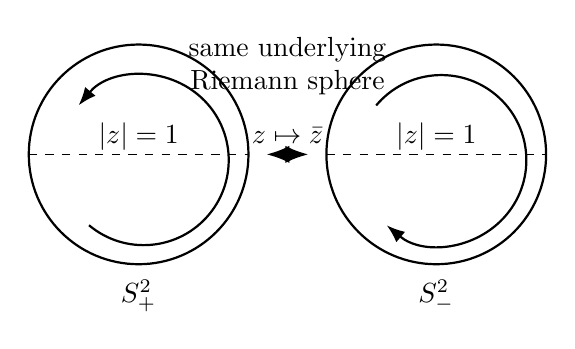
\begin{tikzpicture}[>=Latex,scale=0.9]
\draw[thick] (0,0) circle (1.55);
\draw[thick] (4.2,0) circle (1.55);
\draw[->,thick] (-0.7,-1.0) arc[start angle=230,end angle=500,radius=1.2];
\draw[<-,thick] (3.5,-1.0) arc[start angle=230,end angle=500,radius=1.2];
\node at (0,-2.0) {$S^2_{+}$};
\node at (4.2,-2.0) {$S^2_{-}$};
\draw[<->,very thick] (1.8,0)--(2.4,0) node[midway,above] {$z\mapsto\bar z$};
\node[align=center] at (2.1,1.25) {same underlying\\Riemann sphere};
\draw[dashed] (-1.55,0)--(1.55,0);
\draw[dashed] (2.65,0)--(5.75,0);
\node at (0,0.25) {$|z|=1$};
\node at (4.2,0.25) {$|z|=1$};
\end{tikzpicture}
\caption{Opposite complex orientations do not require two different celestial spheres. They are two orientations of the same underlying $S^2$. Holomorphic inversion, complex conjugation and $z\mapsto1/\bar z$ remain distinct maps.}
\label{fig:sphere}
\end{figure}

\begin{figure}[t]
\centering
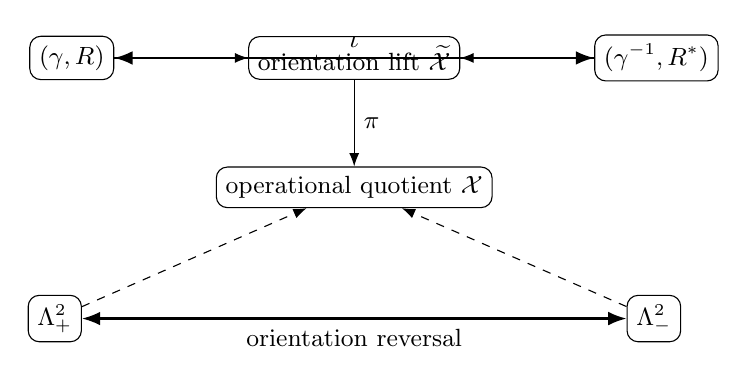
\begin{tikzpicture}[node distance=11mm and 17mm,>=Latex, every node/.style={font=\small}]
\node (or) [draw,rounded corners] {orientation lift $\widetilde{\mathcal X}$};
\node (obs) [draw,rounded corners,below=of or] {operational quotient $\mathcal X$};
\node (g) [draw,rounded corners,left=of or] {$(\gamma,R)$};
\node (gd) [draw,rounded corners,right=of or] {$(\gamma^{-1},R^*)$};
\node (sd) [draw,rounded corners,below left=of obs] {$\Lambda^2_+$};
\node (asd) [draw,rounded corners,below right=of obs] {$\Lambda^2_-$};
\draw[<->,thick] (g)--node[above]{$\iota$}(gd);
\draw[->] (or)--node[right]{$\pi$}(obs);
\draw[<->,thick] (sd)--node[below]{orientation reversal}(asd);
\draw[dashed,->] (g)--(or);\draw[dashed,->] (gd)--(or);
\draw[dashed,->] (sd)--(obs);\draw[dashed,->] (asd)--(obs);
\end{tikzpicture}
\caption{The proposed architecture. Solid arrows are exact structures; dashed arrows indicate the still-unproved identification that would make them representations of one physical orientation lift.}
\label{fig:master}
\end{figure}

\section{The googly question, stated without cheating}
The nonlinear twistor correspondence naturally privileges one duality sector. The googly problem asks for the opposite interacting sector without simply adjoining an unrelated copy. Equation~\eqref{eq:hodge} shows that orientation reversal exchanges SD and ASD geometry, and the celestial shadow reverses helicity. These are necessary ingredients for an orientation-based answer, but they are not sufficient.

\begin{conjecture}[Orientation reconstruction criterion]\label{conj:googly}
A genuine orientation resolution of the googly problem requires a canonical map from nonlinear twistor data in one oriented sector to nonlinear data in the opposite sector such that: (i) the reconstructed fields satisfy the full nonlinear field equations; (ii) the map reproduces the appropriate MHV/anti-MHV amplitudes including phases and normalizations; and (iii) applying the orientation map twice returns the original physical data modulo the relevant gauge equivalence.
\end{conjecture}

This criterion deliberately retracts the stronger earlier claim that bare shadow symmetry alone solves the googly problem. Recent work~\cite{Adamo2026} has constructed a non-self-dual Schwarzschild geometry from holomorphic data in a self-dual Taub--NUT twistor space, showing both that the problem remains active and that nontrivial reconstruction can occur in special cases. A universal theorem must meet Conjecture~\ref{conj:googly}, not merely exchange helicity labels.

There is, however, a sharper geometric route than the earlier slogan suggests. The ordinary Penrose correspondence is not a pointwise map from spacetime to twistor space. Its linear-algebra core is the flag correspondence
\begin{equation}
 \mathbb{PT}=\mathbb P(V)\ \longleftarrow\ F_{1,2}(V)\ \longrightarrow\ \Gr(2,V),\qquad V\simeq\mathbb C^4,
\end{equation}
where $F_{1,2}(V)=\{\ell\subset W\subset V:\dim\ell=1,\dim W=2\}$. The Penrose transform is a pull--push transform through this incidence space~\cite{WardWells}. For a subspace $W\subset V$, let $W^0\subset V^*$ denote its annihilator. Inclusion reverses exactly,
\begin{equation}\label{eq:annihilatorreverse}
 \ell\subset W\quad\Longrightarrow\quad W^0\subset\ell^0.
\end{equation}
Thus annihilator duality sends a $(1,2)$ twistor flag to a $(2,3)$ flag in the dual vector space. In four dimensions this statement is sharper than it first appears. If $\dim \ell=1$ and $\dim W=2$, then
\begin{equation}\label{eq:annihilatordims}
 \dim W^0=2,\qquad \dim \ell^0=3.
\end{equation}
Consequently annihilation gives a canonical point map on the spacetime Grassmannian, $\Gr(2,V)\to\Gr(2,V^*)$, but it does \emph{not} give a pointwise map $\mathbb{PT}=\mathbb P(V)\to\mathbb{PT}^*=\mathbb P(V^*)$: the annihilator of a twistor line is a hyperplane, not a dual-twistor line. The annihilator/coannihilator round trip nevertheless recovers the complete flag exactly. Thus the natural googly object is a reversible \emph{correspondence}, and any field-level map must be an induced Radon/Fourier/Penrose intertwiner rather than a naive replacement of one projective twistor by another.

There is also an exact homogeneity check. Write $n=2h\in\mathbb Z$ for doubled helicity. The ordinary Penrose transform represents helicity $h$ by twistor data of homogeneity
\begin{equation}\label{eq:twistorweight}
 k=2h-2=n-2,
\end{equation}
whereas the corresponding dual-twistor representation has homogeneity $-2h-2=-n-2$~\cite{WardWells,ArkaniHamed2010}. A Fourier transform in four twistor variables changes homogeneous degree by
\begin{equation}\label{eq:fourierweight}
 k\longmapsto -k-4.
\end{equation}
Therefore
\begin{equation}\label{eq:weightflip}
 -(n-2)-4=-n-2=2(-h)-2.
\end{equation}
The four-dimensional Fourier shift is thus exactly the homogeneity required for helicity reversal once dual twistor space is identified with the opposite-oriented twistor description. The map $k\mapsto-k-4$ is an involution with unique fixed weight $k=-2$, the scalar case; photons pair $0\leftrightarrow-4$ and gravitons $2\leftrightarrow-6$. This does not yet prove the cohomological transform exists on every class or that it extends nonlinearly, but it removes the homogeneity mismatch as a possible obstruction.

There is a useful precedent for treating the Penrose transform itself as a square-root operation rather than merely a dictionary between two sets of variables. In linearized higher-spin theory on $AdS_4$, Neiman showed that a twistor delta-function implements a spacetime CPT reflection by conjugation in the higher-spin star algebra, while one-sided multiplication by the same kernel gives the Penrose transform; in that precise model the Penrose transform is therefore a ``square root of CPT''~\cite{Neiman2017}. This result does \emph{not} solve the googly problem for Yang--Mills or Einstein gravity, and the higher-spin star algebra should not be imported into those theories by analogy.

The finite-dimensional square-root question can now be answered more precisely in the present geometry. Section~\ref{sec:grassmass} constructs a global Klein-quadric map $\mathsf T_K$ whose odd Pin lift exchanges twistor and dual-twistor half-spin modules and whose square covers total conformal inversion. A compatible Fourier kernel then gives an order-four integral operator $\mathcal G_T$ with
\begin{equation}\label{eq:googlysqrt}
 \boxed{\mathcal G_T^{\,2}=\Gamma^*,\qquad \mathcal G_T^{\,4}=I,}
\end{equation}
on the linear carrier, with the central spin sign restored on homogeneous representatives. Thus Eq.~\eqref{eq:googlysqrt} is no longer merely an abstract algebraic target at the finite linear level. What remains open is the physically harder statement: descent to the appropriate Penrose cohomology/distribution spaces with the required reality conditions, followed by a \emph{nonlinear} reconstruction of generic Yang--Mills or Einstein data. In particular, $\Gamma$ is total conformal spacetime inversion, not by itself reversal of the four-orientation. The latter still acts through $*_{\mathfrak o}\mapsto-*_{\mathfrak o}$ and must be combined with the twistor/dual-twistor incidence map when testing SD$\leftrightarrow$ASD dynamics.

A second correction is equally important. Applying the Hodge star to a two-form does not by itself exchange the SD and ASD eigenspaces. In Euclidean signature $*^2=1$, so $*$ acts as $+1$ on $\Lambda^2_+$ and $-1$ on $\Lambda^2_-$. What exchanges the sector labels is reversal of the four-orientation, which changes the operator itself, $*_{-\mathfrak o}=-*_{\mathfrak o}$. The same underlying two-form that was self-dual for $\mathfrak o$ is therefore anti-self-dual for $-\mathfrak o$. The Lorentzian complexified statement is identical with the eigenvalues $\pm i$. The googly construction must therefore combine incidence duality with orientation reversal; Hodge complement alone is not the SD$\leftrightarrow$ASD map.

\section{The electroweak obstruction and what it selects}
The strongest version of the orientation hypothesis meets its first serious obstacle in the Standard Model. The gauge group contains $SU(2)_L$, not a parity-symmetric pair $SU(2)_L\times SU(2)_R$ with equal low-energy couplings. Parity is therefore not a symmetry of the observed weak interactions, and measured CP violation prevents replacing this fact by a naive statement that ``left'' and ``right'' are merely names.

This does not immediately kill a \emph{global} orientation quotient, because a complete conjugation would also conjugate the representations, couplings, states and observer standards. But it changes the burden of proof. A viable formulation must exhibit an isomorphism between the full Standard Model on an oriented spacetime $(M,\mathfrak o)$ and the conjugate theory on $(M,-\mathfrak o)$, including Yukawa matrices and the CKM/PMNS phases, such that all dimensionless probabilities available to an internal observer agree after the dictionary is applied.

\begin{conjecture}[Electroweak orientation test]\label{conj:EW}
There exists a complete orientation-conjugation functor $\mathfrak C$ acting simultaneously on spacetime orientation, Lorentz chirality, gauge representations and complex couplings such that every gauge-invariant Standard-Model probability satisfies
\begin{equation}
 \mathcal P_{\mathfrak o}[\mathcal E]
 =\mathcal P_{-\mathfrak o}[\mathfrak C(\mathcal E)].
\end{equation}
If no such functor exists once the physical CP-violating invariants are included, the strong orientation hypothesis is false.
\end{conjecture}

The point is deliberately sharper than saying that CPT is a symmetry. CPT already guarantees equality of appropriately conjugated processes under the assumptions of local relativistic QFT. The additional claim under test is that the labels ``matter'', ``left'' and ``forward'' have no observer-independent sign beyond that complete relational correspondence.

A useful invariant stress test is the Jarlskog combination
\begin{equation}
 J=\operatorname{Im}(V_{ij}V_{kl}V^*_{il}V^*_{kj}),
\end{equation}
which changes sign under complex conjugation of the CKM matrix. A mere relabeling that leaves the experimental orientation standards fixed cannot erase the sign of a CP-odd asymmetry. A successful complete orientation dictionary must instead map the process, its conjugate, and the pseudoscalar orientation used to define the asymmetry together. This is exactly the sort of observable that can distinguish a genuine quotient from a verbal one.


\subsection{The CP-odd invariant does not disappear}
For three quark generations a rephasing-invariant measure of CP violation is~\cite{Jarlskog1985,PDGCP2024}
\begin{equation}\label{eq:J}
 J=\Im\!\left(V_{ij}V_{kl}V^*_{il}V^*_{kj}\right)
\end{equation}
for any choice of distinct rows and columns with the usual correlated sign. Complex conjugation of the CKM matrix gives
\begin{equation}\label{eq:Jflip}
 V\mapsto V^*\quad\Longrightarrow\quad J\mapsto-J.
\end{equation}
The sign flip is physical at fixed laboratory conventions: CP-conjugate decay asymmetries reverse. A proposed \emph{complete} orientation quotient cannot erase this fact. It must instead map the experiment, the flavour convention, the prepared state and the sign convention for the asymmetry to their conjugates so that the same dimensionless relational statement is recovered by the conjugate observer.

\begin{test}[Jarlskog test]\label{test:J}
Let $\iota_{\rm SM}$ be a candidate complete orientation involution on Standard-Model data. It must induce $V\mapsto V^*$ and hence $J\mapsto-J$ on the couplings while simultaneously mapping every CP-odd operational observable $A$ to its conjugate convention $A'=-A$. If there exists a convention-independent scalar observable whose numerical value is odd under $\iota_{\rm SM}$ after the entire apparatus dictionary is applied, the strong orientation quotient is false.
\end{test}

The distinction is important. Measured CP violation is not evidence against CPT, and it cannot be removed by relabelling a single subsystem. The orientation proposal survives only if the \emph{whole} conjugate experiment is isomorphic to the original experiment, exactly as demanded by Principle~\ref{prin:op}.

There is also a stronger bundle-level test than CP covariance alone. A universal local diagonal spin--gauge quotient requires a gauge factor whose central order-two element has the required spin--charge action on every fermion. The minimal Standard Model does not supply such a universal $U(1)$ spin--charge structure. Section~\ref{subsec:BLcompletion} shows that this obstruction is highly selective rather than fatal: with one right-handed neutrino per generation, $X=3(B-L)$ gives odd charge to every fermion, even charge to the Higgs, and cancels all local and mixed gravitational anomalies.

\section{Observers, records, and the inaccessible opposite arrow}
The microscopic sign $t$ and the thermodynamic arrow live on the same timelike geometry but are not the same variable. A Lorentzian metric supplies two orientations of each timelike line. An observer chooses one by a future-directed unit tangent $u^\mu$; a microscopic phase then has the relative sign $t_u(k)$ of Eq.~\eqref{eq:tphasecovariant}. No second time dimension is required.

A macroscopic observer is different from an elementary phase because it is a record-bearing many-body system. For an event $x$, present records can contain correlations whose causes lie in $J^-(x)$. This motivates the operational definition
\begin{equation}\label{eq:recordfuture}
 \mathfrak t_{\rm rec}=\hbox{the orientation along which new stable records can be accumulated}.
\end{equation}
For ordinary macroscopic matter the thermodynamic arrow is aligned with this record orientation,
\begin{equation}\label{eq:entropyrecord}
 \frac{dS_{\rm coarse}}{d\tau_{\rm rec}}\ge0
\end{equation}
statistically. Equation~\eqref{eq:entropyrecord} is a statement about a coarse-grained history, not about an intrinsic entropy carried by a single electron.

\begin{theorem}[Mass--observation theorem]\label{thm:massobservation}
Let a localized physical observer be a record-bearing system whose perspective is represented by a nonconstant family of internal record states $R(\tau)$ ordered by the invariant proper time $\tau$ along a centre worldline $\gamma$. Wherever distinct records are formed, $d\tau>0$ and $\gamma$ is timelike. If the system admits a total four-momentum of the usual massive form
\begin{equation}
 P^\mu=M U^\mu,\qquad U^\mu=\frac{d\gamma^\mu}{d\tau},
\end{equation}
then
\begin{equation}
 \boxed{M>0.}
\end{equation}
A null worldline, for which $d\tau=0$, cannot by itself carry a nontrivial proper-time-ordered observer history.
\end{theorem}
\begin{proof}
By definition, two distinct record states require a nonzero invariant interval of the ordering parameter. Since that parameter is proper time, $d\tau>0$ implies $ds^2=-c^2d\tau^2<0$ in the mostly-plus convention, so the centre curve is timelike and a normalized four-velocity $U$ exists. The total momentum then satisfies $P^2=-M^2c^2<0$, which excludes $M=0$. Conversely a null trajectory has $d\tau=0$ and therefore supplies no nontrivial proper-time parameter on which such an observer history can be indexed.
\end{proof}
The theorem is a necessity statement, not a sufficiency statement. It does not say that every massive system is an observer, and it does not forbid massless fields from carrying information inside a massive record-forming apparatus.

\begin{proposition}[Record obstruction to an operational arrow flip]\label{prop:recordobstruction}
Let $R(x)$ denote the complete physical record state of an observer at $x$, and suppose $R(x)$ contains correlations with events in the observer's causal past but no controllable information supplied from its causal future. A transformation that reverses only the observer's declared time orientation while leaving $R(x)$ fixed is operationally incomplete: the retained records still select the original causal orientation. A complete reversal must transform the record state and the standards by which those correlations are interpreted as well.
\end{proposition}
\begin{proof}
The physical correlations in $R(x)$ identify the set of events from which information has reached $x$. Relabelling the opposite cone ``past'' without transforming those correlations does not move their causal sources and therefore leaves an operational witness of the original orientation. Removing that witness requires transforming $R(x)$ together with the causal and measurement dictionary. The transformed observer then has no retained record from which to compare the two orientations.
\end{proof}

The same statement can be written directly in the $q,t$ language. If the observer's time orientation is reversed while the charge standard is held fixed, every observer-relative microscopic temporal sign changes,
\begin{equation}\label{eq:observerreverseqt}
 u^\mu\mapsto-u^\mu
 \quad\Longrightarrow\quad
 t_u(k)\mapsto-t_u(k),\qquad \chi=qt\mapsto-\chi.
\end{equation}
Thus matter would be assigned the antimatter sign relative to the unreversed charge standard. If the charge standard is reversed as well,
\begin{equation}\label{eq:completeanti}
 (q,t)\longmapsto(-q,-t),\qquad \chi\longmapsto\chi,
\end{equation}
the relational particle class is unchanged. This is the precise content of the statement that neither complete sign assignment is absolute: the $++$ observer may call itself ordinary and the $--$ observer may do the same, because each has transformed the standards used to make the comparison.

\begin{conjecture}[Mass-clock inheritance]\label{conj:massclock}
For massive matter, the record arrow used by macroscopic record-forming observers is inherited, after decoherence and coarse graining, from a collective ordering of the constituent proper-time phases
\begin{equation}
 d\varphi=-\frac{mc^2}{\hbar}\,d\tau_{\rm or}.
\end{equation}
The thermodynamic record arrow is an emergent order parameter on this common timelike geometry, not a second time coordinate and not a majority vote of independent microscopic $t$ signs.
\end{conjecture}
This must ultimately be derived from an open-system model of many relativistic degrees of freedom. In particular, the theory must show how a stable record orientation emerges while the fundamental equations and the orientation cover retain their conjugate lift.

\begin{theorem}[Quotient of an invariant observable algebra]\label{thm:obsalg}
Let $\iota$ be an involution of a state space $\widetilde{\mathcal S}$ and suppose the operational algebra $\mathcal A_{\rm op}$ satisfies $O\circ\iota=O$ for every $O\in\mathcal A_{\rm op}$. Then no experiment whose statistics are functions only of elements of $\mathcal A_{\rm op}$ can distinguish $x$ from $\iota x$.
\end{theorem}
\begin{proof}
Every probability distribution constructed from the operational observables has identical arguments on $x$ and $\iota x$. Hence all such distributions coincide. Any distinguishing experiment would define an observable outside the assumed invariant algebra.
\end{proof}

\begin{conjecture}[Observer-orientation hypothesis]\label{conj:observer}
Fundamental dynamics admits conjugate orientation lifts with no observable absolute preference. Embedded record-forming observers operationally select one orientation through the joint organization of causal accessibility, thermodynamic records and their internal standards. Complete conjugation of system plus observer leaves relational observables invariant; incomplete conjugations are observable as opposite sectors.
\end{conjecture}

The hypothesis does not say that entropy causes causality, nor that an intact observer can watch its own records run backward. It says that ``past'' and ``future'' are the two orientations of one causal time structure, while an observer's records select one of them internally. The next section on thermodynamics makes the time-reflection statement precise.

\section{The black-mirror horizon as a branched orientation cover}\label{sec:blackmirror}
The black-mirror construction of Tzanavaris, Boyle and Turok~\cite{TzanavarisBoyleTurok2025} supplies a concrete spacetime geometry in which a two-sided exterior is represented by a folded radial coordinate rather than by an ordinary black-hole interior. In the static case their analytic radial variable may be written in geometric units as
\begin{equation}\label{eq:mirrorradius}
 r(\sigma)=2m\left[1+\left(\frac{\sigma}{4m}\right)^2\right]
 =2m+\frac{\sigma^2}{8m},\qquad m>0.
\end{equation}
The involution
\begin{equation}
 D_H:\sigma\mapsto-\sigma
\end{equation}
leaves the exterior radius exactly invariant,
\begin{equation}\label{eq:mirrorsheet}
 \boxed{r(-\sigma)=r(\sigma)}.
\end{equation}
Away from the horizon, the two lifts $\pm\sigma$ are distinct; at the horizon they coalesce because
\begin{equation}
 D_H\sigma=\sigma\quad\Longleftrightarrow\quad\sigma=0,
\end{equation}
and
\begin{equation}
 r(0)=2m.
\end{equation}
Thus the radial geometry is locally a folded/branched double cover of the ordinary exterior coordinate. The base coordinate depends only on $\sigma^2$, and the odd first-order response vanishes at the branch point.

\begin{proposition}[Horizon double-cover algebra]\label{prop:horizoncover}
For $r(\sigma)$ in Eq.~\eqref{eq:mirrorradius},
\begin{equation}
 r(\sigma)-2m=\frac{\sigma^2}{8m},\qquad
 \frac{r(\sigma)-r(0)}{\sigma}=\frac{\sigma}{8m}\quad(\sigma\neq0).
\end{equation}
Hence every observable depending only on $r$ is blind to the sheet sign, and the secant slope to the horizon tends to zero as $\sigma\to0$.
\end{proposition}
\begin{proof}
Both identities follow directly from Eq.~\eqref{eq:mirrorradius}. Evenness under $\sigma\mapsto-\sigma$ proves sheet blindness of any function of $r$ alone.
\end{proof}

\subsection{The fold is a Stueckelberg turnaround in the radial coordinate}\label{subsec:mirrorstueckelberg}
The coordinate $\sigma$ advances monotonically through the branch point while the observable radius folds: $dr/d\sigma=\sigma/4m$ changes sign at $\sigma=0$. That is the structure of Remark~\ref{rem:stueckelbergpriority} with the roles relabelled. In Stueckelberg's worldline mechanics an invariant parameter advances monotonically while the laboratory coordinate $x^0$ folds, and a pair process is one continuous line whose $\dot x^0$ changes sign. In Eq.~\eqref{eq:mirrorradius} the parameter is $\sigma$, the folded coordinate is $r$, and both fold laws are quadratic about the turning point. The black mirror is therefore the 1941 turnaround in the radial coordinate rather than the time coordinate, realized by a genuine coordinate on the doubled manifold and not by an external chronology.

\subsection{The same square-root cover at the other null locus}\label{subsec:mirrorsqrt}
Inverting Eq.~\eqref{eq:mirrorradius} gives
\begin{equation}\label{eq:mirrorsqrt}
 \sigma=\pm\sqrt{8m\,(r-2m)},
\end{equation}
a two-valued square root branched on $r=2m$. Section~\ref{subsec:sqrtmonodromy} found the determinant cover in the form $s=\pm\sqrt{\det A}=\pm\sqrt{x\cdot x}$, branched on $x\cdot x=0$ by Eq.~\eqref{eq:detisinterval}. Both are pullbacks of the universal square-root cover $z\mapsto z^2$, branched over a null hypersurface: the horizon in the first case, the light cone in the second. The black-mirror sheet and the determinant deck are therefore the same local cover evaluated over the two null loci of the geometry. As with the light-cone meridian and the Compton circuit in Section~\ref{subsec:sqrtmonodromy}, this identifies the cover type and not the physical loops.

\subsection{Which gluing, and what annihilates}\label{subsec:mirrorgluing}
Two gluings of the orientation carrier across the fold are mathematically possible, and they are not compatible.
\begin{enumerate}[leftmargin=2.2em]
\item \emph{Diagonal gluing.} The far sheet carries $(q,t)\mapsto(-q,-t)$, so $\chi$ is preserved and the object on the far sheet is the other lift of the same relational class.
\item \emph{Half-flip gluing.} The far sheet carries a single sign reversal, so $\chi\mapsto-\chi$ and the far sheet holds the conjugate class. The fold is then an annihilation vertex, neutral by Theorem~\ref{thm:paircreation}.
\end{enumerate}
A description in which the particle meets its CPT-related partner at the horizon is the second option, since a CPT partner has the opposite relational class. The present framework requires the first: the diagonal is the operation shown to be unobservable, and the half flip is the operation shown to change the particle class. The target is accordingly a spin--gauge lift over the doubled exterior in which the horizon gluing acts on the orientation carrier by the diagonal involution preserving $\chi$. The identification of $\sgn\sigma$ with the microscopic sign $t$ remains a new bundle-level hypothesis and is not proved here.

Under the diagonal gluing nothing annihilates. There is one worldline, which folds at the branch point, where the lift and its sheet image are the same event; both halves carry the same $\chi$. The appearance of a particle meeting an antiparticle at the horizon is a sheet-labelling artefact in exactly the sense that the appearance of a pair in Stueckelberg's diagram is a slicing artefact.

This also removes the need for any spacelike segment. Turning a future-directed timelike worldline into a past-directed one \emph{within spacetime} requires crossing the spacelike region, so the constraint $\dot x^2$ fixed must fail at the turning point; the off-shell development of Stueckelberg's programme relaxes the mass shell for exactly this reason. In the present construction the orientation reversal is not a rotation of the spacetime tangent vector. It is the transverse half turn $\zeta_\perp\mapsto-\zeta_\perp$ of Section~\ref{sec:grassmass}, performed in a positive-definite plane at fixed radius $|\zeta_\perp|=m$, so the mass never vanishes and no null or spacelike moment occurs. The spacelike crossing is only demanded if the particle must become its conjugate, which under the diagonal gluing it never does.

The distinction from the thermodynamic arrow is essential. Both exterior descriptions can possess ordinary record formation and positive local energy with respect to their own macroscopic time orientation. The branch relation concerns the microscopic/spin-gauge lift, not a claim that a particle carries a private reversed second law. The finite radial identities in this section are machine-checked in \texttt{HorizonOrientationBranchedDoubleCover.lean}.

\section{Neutral massless fields: the charge factor drops out}
For a neutral self-conjugate massless field there is no independent electric-charge label analogous to the electron/positron pair. The nontrivial orientation data are therefore spacetime handedness and helicity. For gravity,
\begin{equation}
 h=\pm2,
\end{equation}
and the complexified Weyl curvature decomposes into the two chiral sectors exchanged by four-dimensional orientation reversal. Charge conjugation acts trivially on the graviton up to convention, so the nontrivial discrete content of a complete conjugation is carried by the spacetime-orientation part rather than by a separate $C$ label.

This gives the cleanest arena for the proposed orientation principle. In one chosen orientation the celestial shadow map exchanges
\begin{equation}\label{eq:gravshadowpair}
 (\Delta,+2)\longleftrightarrow(2-\Delta,-2),
\end{equation}
while the Hodge dictionary says that the same chiral curvature receives the opposite SD/ASD label when the four-orientation is reversed. The googly problem can therefore be posed as the demand that Eq.~\eqref{eq:gravshadowpair} lift through the Penrose transform to the opposite-helicity twistor data, with the full nonlinear field equations and amplitudes preserved. Calling this ``PT'' is only shorthand for the absence of a nontrivial charge factor; the theorem target is the geometric intertwiner, not an identification with Wigner $T$.

The massless limit also separates the proposed roles cleanly. As $m\to0$ there is no rest-frame Compton clock $\omega_C=mc^2/\hbar$, while null propagation and helicity remain. Thus the framework predicts that any mass-clock origin of the experienced record arrow belongs to massive record-forming matter, whereas the gravitational shadow/googly sector should be expressible purely in orientation and helicity data.


\section{Entropy is directional without selecting an absolute direction}\label{sec:entropyorientation}
The second law is normally written after a future orientation has already been chosen. To expose that convention, let $\lambda$ be any oriented time parameter and let $t=\pm1$ specify which direction of $\lambda$ a given orientation lift calls future. Define the orientation-covariant derivative
\begin{equation}\label{eq:Dtdef}
 \boxed{\mathscr D_t:=t\frac{d}{d\lambda}.}
\end{equation}
The thermodynamic statement for a record-forming history is then
\begin{equation}\label{eq:covariantSecondLaw}
 \boxed{\mathscr D_t S_{\rm coarse}\ge0.}
\end{equation}
Equation~\eqref{eq:covariantSecondLaw} is directional for every internal observer, but it does not privilege either sign of the external coordinate $\lambda$.

\begin{theorem}[Orientation-covariant second law]\label{thm:orientationsecondlaw}
Let the diagonal reversal act on an oriented entropy history by
\begin{equation}\label{eq:entropydeck}
 \mathcal R:\quad t\mapsto-t,\qquad
 S(\lambda)\mapsto S^{\mathcal R}(\lambda):=S(-\lambda).
\end{equation}
Then
\begin{equation}\label{eq:Dtinvariance}
 \boxed{
 \mathscr D_{-t}S^{\mathcal R}(\lambda)
 =\mathscr D_tS(-\lambda).}
\end{equation}
Consequently the inequality $\mathscr D_tS\ge0$ is invariant under complete temporal-orientation reversal even though $dS/d\lambda$ changes sign.
\end{theorem}
\begin{proof}
By the chain rule,
\begin{equation}
 (-t)\frac{d}{d\lambda}S(-\lambda)
 =(-t)(-S'(-\lambda))
 =tS'(-\lambda).
\end{equation}
This is Eq.~\eqref{eq:Dtinvariance}.
\end{proof}

Thus a conjugate pair can satisfy
\begin{equation}\label{eq:oppositeentropycoordinate}
 \frac{dS_+}{d\lambda}>0,\qquad
 \frac{dS_-}{d\lambda}<0,
\end{equation}
while both satisfy the same internal law
\begin{equation}
 \mathscr D_tS>0.
\end{equation}
Each record-forming observer calls its own entropy-increasing direction ``future.'' From a common external orientation, one history is the time reverse of the other; internally neither observer experiences entropy decreasing toward its future.

\begin{corollary}[Time-symmetric entropy profile]\label{cor:timesymentropy}
Suppose a complete history has a reflection-symmetric entropy profile
\begin{equation}\label{eq:Seven}
 S(\lambda)=S(-\lambda)
\end{equation}
with a minimum at $\lambda=0$, and choose the future orientation on the two sides by $t=\sgn\lambda$. Then
\begin{equation}
 \mathscr D_tS=\left|\frac{dS}{d\lambda}\right|\ge0
\end{equation}
on both sides, while $dS/d\lambda$ is odd. The complete history is time-reflection symmetric even though every internal observer sees entropy increase toward its own future.
\end{corollary}
\begin{proof}
Evenness of $S$ implies oddness of $S'$. A minimum at the reflection surface makes $S'(\lambda)$ have the sign of $\lambda$ wherever the entropy is strictly increasing away from the minimum. Multiplication by $t=\sgn\lambda$ therefore gives $|S'|$.
\end{proof}

\begin{figure}[t]
\centering
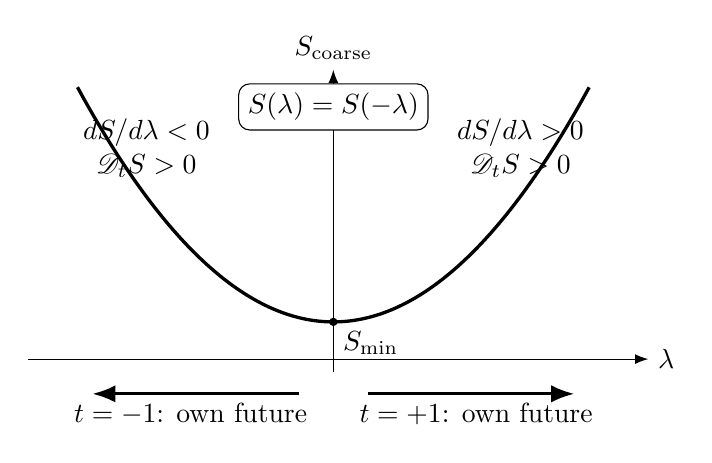
\begin{tikzpicture}[>=Latex,x=1.25cm,y=1.05cm]
 \draw[->] (-3.1,0)--(3.2,0) node[right] {$\lambda$};
 \draw[->] (0,-0.15)--(0,3.5) node[above] {$S_{\rm coarse}$};
 \draw[dashed] (0,0)--(0,3.15);
 \draw[very thick,domain=-2.6:2.6,samples=80,smooth]
 plot (\x,{0.42*\x*\x+0.45});
 \fill (0,0.45) circle (1.5pt);
 \node[below right] at (0,0.45) {$S_{\min}$};
 \draw[very thick,->] (-0.35,-0.42)--(-2.45,-0.42);
 \draw[very thick,->] (0.35,-0.42)--(2.45,-0.42);
 \node[below] at (-1.45,-0.42) {$t=-1$: own future};
 \node[below] at (1.45,-0.42) {$t=+1$: own future};
 \node[align=center] at (-1.9,2.55) {$dS/d\lambda<0$\\$\mathscr D_tS>0$};
 \node[align=center] at (1.9,2.55) {$dS/d\lambda>0$\\$\mathscr D_tS>0$};
 \node[draw,rounded corners,fill=white,align=center] at (0,3.05)
 {$S(\lambda)=S(-\lambda)$};
\end{tikzpicture}
\caption{A time-reflection-symmetric entropy profile can have opposite coordinate entropy gradients on its two oriented lifts while satisfying the same internal second law $\mathscr D_tS\ge0$ on both. The diagram represents two orientations of one time geometry; it does not require two independent universes.}
\label{fig:timesymmetricentropy}
\end{figure}

There is a finite-cover version of the same statement. Let $\mu$ be a $\mathsf D$-invariant measure on the orientation cover and let $\dot S(x)$ denote the coordinate entropy rate of the lifted history $x$, with
\begin{equation}
 \dot S(Dx)=-\dot S(x).
\end{equation}
Then pairwise cancellation gives
\begin{equation}\label{eq:signedentropycancel}
 \int \dot S\,d\mu=0,
\end{equation}
whereas if $\dot S(x)=t(x)\Sigma(x)$ with $\Sigma(\mathsf D x)=\Sigma(x)\ge0$, then
\begin{equation}\label{eq:orientedentropypositive}
 \int t\,\dot S\,d\mu=\int\Sigma\,d\mu\ge0.
\end{equation}
In this precise sense an exactly orientation-symmetric state can have no preferred signed entropy flux with respect to the arbitrary coordinate $\lambda$ while possessing positive thermodynamic production in each orientation's own future.

This is the mathematically clean residue of the old two-sided cosmological picture. It does not require two universes. The two orientations may be two lifts of one underlying state. For a $\mathsf D$-invariant lift measure, the phrase ``half the Universe goes toward $+\lambda$ and half toward $-\lambda$'' means equal weight on the two opposite orientation representatives, not two separately observable substances. The fixed-real-form construction itself does not assign a private thermodynamic entropy arrow to each elementary particle; the entropy statement is about paired coarse-grained histories.

For an FLRW description the same algebra appears in the pair $(H,\dot S)$. Under the passive reversal
\begin{equation}
 \lambda'=-\lambda,\qquad a'(\lambda')=a(-\lambda'),\qquad S'(\lambda')=S(-\lambda'),
\end{equation}
one has
\begin{equation}\label{eq:HSflip}
 H'(\lambda')=-H(-\lambda'),\qquad
 \frac{dS'}{d\lambda'}(\lambda')=-\frac{dS}{d\lambda}(-\lambda').
\end{equation}
Therefore, where neither factor vanishes,
\begin{equation}\label{eq:Xi}
 \boxed{\Xi=\sgn\!\left(H\frac{dS}{d\lambda}\right)}
\end{equation}
is invariant under simultaneous reversal. Expansion and coordinate entropy increase are separately orientation-sensitive labels; their relative alignment need not be.

What is not yet derived is the dynamical origin of a low-entropy reflection surface, or the claim that the microscopic $q,t$ cover necessarily organizes the entire cosmological state in the form of Corollary~\ref{cor:timesymentropy}. Those are physical hypotheses. The theorem is narrower and stronger: the second law itself can be written in an orientation-covariant form that is exactly compatible with time-reflection symmetry.

\subsection{The phase-level antecedent}\label{subsec:feynmanphase}
An orientation-covariant monotonicity statement of the form of Eq.~\eqref{eq:covariantSecondLaw} already appears in Feynman's positron paper, one level below thermodynamics. Discussing the Stueckelberg reading, he notes that the classical action, which is proper time, increases continuously along a trajectory, and that quantum mechanically this appears in the fact that the phase $|E_n|\,|t_2-t_1|$ always increases as the particle proceeds from one scattering point to the next~\cite{Feynman1949}.

The mechanism is the propagator prescription of that paper: positive-energy components propagate toward later coordinate time and negative-energy components toward earlier. Writing $t=\sgn(t_2-t_1)$ for the orientation of a segment, the prescription is $\sgn E_n=t$, so
\begin{equation}\label{eq:feynmanphasemonotone}
 E_n=t\,|E_n|,\qquad t_2-t_1=t\,|t_2-t_1|,\qquad
 \boxed{E_n(t_2-t_1)=t^2|E_n|\,|t_2-t_1|=|E_n|\,|t_2-t_1|.}
\end{equation}
The energy sign and the segment orientation reverse together and compensate, exactly as $q$ and $t$ do in $\chi=qt$. Equivalently, for the phase $\Phi(\lambda)=E_n\lambda$ along a segment parametrized by coordinate time $\lambda$,
\begin{equation}\label{eq:feynmanDt}
 \boxed{\mathscr D_t\Phi=t\,\frac{d\Phi}{d\lambda}=t\,E_n=|E_n|\ge0,}
\end{equation}
which is the operator $\mathscr D_t$ of Eq.~\eqref{eq:Dtdef} applied to phase rather than to coarse-grained entropy. The monotone quantity is oriented, not absolute, and its monotonicity is stated precisely because the backward segments belong to one continuous line.

Two consequences follow for the present programme. First, Theorem~\ref{thm:orientationsecondlaw} is not a new postulate but the coarse-grained analogue of a statement already required at the level of a single worldline. Second, the microscopic quantity known to be monotone along its own arrow is the accumulated phase, which by Theorem~\ref{thm:massphase} is $mc^2\tau/\hbar$. That is precisely the quantity Conjecture~\ref{conj:massclock} proposes the macroscopic record arrow inherits, so the conjecture proposes an inheritance between two monotone oriented quantities of the same type.

What Feynman's statement does not supply is the many-body step. Equation~\eqref{eq:feynmanphasemonotone} concerns phase along one line in an external potential, not stable records formed by a thermodynamic system. The entropy locking of Remark~\ref{rem:halfelectroncover} remains a separate dynamical hypothesis and is item (F9) of Appendix~\ref{app:falsify}.

\section{What an antimatter asymmetry would mean}
If antimatter is the relation of anti-alignment to a chosen record arrow, as in Section~\ref{subsec:arrows}, then an excess of matter over antimatter is an excess of alignment relative to our record arrow. That reframes the question without answering it.

Theorem~\ref{thm:quotient} changes one counting question but does not answer baryogenesis. If $(q,t)$ and $(-q,-t)$ are two lifts of the same relational state, then a $\mathsf D$-symmetric representative contains equal lift weight by Proposition~\ref{prop:equalliftweight}, but those two lifts must not be counted as independent reservoirs of matter and antimatter. With $Q_\star=-e$ both $++$ and $--$ belong to the electron class $\chi=+1$; the positron class is $\chi=-1$.

Laboratory antimatter is different because it is defined at fixed observer standards. A half flip changes $\chi$ and therefore changes the measured charge sign. The observed cosmic baryon asymmetry is likewise an asymmetry in relational charges and particle populations measured in our fixed macroscopic orientation. The diagonal quotient does not make that asymmetry disappear.

A complete cosmological model must still derive the baryon-to-photon ratio, CP-violating observables, nucleosynthesis and CMB constraints. The orientation construction supplies a different statement: an exactly time-reflected lift of the complete experiment is not an additional stockpile of missing antimatter merely because its $q$ and $t$ labels are both reversed. Whether a fundamental $\mathsf D$-symmetric state can generate the observed relational-sector asymmetry requires real dynamics, including the appropriate non-equilibrium and symmetry-violating ingredients.

\section{The recurring halves: an audit}
The programme was partly motivated by the conspicuous recurrence of halves, doubles, square roots and fourth roots. They must be sorted by origin.
\begin{center}
\begin{tabular}{>{\raggedright\arraybackslash}p{0.24\textwidth} >{\raggedright\arraybackslash}p{0.23\textwidth} >{\raggedright\arraybackslash}p{0.27\textwidth}}
\toprule
Structure & Exact factor & Status\\
\midrule
Spin cover & $\theta/2$, $2\pi\to-$, $4\pi\to+$ & topological\\
Dirac basis change & $1/\sqrt2$ & two-state normalization\\
Dirac rest clock & $\omega_Z=2\omega_C$ & representation/dynamics\\
Zitter amplitude & $a_Z=\bar\lambda_C/2$ & Dirac kinematics\\
Null momentum & $p=\lambda\bar\lambda$ & spinor square root\\
Massive momentum & $m^2=\det p$ & Lorentz invariant\\
Hodge split & $\Lambda^2=\Lambda^2_+\oplus\Lambda^2_-$ & orientation geometry\\
Celestial shadow & $\Delta\leftrightarrow2-\Delta$ & conformal representation\\
Diagonal $\mathbb Z_2$ gauge average & $1/2$ & normalized finite Haar measure\\
Normalized diagonal lift & $1/\sqrt2$ & Hilbert-space normalization after gauge average\\
Charged K\"ahler relative product & $Q=-IJ$, $Q^2=1$ & standard charged-field geometry\\
Normalized null basis & $1/\sqrt2$ & convention unless more shown\\
\bottomrule
\end{tabular}
\end{center}
The table is intentionally conservative. The appearance of the same integer is evidence only when an explicit morphism carries one structure into another.


\section{Grassmannian order four, the Pin lift, and transverse mass}\label{sec:grassmass}
The preceding mass--time statements acquire a geometric counterpart on the big cell of $\Gr(2,4)$. Write a two-plane in the standard chart as $[I\mid A]$, with
\begin{equation}
 A=\begin{pmatrix}a&b\\c&d\end{pmatrix},\qquad D=\det A=ad-bc\neq0,
\end{equation}
and let
\begin{equation}\label{eq:tau}
 \tau(A)=\frac{A\epsilon}{\det A},
 \qquad
 \epsilon=\begin{pmatrix}0&1\\-1&0\end{pmatrix}.
\end{equation}
In coordinates,
\begin{equation}
 \tau(a,b,c,d)=\frac{(-b,a,-d,c)}{D}.
\end{equation}
The following statements are exact algebraic identities. Their coordinate forms have also been machine-checked in Lean 4 in the accompanying Golden Physics verification library.

\begin{theorem}[Grassmannian order-four theorem]\label{thm:grassorder4}
For every point of the big cell with $D\neq0$,
\begin{equation}\label{eq:tau2tau4}
 \boxed{\tau^2=-\mathrm{id}},\qquad
 \boxed{\tau^4=\mathrm{id}}.
\end{equation}
Moreover $\tau^2(A)\neq A$ everywhere on the big cell, so the orbit has exact order four rather than merely order dividing four.
\end{theorem}
\begin{proof}
The determinant transforms as $D\mapsto D^{-1}$. Substituting the transformed coordinates into $\tau$ a second time gives $(-a,-b,-c,-d)$ exactly. Negation preserves $D$, so a second application of the same identity returns $(a,b,c,d)$. Equality $-A=A$ would force all four chart coordinates to vanish, contradicting $D\neq0$.
\end{proof}

The order-four map admits a decomposition that exposes a previously hidden piece of the googly geometry. Let
\begin{equation}\label{eq:grasscomplement}
 C(A)=-A^{-T}=\frac1D\begin{pmatrix}-d&c\\ b&-a\end{pmatrix},
 \qquad
 R=\begin{pmatrix}0&-1\\1&0\end{pmatrix}.
\end{equation}
For the graph plane $[I\mid A]$, the Pl\"ucker vector is
\begin{equation}
 p(A)=(1,c,d,-a,-b,D)
\end{equation}
in the ordered basis $(01,02,03,12,13,23)$. The Hodge/complement operation on $\Lambda^2\mathbb C^4$ sends
\begin{equation}
 (p_{01},p_{02},p_{03},p_{12},p_{13},p_{23})
 \longmapsto
 (p_{23},-p_{13},p_{12},p_{03},-p_{02},p_{01}),
\end{equation}
so
\begin{equation}
 *p(A)=(D,b,-a,d,-c,1).
\end{equation}
After projective normalization by $D^{-1}$, this is exactly the Pl\"ucker vector of $[I\mid C(A)]$. Thus $C$ is not an arbitrary rational map: it is the complementary-plane/annihilator operation induced by Hodge duality on the Klein quadric.

\begin{theorem}[Complement--quarter-turn factorization]\label{thm:tauFactor}
For every $A$ with $D\neq0$,
\begin{equation}\label{eq:taufactor}
 \boxed{\tau=R\circ C},
 \qquad C^2=I,
 \qquad R^2=-I,
 \qquad R^4=I,
 \qquad RC=CR.
\end{equation}
Consequently $\tau^2=-I$ and $\tau^4=I$.
\end{theorem}
\begin{proof}
Direct multiplication gives
\begin{equation}
 R C(A)=\frac1D\begin{pmatrix}-b&a\\-d&c\end{pmatrix}=\tau(A).
\end{equation}
The identity $C^2=I$ is the elementary double-annihilator relation on the invertible big cell, while $R^2=-I$. In $2\times2$ coordinates one checks $C(RA)=RC(A)$, hence $RC=CR$. The final two identities follow immediately. Each of these coordinate identities has an explicit Lean formulation in the accompanying verification development.
\end{proof}

This factorization is structurally useful. The involution $C$ carries the complementary-plane incidence geometry relevant to the googly problem, while the extra fixed factor $R$ carries the central sign responsible for the order-four lift. It would be premature to call $R$ the physical spin lift, but the decomposition identifies exactly where such a lift would have to enter.


\subsection{Global extension on the Klein quadric}

The denominator in Eq.~\eqref{eq:tau} is a chart normalization. Define on the Pl\"ucker carrier
\begin{equation}\label{eq:globalTK}
 \mathsf T_K(p_{01},p_{02},p_{03},p_{12},p_{13},p_{23})
 =
 (p_{23},-p_{03},p_{02},-p_{13},p_{12},p_{01})
\end{equation}
and let
\begin{equation}
 Q_K(p)=p_{01}p_{23}-p_{02}p_{13}+p_{03}p_{12}.
\end{equation}

\begin{theorem}[Global Klein order-four lift]\label{thm:globalKlein}
The map $\mathsf T_K$ obeys
\begin{align}
 Q_K(\mathsf T_Kp)&=Q_K(p),\\
 \det\mathsf T_K&=-1,\\
 \mathsf T_K^2(p)&=(p_{01},-p_{02},-p_{03},-p_{12},-p_{13},p_{23}),\\
 \mathsf T_K^4&=I.
\end{align}
Moreover, for every big-cell point with $D=\det A\neq0$,
\begin{equation}\label{eq:tauglobalprojective}
 \boxed{p(\tau A)=D^{-1}\mathsf T_K p(A).}
\end{equation}
Hence $\tau$ extends projectively across the full complex Klein quadric $Q_K=0$.
\end{theorem}

\begin{proof}
Substitution of Eq.~\eqref{eq:globalTK} into $Q_K$ gives
\begin{equation}
 p_{23}p_{01}-(-p_{03})p_{12}+p_{02}(-p_{13})=Q_K(p).
\end{equation}
The determinant and powers follow from the explicit signed permutation matrix. Finally
\begin{equation}
 \mathsf T_Kp(A)=(D,-d,c,b,-a,1),
\end{equation}
while
\begin{equation}
 p(\tau A)=\left(1,-\frac dD,\frac cD,\frac bD,-\frac aD,\frac1D\right),
\end{equation}
which is Eq.~\eqref{eq:tauglobalprojective}.
\end{proof}

\begin{remark}[Big-cell order versus global projective order]
Theorem~\ref{thm:grassorder4} remains exact on $D\neq0$, but projectivization changes the global orbit statement. Over $\mathbb C$,
\begin{equation}
 \chi_{\mathsf T_K}(t)=(t-1)(t+1)(t^2+1)^2.
\end{equation}
The two $\pm i$ eigenspaces are totally Klein-null, so their projectivizations lie on the complex Klein quadric and are fixed projectively. Thus ``every orbit has exact order four'' is a big-cell statement, not a statement about every complex projective point of the compactified quadric.
\end{remark}

The differential has an even sharper universal form. For a tangent variation $H$,
\begin{equation}\label{eq:dtau}
 d\tau_A(H)
 =\frac1D\left(H\epsilon-A\epsilon\,\operatorname{tr}(A^{-1}H)\right).
\end{equation}
Writing $H=AX$ gives
\begin{equation}\label{eq:universalL}
 d\tau_A(AX)=\frac1D A\,\mathcal L(X),
 \qquad
 \mathcal L(X)=X\epsilon-\epsilon\operatorname{tr}X.
\end{equation}
Thus, after the canonical identification $T_A\simeq M_2$ by left multiplication with $A^{-1}$, every point has the same tangent operator up to the single scalar factor $D^{-1}$.

\begin{theorem}[Universal differential and spectrum]\label{thm:grassdiff}
The universal operator of Eq.~\eqref{eq:universalL} obeys
\begin{equation}\label{eq:L4}
 \boxed{\mathcal L^4=I},
\end{equation}
and has characteristic polynomial
\begin{equation}\label{eq:Lchar}
 \chi_{\mathcal L}(t)=t^4-1.
\end{equation}
Consequently
\begin{equation}\label{eq:dtauchar}
 \boxed{\chi_{d\tau_A}(t)=t^4-D^{-4}},
\end{equation}
so over $\mathbb C$
\begin{equation}\label{eq:dtauspec}
 \operatorname{spec}(d\tau_A)
 =\left\{D^{-1},-D^{-1},iD^{-1},-iD^{-1}\right\},
\end{equation}
and every tangent eigenvalue has the same modulus,
\begin{equation}\label{eq:eigmod}
 \boxed{|\lambda|=|D|^{-1}}.
\end{equation}
\end{theorem}
\begin{proof}
In the coordinate basis $X=\bigl(\begin{smallmatrix}x_1&x_2\\x_3&x_4\end{smallmatrix}\bigr)$, Eq.~\eqref{eq:universalL} is an explicit linear map on four variables. Direct multiplication gives $\mathcal L^4=I$ and $\det(tI-\mathcal L)=t^4-1$. Equation~\eqref{eq:universalL} makes $d\tau_A$ similar to $D^{-1}\mathcal L$, which rescales all four eigenvalues and yields Eqs.~\eqref{eq:dtauchar}--\eqref{eq:eigmod}. Independently, if $N=D^2d\tau_A$ denotes the denominator-cleared Jacobian, the formally verified polynomial identity is $N^4=D^4I$; this is the same spectral statement with denominators removed.
\end{proof}

A useful correction follows from this theorem. The nonlinear identity $\tau^2=-\mathrm{id}$ does \emph{not} imply $(d\tau_A)^2=-I$ at one point. The chain rule instead gives
\begin{equation}\label{eq:chaincorrect}
 d\tau_{\tau(A)}\circ d\tau_A=-I.
\end{equation}
The two derivatives are taken at different points. This distinction removes a tempting but false ``Jacobian complex structure'' argument while preserving the exact order-four geometry.


\subsection{Null rulings and the conformally symplectic lift}

The differential simplifies drastically on a null tangent. Write a rank-one tangent as
\begin{equation}
 H=u\,v^T,\qquad u,v\in\mathbb C^2,
\end{equation}
and set $x=A^{-1}u$. The two-dimensional identity
\begin{equation}
 x v^T\epsilon-\epsilon(v^Tx)=-\epsilon v x^T
\end{equation}
turns Eq.~\eqref{eq:dtau} into the factorization
\begin{equation}\label{eq:nullfactor}
 \boxed{
 d\tau_A(uv^T)
 =
 \left(-D^{-1}A\epsilon v\right)
 \left(A^{-1}u\right)^T.}
\end{equation}
Thus $d\tau$ exchanges the two spinor factors of the rank-one tangent cone.

\begin{theorem}[Order four on the spinor rulings]\label{thm:rulingswap}
Define
\begin{equation}
 F_A(u,v)=\left(-D^{-1}A\epsilon v,\;A^{-1}u\right).
\end{equation}
If $A'=\tau(A)$, then
\begin{equation}\label{eq:Fcompose}
 \boxed{F_{A'}F_A(u,v)=(u,-v).}
\end{equation}
Consequently the induced rank-one matrix satisfies
\begin{equation}
 d\tau_{\tau(A)}d\tau_A(uv^T)=-uv^T,
\end{equation}
whereas its projective null direction has order two.
\end{theorem}

\begin{proof}
Since $\det A'=D^{-1}$ and $A'=D^{-1}A\epsilon$, direct substitution gives
\begin{align}
 -(\det A')^{-1}A'\epsilon(A^{-1}u)&=u,\\
 (A')^{-1}\left(-D^{-1}A\epsilon v\right)&=-v.
\end{align}
Equation~\eqref{eq:nullfactor} then gives the matrix statement.
\end{proof}

There is also a canonical bilinear structure behind this exchange. On
$\mathbb C^2\oplus\mathbb C^2$ let
\begin{equation}
 \Omega=
 \begin{pmatrix}\epsilon&0\\0&\epsilon\end{pmatrix},
 \qquad
 F_A=
 \begin{pmatrix}
 0&-D^{-1}A\epsilon\\
 A^{-1}&0
 \end{pmatrix}.
\end{equation}
Using $M^T\epsilon M=(\det M)\epsilon$ for every $2\times2$ matrix,
\begin{equation}\label{eq:confsympl}
 \boxed{F_A^T\Omega F_A=D^{-1}\Omega.}
\end{equation}
Hence, after choosing a square root of $D$, the rescaled map
\begin{equation}
 \widehat F_A=D^{1/2}F_A
\end{equation}
is symplectic. This is the precise classical datum required for a metaplectic/Fourier lift; no quantization claim follows merely from Eq.~\eqref{eq:confsympl}.


\subsection{The square-root lift has nontrivial holonomy}\label{subsec:sqrtmonodromy}
The square root in the preceding paragraph is not a harmless local notation. On the invertible big cell
\begin{equation}
 \mathcal U=GL_2(\mathbb C)=\{A:\det A\neq0\},
\end{equation}
define the determinant square-root cover
\begin{equation}\label{eq:sqrtcover}
 \widetilde{\mathcal U}
 =\{(A,s)\in\mathcal U\times\mathbb C^*:s^2=\det A\},
 \qquad
 \pi(A,s)=A,
\end{equation}
with deck transformation $\delta(A,s)=(A,-s)$. The symplectic lift is naturally a function on $\widetilde{\mathcal U}$,
\begin{equation}
 \widehat F_{(A,s)}=sF_A,
\end{equation}
rather than a single-valued function of $A$ alone.

\begin{theorem}[Determinant-winding monodromy]\label{thm:detmonodromy}
Let $A:[0,1]\to GL_2(\mathbb C)$ be a closed loop and let
\begin{equation}
 n=\operatorname{wind}(\det A,0)\in\mathbb Z.
\end{equation}
A continuous lift $s(t)$ satisfying $s(t)^2=\det A(t)$ returns as
\begin{equation}\label{eq:monodromysign}
 \boxed{s(1)=(-1)^n s(0).}
\end{equation}
In particular the explicit loop
\begin{equation}\label{eq:generatorloop}
 A(\theta)=\begin{pmatrix}e^{i\theta}&0\\0&1\end{pmatrix},
 \qquad 0\le\theta\le2\pi,
\end{equation}
has $A(2\pi)=A(0)$ but a lift beginning at $s(0)=1$ ends at $s(2\pi)=-1$.
\end{theorem}
\begin{proof}
Write continuously along the loop
\begin{equation}
 \det A(t)=r(t)e^{i\phi(t)},\qquad r(t)>0,
\end{equation}
with $\phi(1)-\phi(0)=2\pi n$. A continuous square root is
\begin{equation}
 s(t)=\sqrt{r(t)}e^{i\phi(t)/2},
\end{equation}
so
\begin{equation}
 s(1)=e^{i\pi n}s(0)=(-1)^n s(0).
\end{equation}
For Eq.~\eqref{eq:generatorloop}, $\det A=e^{i\theta}$ and $s=e^{i\theta/2}$ gives the stated sign change directly.
\end{proof}

This resolves an important observability issue. The absolute choice $s\leftrightarrow-s$ is a local lift label: it changes neither $A$ nor the projective null direction. Nevertheless the cover is not globally trivial. Its parity of winding is a gauge-invariant relational datum of a closed history.

\begin{corollary}[Interference signature of the lift]\label{cor:liftinterference}
Suppose a coherent physical amplitude carries the nontrivial one-dimensional representation of the deck group, so that $\delta$ acts by $-1$. For two histories with the same endpoints whose determinant windings differ by $n$, the relative lift phase is
\begin{equation}\label{eq:relativeholonomy}
 \boxed{H_{12}=(-1)^n.}
\end{equation}
Thus an odd difference of winding changes the interference cross term by a sign even though no local measurement can assign an absolute sheet label.
\end{corollary}
\begin{proof}
Transport along each history lifts to a deck element $(-1)^{n_i}$. Their relative action is $(-1)^{n_2-n_1}$, which is Eq.~\eqref{eq:relativeholonomy}.
\end{proof}

Corollary~\ref{cor:liftinterference} is a conditional physical prediction, not yet a claim that an available laboratory control parameter traces Eq.~\eqref{eq:generatorloop}. The exact result is the nontrivial monodromy of the geometric square-root cover. To make it experimental one must identify a physical adiabatic cycle whose state really carries this lift. This is the correct sense in which the fold can be observable without making either absolute sheet physical.

The search for that cycle is more constrained than it first appears, because the winding in Theorem~\ref{thm:detmonodromy} is blind to the Lorentz group.

\begin{proposition}[Lorentz loops have zero determinant winding]\label{prop:lorentznowind}
On complexified Minkowski space let the spin group act on the matrix chart by
\begin{equation}\label{eq:lorentzchart}
 A\longmapsto L\,A\,R^T,\qquad L,R\in SL(2,\mathbb C).
\end{equation}
On the Hermitian Minkowski real slice this reduces to $A\mapsto LAL^\dagger$. In either case $\det A$ is invariant. Consequently every closed path obtained by acting on a fixed $A$ with Lorentz transformations has $\operatorname{wind}(\det A,0)=0$, and the determinant-square-root lift returns unchanged.
\end{proposition}
\begin{proof}
$\det(LAR^T)=\det L\,\det A\,\det R=\det A$. On the real slice, $\det(LAL^\dagger)=|\det L|^2\det A=\det A$. A constant nonzero determinant has zero winding.
\end{proof}

\begin{corollary}[The determinant cover is not the Lorentz spin cover]\label{cor:notspincover}
A $2\pi$ spatial rotation, and more generally any closed Lorentz orbit of a fixed chart point, does not realize the deck element of Theorem~\ref{thm:detmonodromy}. The determinant square-root cover and the Lorentz spin double cover are covers of different base spaces; familiar $4\pi$ spin-rotation experiments do not measure determinant winding.
\end{corollary}

This removes the most natural wrong candidate and identifies a non-Lorentz cycle explicitly. In the position chart $A=x^\mu\sigma_\mu$ one has
\begin{equation}\label{eq:detisinterval}
 \boxed{\det A=x\cdot x,}
\end{equation}
so the zero locus is the complexified light cone.

\begin{proposition}[An explicit light-cone meridian]\label{prop:lightconemeridian}
Fix $0<\rho<1$ and, in mostly-minus convention, set
\begin{equation}
 x^1(\theta)=1,\qquad
 x^0(\theta)=\sqrt{1+\rho e^{i\theta}},\qquad
 x^2(\theta)=x^3(\theta)=0,\qquad 0\le\theta\le2\pi,
\end{equation}
where the square root is continued from $\theta=0$. Then $x(2\pi)=x(0)$,
\begin{equation}
 x(\theta)\cdot x(\theta)=\rho e^{i\theta},
\end{equation}
and the determinant has winding one. The lift $s^2=\det A$ therefore returns with $s(2\pi)=-s(0)$.
\end{proposition}
\begin{proof}
The circle $1+\rho e^{i\theta}$ does not enclose the origin, so its square root has a closed continuous branch. Substitution gives $x^2=\rho e^{i\theta}$, whose winding is one, and Theorem~\ref{thm:detmonodromy} gives the sign.
\end{proof}

The same light-cone locus controls the analytic structure of the massive scalar propagator. In natural units and mostly-minus convention,
\begin{equation}\label{eq:massivepropbranch}
 \Delta_F(x)=\frac{m}{4\pi^2}
 \frac{K_1\!\left(m\sqrt{-x^2+i0}\right)}
 {\sqrt{-x^2+i0}}.
\end{equation}
This makes $x^2=0$ a common branch locus, but it does not identify the square-root deck sign with the full propagator monodromy: the Bessel function and the $i0$ boundary value also contribute. The precise theorem target is therefore an intertwining of the deck local system with the discontinuity local system used in the shadow-cut construction, not a comparison of branch points alone.

Separately, the pullback constructed below identifies the determinant square-root cover with the transverse $\mathrm{Spin}(2)$ cover, and the free Dirac evolution supplies a representation of that transverse cover. One transverse-vector circuit occurs in proper time $\pi/\omega_C$, exactly when the spinor acquires $-1$. The light-cone meridian and the Compton circuit are thus two pullbacks of the universal map $z\mapsto z^2$ under different base maps. No theorem here identifies them as the same physical loop, and neither is a Lorentz rotation.

\subsection{The \texorpdfstring{$8=4+4$}{8=4+4} Pin carrier and an order-four Fourier kernel}

The global map $\mathsf T_K$ has determinant $-1$, so it belongs to the disconnected component of $O(6,\mathbb C)$. The Pin covering therefore has an odd lift exchanging the two half-spin representations. In six complex dimensions
\begin{equation}\label{eq:cl6spin}
 \mathrm{Cl}_6(\mathbb C)\simeq M_8(\mathbb C),\qquad
 S=\Lambda^\bullet\mathbb C^3=S_+\oplus S_-,
 \qquad
 \dim_\mathbb C S_\pm=4.
\end{equation}
Thus the natural full carrier is eight-dimensional, not because the four-dimensional Dirac representation has been arbitrarily doubled, but because the six-dimensional Klein/Clifford geometry has two four-dimensional chiral half-spin modules.

In the Fock basis
\begin{equation}
 S_+=(1,e_{12},e_{13},e_{23}),\qquad
 S_-=(e_1,e_2,e_3,e_{123}),
\end{equation}
one may choose the two chiral blocks
\begin{equation}\label{eq:pinblocks}
 M_+=
 \begin{pmatrix}
 1&0&0&0\\
 0&0&1&0\\
 0&-1&0&0\\
 0&0&0&1
 \end{pmatrix},
 \qquad
 M_-=
 \begin{pmatrix}
 -1&0&0&0\\
 0&0&-1&0\\
 0&1&0&0\\
 0&0&0&-1
 \end{pmatrix}.
\end{equation}
After the corresponding signed permutation identifying the Witt basis of
$\mathbb C^3\oplus(\mathbb C^3)^*$ with the Pl\"ucker basis, this is a Pin representative of Eq.~\eqref{eq:globalTK}. Direct multiplication gives
\begin{equation}\label{eq:pinsquare}
 M_-M_+=M_+M_-=
 \Gamma:=\operatorname{diag}(-1,1,1,-1),
 \qquad \Gamma^2=I.
\end{equation}
Therefore the odd $8\times8$ operator
\begin{equation}
 \widetilde{\mathsf T}_K=
 \begin{pmatrix}0&M_-\\M_+&0\end{pmatrix}
\end{equation}
satisfies
\begin{equation}\label{eq:pinorder4}
 \boxed{\widetilde{\mathsf T}_K^{\,2}
 =\operatorname{diag}(\Gamma,\Gamma),\qquad
 \widetilde{\mathsf T}_K^{\,4}=I.}
\end{equation}

The same finite algebra can be put into a Fourier kernel. With the Chevalley-pairing convention
\begin{equation}
 B_T=
 \begin{pmatrix}
 0&0&0&-1\\
 0&-1&0&0\\
 0&0&-1&0\\
 1&0&0&0
 \end{pmatrix},
 \qquad \det B_T=1,
\end{equation}
one finds
\begin{equation}
 -B_T^{-1}B_T^T=-\Gamma.
\end{equation}
For Schwartz data on a compatible real slice define
\begin{equation}\label{eq:GTfourier}
 (\mathcal G_Tf)(Z)
 =
 \frac1{(2\pi)^2}\int_{\mathbb R^4}
 e^{-iZ^TB_TW}f(W)\,d^4W.
\end{equation}
Fourier inversion gives
\begin{equation}\label{eq:GTsquare}
 \boxed{\mathcal G_T^2f(Z)=f(-\Gamma Z),\qquad
 \mathcal G_T^4=I.}
\end{equation}
For homogeneous twistor distributions $f(tZ)=t^k f(Z)$ with Penrose degree
$k=2h-2$,
\begin{equation}
 f(-\Gamma Z)=(-1)^k f(\Gamma Z)=(-1)^{2h}f(\Gamma Z).
\end{equation}
The boson/fermion central sign is therefore inherited from homogeneity rather than inserted by hand.

The degree reflection $k\mapsto-k-4$ must still be interpreted side-aware. Cross-side Fourier maps a twistor representative to a dual-twistor representative; calling this a physical helicity reversal requires an additional identification of the two sides. What is unconditional is the degree reflection itself. Brown, Gowdy and Spence prove that Lorentzian Fourier transformation followed by the appropriate celestial Mellin transform realizes the boundary shadow transform~\cite{BrownGowdySpence2023}. Thus the order-four Pin/Fourier construction supplies an upstairs lift of the same Weyl reflection whose boundary labels are
\begin{equation}
 (\Delta,J)\longmapsto(2-\Delta,-J),
\end{equation}
without equating the geometric Pin map, the Fourier operator, the anti-linear Hilbert reflection, and bare shadow.


\subsection{Doubled Lorentzian parent and the transverse mass plane}

Return now to the doubled carrier
\begin{equation}
 W=V_1\oplus V_2,\qquad V_1\simeq V_2\simeq\mathbb R^{3,1},
\end{equation}
with product metric
\begin{equation}
 G((x_1,x_2),(y_1,y_2))=g(x_1,y_1)+g(x_2,y_2).
\end{equation}
Its real signature is $(6,2)$. Define
\begin{equation}\label{eq:J8}
 \mathcal J(x_1,x_2)=(x_2,-x_1).
\end{equation}
Then
\begin{equation}\label{eq:J8powers}
 \boxed{\mathcal J^2=-I,\qquad \mathcal J^4=I.}
\end{equation}
The diagonal and anti-diagonal Lorentzian four-planes
\begin{equation}
 L_+=\{(x,x)\},\qquad L_-=\{(x,-x)\}
\end{equation}
are exchanged by $\mathcal J$ up to the central sign.

\begin{theorem}[Canonical doubled quarter-turn]\label{thm:doubledquarter}
The map $\mathcal J$ is $G$-orthogonal, has order four, and satisfies
\begin{equation}
 L_+\xrightarrow{\mathcal J}L_-\xrightarrow{\mathcal J}-L_+.
\end{equation}
\end{theorem}
\begin{proof}
Orthogonality follows from
\[
G(\mathcal J(x_1,x_2),\mathcal J(y_1,y_2))
=g(x_2,y_2)+g(x_1,y_1)
=G((x_1,x_2),(y_1,y_2)).
\]
The power identities and the action on $L_\pm$ are immediate.
\end{proof}

This order four exists before introducing spinors. It is the same exchange-plus-relative-sign algebra that appeared independently in the finite spin-center construction, but no physical identification of the two operations is needed for either theorem.

To recover the Klein signature, choose a positive-definite two-plane $E\subset W$ and let
\begin{equation}
 K=E^\perp.
\end{equation}
Then
\begin{equation}\label{eq:6242}
 \boxed{W^{6,2}=K^{4,2}\oplus E^{2,0}.}
\end{equation}
A concrete realization starts with $L_+$ as the observed Lorentzian four-plane and chooses in $L_-$ one spacelike and one timelike direction for the additional $(1,1)$ conformal pair; the two remaining relative spatial directions form $E$. This choice is extra structure and is not claimed to be canonical.

Write the $E$ coordinates as $(u,v)$ and let $P\in K$. The eight-dimensional quadratic form is
\begin{equation}\label{eq:Q8}
 \boxed{Q_8(P,u,v)=Q_K(P)+u^2+v^2.}
\end{equation}
Hence an eight-dimensional null vector satisfies
\begin{equation}\label{eq:offklein}
 \boxed{Q_K(P)=-(u^2+v^2).}
\end{equation}
At $u=v=0$ the six-dimensional component lies on the Klein null cone, whose complex projectivization is the Klein quadric $Q^4\simeq\Gr(2,4)$. A nonzero transverse radius therefore moves $P$ off the Klein quadric while the full eight-dimensional vector remains null.

This observation corrects an earlier target in the present programme. Every genuine Pl\"ucker point obeys
\begin{equation}
 Q_K(p(A))=0
\end{equation}
identically, while the chart determinant $D=\det A$ varies over the big cell. Therefore $D$ cannot, by itself, be the invariant normal distance from the Klein quadric. The tentative law $|D|=m/\mu$ is retired. The exact statement retained from Theorem~\ref{thm:grassdiff} is only that $D$ controls the scale of the chart differential. If a dimensionful reference scale $\mu$ is chosen, the natural dimensionless transverse radius is instead
\begin{equation}\label{eq:transmassdict}
 \rho=\sqrt{u^2+v^2}=\frac{m}{\mu},
 \qquad
 Q_K(P)=-\left(\frac{m}{\mu}\right)^2.
\end{equation}
Equation~\eqref{eq:transmassdict} is a geometric mass dictionary until the physical section is specified; the next theorem supplies an independent dynamical reason for reading a conserved relative-momentum norm as four-dimensional rest mass.

\begin{remark}[Projective-scale caveat]\label{rem:projectivescale}
The full null cone $Q_8=0$ is homogeneous. Therefore the absolute radius $|q|$ is not itself a projective invariant: $(P,q)$ and $(\lambda P,\lambda q)$ determine the same projective null direction. A physical mass appears only after an affine scale is fixed, represented above by $\mu$, or after a compensator or boundary condition supplies the equivalent information. What is invariant before that choice is the ratio encoded by the selected section. Thus the doubled geometry explains where a mass coordinate can live and how it breaks the six-dimensional Klein-null condition; it does not create a dimensionful scale from projective geometry alone.
\end{remark}

\subsection{Null-parent reduction to the massive worldline}

There is a direct classical reduction that does not use the Grassmannian chart determinant or the choice of $E$. Work in the orthogonal diagonal/relative decomposition $W=L_+\oplus L_-$, let $x\in L_+$ and $y\in L_-$, and consider the first-order massless action
\begin{equation}\label{eq:nullparentaction}
 S_0=\int d\lambda\left[
 p\cdot\dot x+k\cdot\dot y-\frac e2(p^2+k^2)
 \right].
\end{equation}
The relative coordinate is cyclic, so $k$ is conserved.

\begin{theorem}[Null-parent mass reduction]\label{thm:nullparentmass}
Fix a sector with spacelike relative momentum
\begin{equation}
 k^2=m^2c^2,\qquad m>0.
\end{equation}
Routh reduction of Eq.~\eqref{eq:nullparentaction} at fixed $k$ gives
\begin{equation}
 S_{\rm red}
 =\int d\lambda\left[
 p\cdot\dot x-\frac e2(p^2+m^2c^2)
 \right].
\end{equation}
Eliminating $p$ and $e$ gives the standard massive four-dimensional action
\begin{equation}\label{eq:massiveactionfromnull}
 \boxed{S_{\rm red}=-mc^2\int d\tau.}
\end{equation}
Along the parent equations of motion,
\begin{equation}\label{eq:hiddenphase}
 p\cdot dx=-mc^2d\tau,\qquad
 dy^2=c^2d\tau^2,\qquad
 k\cdot dy=+mc^2d\tau.
\end{equation}
Thus the observed proper-time phase is the negative of the relative canonical phase along the null parent trajectory.
\end{theorem}

\begin{proof}
Routh reduction subtracts the fixed cyclic term $k\cdot\dot y$ and inserts $k^2=m^2c^2$. Variation gives $\dot x=ep$ and the constraint $p^2=-m^2c^2$. Eliminating $p$ and the einbein gives Eq.~\eqref{eq:massiveactionfromnull}. The parent equation $\dot y=ek$ yields $dy^2=e^2m^2c^2d\lambda^2$, while $dx^2=-e^2m^2c^2d\lambda^2$, hence $dy^2=-dx^2=c^2d\tau^2$. Finally $p\cdot dx=ep^2d\lambda=-mc^2d\tau$ and $k\cdot dy=ek^2d\lambda=+mc^2d\tau$.
\end{proof}

In terms of momenta of the original two Lorentzian copies,
\begin{equation}
 p=\frac{p_1+p_2}{\sqrt2},\qquad
 k=\frac{p_1-p_2}{\sqrt2}.
\end{equation}
The parent null condition is $p_1^2+p_2^2=p^2+k^2=0$. Hence
\begin{equation}\label{eq:relmass}
 \boxed{
 m^2c^2=k^2
 =\frac12(p_1-p_2)^2
 =-p^2
 =-\frac12(p_1+p_2)^2.}
\end{equation}
Thus, within the null-parent model, four-dimensional rest mass is the invariant magnitude of the spacelike relative momentum between the two $3+1$ copies.

\begin{theorem}[Massless doubled field to massive Klein--Gordon field]\label{thm:kgnullparent}
Let $\Phi(x,y)$ satisfy the massless equation
\begin{equation}
 (\Box_x+\Box_y)\Phi=0.
\end{equation}
For a separated relative-momentum mode
\begin{equation}
 \Phi(x,y)=e^{ik\cdot y/\hbar}\varphi(x),\qquad k^2=m^2c^2,
\end{equation}
the four-dimensional factor obeys
\begin{equation}
 \boxed{\left(\Box_x-\frac{m^2c^2}{\hbar^2}\right)\varphi=0}
\end{equation}
in the space-positive convention of this subsection.
\end{theorem}
\begin{proof}
The relative d'Alembertian acts on the plane wave by $\Box_y e^{ik\cdot y/\hbar}=-(k^2/\hbar^2)e^{ik\cdot y/\hbar}$.
\end{proof}

The Dirac linearization can be performed directly on the full doubled Clifford algebra as well. Return here to the mostly-minus convention $\eta=\operatorname{diag}(+,-,-,-)$ used in the earlier Dirac sections, and let $\Gamma_x^\mu$ and $\Gamma_y^\mu$ be two mutually anticommuting copies of the four-dimensional Clifford generators,
\begin{equation}
 \{\Gamma_x^\mu,\Gamma_x^\nu\}=2\eta^{\mu\nu},\quad
 \{\Gamma_y^\mu,\Gamma_y^\nu\}=2\eta^{\mu\nu},\quad
 \{\Gamma_x^\mu,\Gamma_y^\nu\}=0.
\end{equation}

\begin{theorem}[Direct doubled-Dirac mass reduction]\label{thm:doubleddirac}
Let $k^\mu=mc\,n^\mu$ with $n^2=-1$ and define
\begin{equation}
 N=\Gamma_y(n),\qquad
 \gamma_{\rm eff}^{\mu}=N\Gamma_x^\mu.
\end{equation}
Then
\begin{equation}
 N^2=-I,\qquad
 \{\gamma_{\rm eff}^{\mu},\gamma_{\rm eff}^{\nu}\}=2\eta^{\mu\nu}I.
\end{equation}
Consequently the massless doubled equation
\begin{equation}
 (\Gamma_x\cdot p+\Gamma_y\cdot k)\Psi=0
\end{equation}
implies
\begin{equation}
 \boxed{(\gamma_{\rm eff}\cdot p-mc)\Psi=0.}
\end{equation}
On either complex eight-dimensional Weyl module of the parent Clifford algebra, the resulting representation of the complex four-dimensional Clifford algebra is reducible as two four-component Dirac modules.
\end{theorem}
\begin{proof}
Since $N^2=n^2I=-I$ and $N$ anticommutes with every $\Gamma_x^\mu$,
\[
\{N\Gamma_x^\mu,N\Gamma_x^\nu\}
=-N^2\{\Gamma_x^\mu,\Gamma_x^\nu\}
=2\eta^{\mu\nu}I.
\]
Multiplying the parent equation from the left by $N$ gives the result. Since the complex four-dimensional Clifford algebra is $M_4(\mathbb C)$, an eight-dimensional complex module is the direct sum of two irreducible four-dimensional modules.
\end{proof}

The last sentence is an obstruction as much as a result. The naive doubled Dirac reduction produces an internal twofold degeneracy. A single observed four-component Dirac carrier therefore requires one additional commuting projector, gauge condition or dynamical selection rule. A noncompact relative momentum space also supplies a continuum of possible $k^2$ and therefore a continuum of effective masses. Reproducing a discrete particle spectrum requires an additional spectral mechanism. Nothing in the null reduction alone selects the Standard-Model masses.

The theorem is a dimensional reduction, not yet a confinement theorem. It says that if the relative coordinates are quotiented, gauge, unobserved or otherwise removed at fixed relative momentum, then their conserved norm is observed as rest mass. It does not explain why a physical observer cannot access $y$. That is now the precise dynamical question behind the older phrase ``dimensional confinement by mass.'' The less misleading term is \emph{dimensional folding}: the parent coordinates remain part of the full geometry while their relative momentum, phase and spinorial locking descend as internal data of the effective four-dimensional description.

The proper-time relation is nevertheless exact and sharpens the mass--clock theorem. In the null parent the canonical one-form vanishes on shell by cancellation,
\begin{equation}
 p\cdot dx+k\cdot dy=0,
\end{equation}
while the reduced observer retains one half of that relation as the massive action phase. No photon rest frame and no attribution of an observer perspective to a null worldline is required.

\subsection{Eight-component Clifford factorization of the transverse mass shell}

The spinor algebra factorizes the same enlarged quadratic form. Complexify $K$ and let
\begin{equation}
 c_+(P):S_+\to S_-,
 \qquad
 c_-(P):S_-\to S_+
\end{equation}
be the four-component Klein Clifford maps. They obey
\begin{equation}\label{eq:cliffk}
 c_-(P)c_+(P)=c_+(P)c_-(P)=-Q_K(P)I_4.
\end{equation}
Introduce
\begin{equation}
 \zeta_\perp=u+iv,\qquad |\zeta_\perp|^2=u^2+v^2.
\end{equation}
On $S_+\oplus S_-$ define
\begin{equation}\label{eq:Dpm}
 \mathcal D_+(P,\zeta_\perp)=
 \begin{pmatrix}
 -\zeta_\perp I_4&c_-(P)\\
 c_+(P)&-\bar\zeta_\perp I_4
 \end{pmatrix},
 \qquad
 \mathcal D_-(P,\zeta_\perp)=
 \begin{pmatrix}
 \bar\zeta_\perp I_4&c_-(P)\\
 c_+(P)&\zeta_\perp I_4
 \end{pmatrix}.
\end{equation}

\begin{theorem}[Eight-component factorization]\label{thm:8factor}
The two first-order symbols factor the extended quadratic form exactly:
\begin{equation}\label{eq:8factor}
 \boxed{
 \mathcal D_-\mathcal D_+
 =
 \mathcal D_+\mathcal D_-
 =
 -\bigl(Q_K(P)+|\zeta_\perp|^2\bigr)I_8.}
\end{equation}
Consequently the extended null condition $Q_8=0$ is exactly the quadratic shell factorized by an eight-component first-order system.
\end{theorem}
\begin{proof}
Multiply the block matrices. The off-diagonal blocks cancel because $\zeta_\perp$ is scalar, while each diagonal block is $-|\zeta_\perp|^2I_4+c_-c_+$ or its $c_+c_-$ counterpart, and Eq.~\eqref{eq:cliffk} applies.
\end{proof}

Because $\mathcal D_\pm$ are real-linear in the eight ambient coordinates, polarizing Eq.~\eqref{eq:8factor} gives the full chiral Clifford relation. On shell, $\mathcal D_+\Psi=0$ for $\Psi=(Z,W)$ is
\begin{equation}\label{eq:massivelock}
 c_-(P)W=\zeta_\perp Z,\qquad
 c_+(P)Z=\bar\zeta_\perp\,W.
\end{equation}
At $\zeta_\perp=0$ and $Q_K=0$ these reduce to the independent massless incidence equations
\begin{equation}
 c_-(P)W=0,\qquad c_+(P)Z=0.
\end{equation}
For $\zeta_\perp\neq0$, either four-component half determines the other, for example
\begin{equation}
 W=\bar\zeta_\perp^{-1}c_+(P)Z,
\end{equation}
and the remaining equation follows automatically from $-Q_K=|\zeta_\perp|^2$. Thus nonzero transverse radius does not delete components; it locks the two chiral halves that were independent on the Klein cone.

The phase of $\zeta_\perp$ is relative rather than radial. Equation~\eqref{eq:massivelock} is covariant under
\begin{equation}
 \zeta_\perp\mapsto e^{-i\alpha}\zeta_\perp,\qquad
 Z\mapsto e^{i\alpha/2}Z,\qquad
 W\mapsto e^{-i\alpha/2}W.
\end{equation}
Hence $|\zeta_\perp|$ is the invariant of the free locking algebra, while the transverse $SO(2)$ angle is a chiral relative phase. A quarter-turn $\zeta_\perp\mapsto i\zeta_\perp$ has order four on the transverse vector but order eight on its genuine $\mathrm{Spin}(2)$ lift; projectively the central spinor sign reduces the order again to four. In particular a full circuit $\zeta_\perp=\rho e^{i\theta}$ with $\theta:0\to2\pi$ returns the transverse vector to itself while multiplying both half-spinor factors by the central sign $-1$. The determinant square-root cover and this transverse spin cover are in fact the same double cover after the natural determinant-phase map.

\subsection{The determinant, transverse, and Dirac covers are explicitly intertwined}\label{subsec:threecover}
Write
\begin{equation}\label{eq:detphase}
 d(A)=\frac{\det A}{|\det A|}\in U(1),\qquad A\in GL_2(\mathbb C),
\end{equation}
and identify the oriented transverse unit circle with $SO(2)\simeq U(1)$. We use
\begin{equation}
 \mathrm{Spin}(2)\simeq U(1),\qquad \varpi(z)=z^2
\end{equation}
for the standard double cover. Fix a nonzero transverse radius $\rho$ and define
\begin{equation}\label{eq:pullbackspincover}
 \mathcal P_\rho=
 \left\{(A,\zeta_\perp,z):
 A\in GL_2(\mathbb C),\ |\zeta_\perp|=\rho,\ \zeta_\perp=\rho\,d(A),\ z\in U(1),\ z^2=\frac{\zeta_\perp}{\rho}
 \right\}.
\end{equation}

\begin{theorem}[Determinant--transverse spin-cover equivalence]\label{thm:detspincover}
The determinant square-root cover of Eq.~\eqref{eq:sqrtcover} is isomorphic, as a principal $\mathbb Z_2$ cover, to the pullback transverse spin cover $\mathcal P_\rho$. An explicit isomorphism is
\begin{equation}\label{eq:PhiCover}
 \boxed{
 \Phi_\rho(A,s)=
 \left(A,\rho\frac{\det A}{|\det A|},\frac{s}{|s|}\right).}
\end{equation}
Its inverse is
\begin{equation}\label{eq:PhiCoverInv}
 \boxed{
 \Phi_\rho^{-1}(A,\zeta_\perp,z)=
 \left(A,\sqrt{|\det A|}\,z\right).}
\end{equation}
Moreover the deck transformations are intertwined:
\begin{equation}
 (A,s)\mapsto(A,-s)
 \quad\Longleftrightarrow\quad
 (A,\zeta_\perp,z)\mapsto(A,\zeta_\perp,-z).
\end{equation}
Consequently determinant winding, transverse-vector winding and the central spin-lift sign have the same parity.
\end{theorem}
\begin{proof}
Since $s^2=\det A$, taking absolute values gives $|s|^2=|\det A|$. Therefore
\begin{equation}
 \left(\frac{s}{|s|}\right)^2
 =\frac{s^2}{|s|^2}
 =\frac{\det A}{|\det A|}
 =d(A),
\end{equation}
so Eq.~\eqref{eq:PhiCover} lands in $\mathcal P_\rho$. Conversely, if $z^2=d(A)$, then
\begin{equation}
 \left(\sqrt{|\det A|}\,z\right)^2
 =|\det A|d(A)=\det A,
\end{equation}
which proves Eq.~\eqref{eq:PhiCoverInv}. The two maps are inverse, and $s\mapsto-s$ is exactly $z\mapsto-z$. The winding statement follows because $\zeta_\perp/\rho=d(A)$.
\end{proof}

This result removes the first of the three former intertwiner gaps. Up to the choice of orientation of the transverse two-plane, the determinant phase is the $SO(2)$ vector angle and its square root is the $\mathrm{Spin}(2)$ half-angle. No identification with laboratory antimatter has been made: the deck element $z\mapsto-z$ is central and multiplies every spinor component by the same sign.

The remaining step to the standard free Dirac carrier is also explicit. Let $p$ be future timelike with
\begin{equation}
 p^2=m^2c^2,
\end{equation}
use the mostly-minus Clifford convention, and define the covariant Dirac involution
\begin{equation}\label{eq:Bp}
 B_p=\frac{\slashed p}{mc},\qquad B_p^2=I_4,
\end{equation}
with spectral projectors
\begin{equation}\label{eq:PpmDirac}
 P_\pm(p)=\frac12(I_4\pm B_p).
\end{equation}
For $z\in U(1)$ set
\begin{equation}\label{eq:DiracSpin2rep}
 \boxed{
 R_p(z)=z^{-1}P_+(p)+zP_-(p).}
\end{equation}

\begin{theorem}[Lorentz-covariant Dirac realization of the cover]\label{thm:diraccover}
The map $z\mapsto R_p(z)$ is a representation of $\mathrm{Spin}(2)\simeq U(1)$ on the free Dirac carrier. It satisfies
\begin{align}
 R_p(z_1)R_p(z_2)&=R_p(z_1z_2),\label{eq:Rgroup}\\
 R_p(-1)&=-I_4,\label{eq:Rdeck}\\
 S(\Lambda)R_p(z)S(\Lambda)^{-1}&=R_{\Lambda p}(z),\label{eq:Rcov}
\end{align}
where $S(\Lambda)$ is the spin lift of a proper Lorentz transformation. If
\begin{equation}\label{eq:zCompton}
 z(\tau)=e^{i\omega_C\tau},\qquad \omega_C=\frac{mc^2}{\hbar},
\end{equation}
then
\begin{equation}\label{eq:covComptonEvolution}
 \boxed{
 R_p(z(\tau))
 =e^{-i\omega_C\tau B_p}.}
\end{equation}
In the rest frame and Weyl basis, $B_p=\gamma^0=\sigma_1\otimes I_2$, so Eq.~\eqref{eq:covComptonEvolution} is precisely the standard rest-frame mass evolution
\begin{equation}
 e^{-i\omega_C\tau\sigma_1}\otimes I_2.
\end{equation}
\end{theorem}
\begin{proof}
The identities $P_\pm^2=P_\pm$, $P_+P_-=0$ and $P_++P_-=I_4$ give Eq.~\eqref{eq:Rgroup} immediately, and Eq.~\eqref{eq:Rdeck} follows by setting $z=-1$. Spin covariance of the Clifford map gives
\begin{equation}
 S(\Lambda)B_pS(\Lambda)^{-1}=B_{\Lambda p},
\end{equation}
which implies Eq.~\eqref{eq:Rcov}. Finally, the spectral calculus for the involution $B_p$ gives
\begin{equation}
 e^{-i\phi B_p}=e^{-i\phi}P_+(p)+e^{i\phi}P_-(p).
\end{equation}
Setting $\phi=\omega_C\tau$ proves Eq.~\eqref{eq:covComptonEvolution}.
\end{proof}

The exact quarter-turn generated by the mass clock is therefore
\begin{equation}\label{eq:JDp}
 \boxed{
 J_D(p)=R_p(i)=-iB_p,\qquad
 J_D(p)^2=-I_4,\qquad
 J_D(p)^4=I_4.}
\end{equation}
It occurs at proper time $\tau=\pi/(2\omega_C)$. At
\begin{equation}\label{eq:DiracDeckTime}
 \tau=\frac{\pi}{\omega_C}
\end{equation}
the Dirac carrier acquires the central sign $R_p(-1)=-I_4$, while every projective bilinear has returned. This is exactly the projective Compton-clock result of Theorem~\ref{thm:projectiveclock}, now written covariantly.

Combining Theorems~\ref{thm:detspincover} and~\ref{thm:diraccover} gives the requested three-way intertwiner. Define
\begin{equation}\label{eq:threewayintertwiner}
 \boxed{
 \mathfrak I_p(A,s)
 =R_p\!\left(\frac{s}{|s|}\right),
 \qquad
 \zeta_\perp(A,s)=\rho\left(\frac{s}{|s|}\right)^2
 =\rho\frac{\det A}{|\det A|}.}
\end{equation}
Then
\begin{equation}\label{eq:deckintertwineexact}
 \boxed{
 \mathfrak I_p(A,-s)=-\mathfrak I_p(A,s),}
\end{equation}
and a closed determinant loop of winding $n$ produces
\begin{equation}\label{eq:threewayholonomy}
 \boxed{
 \operatorname{Hol}_{\rm Dirac}=(-1)^n I_4.}
\end{equation}
If the physical proper-time phase is used as the lift coordinate,
\begin{equation}\label{eq:qdoubleclock}
 \frac{\zeta_\perp}{\rho}=z^2=e^{2i\omega_C\tau},
\end{equation}
so one transverse-vector circuit occurs in the proper-time interval $\pi/\omega_C$, exactly when the spinor acquires the sign $-1$. Thus the determinant square-root monodromy, the transverse $\mathrm{Spin}(2)$ half-angle and the free Dirac Compton double cover are not merely analogous: they are explicitly intertwined realizations of one $\mathbb Z_2$ cover.

There is an immediate particle--antiparticle consequence. The central deck sign is not charge conjugation. Indeed $P_+$ and $P_-$ are the two eigenspaces of $B_p$, while the standard charge-conjugation matrix obeys
\begin{equation}\label{eq:CBC}
 C B_p^T C^{-1}=-B_p,
 \qquad
 C P_\pm(p)^T C^{-1}=P_\mp(p).
\end{equation}
Therefore
\begin{equation}\label{eq:CRintertwine}
 \boxed{
 C R_p(z)^T C^{-1}=R_p(z^{-1}).}
\end{equation}
A fixed-arrow charge conjugation exchanges the two relative-frequency sectors, whereas the deck transformation $z\mapsto-z$ multiplies both sectors by the same central sign. A simultaneous reversal of the orientation parameter $z\leftrightarrow z^{-1}$ restores the same relational character after the representation is conjugated. This is the exact free-Dirac form of the paper's distinction between a laboratory antiparticle as a half flip and a complete orientation conjugation as a change of lift and standards.

The cover equivalence closes the free bundle and representation problem, but it does not by itself show that the diagonal sign is a genuine local redundancy in an interacting theory. That question can now be answered sharply. The half-angle established here must also be kept distinct from the independent Klein Pin representative $\widetilde{\mathsf T}_K$ until an intertwiner involving that disconnected orthogonal lift is constructed.

\subsection{The local quotient closes in interacting QED: \texorpdfstring{$\mathrm{Spin}^c$}{Spin-c}}
The free cover of Theorem~\ref{thm:diraccover} has a standard interacting completion. For a charged spinor the relevant structure group is not a direct product of a Lorentz spin lift and an Abelian phase, but the central product
\begin{equation}\label{eq:spincdef}
 \boxed{
 \mathrm{Spin}^c(1,3)
 =\frac{\mathrm{Spin}^+(1,3)\times U(1)}
 {\langle(-1,-1)\rangle}.}
\end{equation}
This is the usual geometry of spinors coupled to an Abelian gauge connection~\cite{LawsonMichelsohn1989,Janssens2018}. If $\rho$ is the Dirac spin representation, $\rho(-1)=-I_4$, so
\begin{equation}\label{eq:spincspinrep}
 \rho^c([s,z])=z\,\rho(s)
\end{equation}
is well defined because
\begin{equation}
 (-z)\rho(-s)=(-z)(-\rho(s))=z\rho(s).
\end{equation}
The diagonal sign is therefore not merely a global symmetry. It is removed in the definition of the local structure group.

\begin{theorem}[Local diagonal-cover theorem]\label{thm:spincquotient}
On a charged Dirac bundle with $\mathrm{Spin}^c(1,3)$ structure, the simultaneous central reversal
\begin{equation}
 (s,z)\longmapsto(-s,-z)
\end{equation}
is an exact local gauge/deck redundancy. The canonical determinant character is
\begin{equation}\label{eq:spincdet}
 \boxed{\delta([s,z])=z^2,}
\end{equation}
so the base line variable is blind to $z\mapsto-z$ while the charged spinor carries the square root.
\end{theorem}
\begin{proof}
Equation~\eqref{eq:spincdef} identifies $(s,z)$ with $(-s,-z)$ by construction. Equation~\eqref{eq:spincspinrep} shows that the associated spinor representation is constant on these equivalence classes. Finally $(-z)^2=z^2$, so Eq.~\eqref{eq:spincdet} descends to the quotient.
\end{proof}

The square map in Eq.~\eqref{eq:spincdet} is exactly the same algebraic map that appeared in the determinant and transverse covers,
\begin{equation}
 z\longmapsto z^2.
\end{equation}
Thus an exact local \emph{central-sign} quotient is already standard geometry for an interacting charged spinor. The new four-lift audit shows that this statement must not be promoted to an identification with $\mathsf D$: the $\mathrm{Spin}^c$ deck sign is central, whereas $\mathsf D$ is a noncentral real-structure involution. The square-root cover therefore supplies the $-1$ branch of the orientation architecture. A realization of $\mathsf D$ requires an additional conjugation/reflection structure. Likewise, the label-space Haar average remains a valid finite representation-theory projector, but the Hilbert-carrier fixed set is more naturally interpreted as the real form of $\mathsf D$ rather than as a statistical gauge mixture.

A local $\mathrm{Spin}^c$ connection may be written, in a spin frame, as
\begin{equation}\label{eq:spincconnection}
 \nabla^{c}_\mu
 =\partial_\mu+\frac14\omega_{\mu ab}\gamma^{ab}+i a_\mu.
\end{equation}
Under a local phase $z=e^{i\beta(x)}$,
\begin{equation}\label{eq:spincgaugetransform}
 \psi\mapsto e^{i\beta}\psi,
 \qquad
 a\mapsto a-d\beta,
\end{equation}
and the determinant-line connection is $2a$. After the normalization $a_\mu=qA_\mu/\hbar$, Eq.~\eqref{eq:spincconnection} is the usual minimally coupled charged Dirac operator. Hence the interacting Dirac--Maxwell Lagrangian is formulated directly on the same local double-cover architecture. Gauge-invariant local observables are insensitive to the sign representative $z\leftrightarrow-z$, while Wilson holonomy can retain nontrivial relative phase around a closed history.

Charge conjugation is a different operation. It sends the charged line bundle to its dual and reverses the Abelian connection,
\begin{equation}\label{eq:spincchargeconj}
 L\longmapsto L^{-1},\qquad a\longmapsto-a,
\end{equation}
so at the phase level
\begin{equation}
 \boxed{z\longmapsto z^{-1},}
\end{equation}
not $z\mapsto-z$. This is the interacting bundle version of Eq.~\eqref{eq:CRintertwine}. The deck sign acts identically on particle and antiparticle sectors; laboratory antimatter is the conjugate representation at fixed laboratory orientation.

\subsection{The eight-dimensional transverse plane generates the same local circle connection}
The parent splitting acquires an interacting geometric meaning if the positive transverse two-plane is allowed to vary over the observed base. Let $N\to M$ be an oriented Euclidean rank-two bundle representing the transverse plane and let $(n_1,n_2)$ be a local oriented orthonormal frame. Define its $SO(2)$ connection one-form by
\begin{equation}\label{eq:normalconnection}
 \Omega_\mu=\langle n_1,\nabla_\mu n_2\rangle.
\end{equation}
Writing $n=n_1+i n_2$, a local change of transverse frame
\begin{equation}
 n\mapsto e^{i\alpha(x)}n
\end{equation}
gives
\begin{equation}\label{eq:normalgauge}
 \boxed{\Omega\mapsto\Omega+d\alpha.}
\end{equation}
A transverse spinor lift transforms by the half-angle,
\begin{equation}
 \Psi\mapsto e^{i\alpha/2}\Psi,
\end{equation}
and therefore has covariant derivative
\begin{equation}\label{eq:normalspinconnection}
 \boxed{D^\perp=d-\frac{i}{2}\Omega.}
\end{equation}

\begin{theorem}[Normal-plane gauge theorem]\label{thm:normalplaneU1}
An oriented positive two-plane bundle carries a canonical local $SO(2)$ frame gauge symmetry whose spin lift is $\mathrm{Spin}(2)\simeq U(1)$. Its vector phase and spin phase obey the same square law as Eqs.~\eqref{eq:spincdet} and~\eqref{eq:pullbackspincover}. The curvature
\begin{equation}
 F_\perp=d\Omega
\end{equation}
is frame-gauge invariant.
\end{theorem}
\begin{proof}
Equation~\eqref{eq:normalgauge} follows by differentiating the rotated orthonormal frame. The double cover $\mathrm{Spin}(2)\to SO(2)$ sends the half-angle $e^{i\alpha/2}$ to the vector rotation $e^{i\alpha}$. Substituting Eq.~\eqref{eq:normalgauge} into Eq.~\eqref{eq:normalspinconnection} proves covariance, and $d^2\alpha=0$ proves invariance of $F_\perp$.
\end{proof}

This result derives the transverse phase as a genuine local frame variable of the eight-dimensional folding geometry rather than inserting an abstract $U(1)$ by hand. It does \emph{not} yet identify $F_\perp$ with a measured Standard-Model field strength or derive its kinetic term and coupling. Those are dynamical identifications. In the globally fixed flat splitting used for the free reduction, $\Omega=0$; interactions require a nontrivially twisting transverse plane or an equivalent connection on its spin lift.

More generally, let $n_\perp\in\mathbb Z$ denote twice the transverse half-spin weight. A field in that $\mathrm{Spin}(2)$ representation transforms as
\begin{equation}\label{eq:oddspincharge}
 \Psi_{n_\perp}\mapsto e^{in_\perp\alpha/2}\Psi_{n_\perp},
 \qquad
 D_\perp=d-\frac{i n_\perp}{2}\Omega.
\end{equation}
Odd $n_\perp$ representations feel the central half-angle sign, whereas even $n_\perp$ tensor representations descend directly to the $SO(2)$ vector bundle. In Version~18 we keep this transverse weight distinct from the internal charge $X=3(B-L)$ derived below; the two continuous circles are not the same gauge field. Their order-two centers are instead identified by the parent $\mathrm{Spin}(6,2)$ group itself.

\subsubsection{The parent symplectic form generates minimal coupling}
The normal connection is not only a frame-level analogy. It enters the parent first-order action automatically when the transverse coordinates are expressed in a moving frame. Write a transverse vector as
\begin{equation}
 y=y^1n_1+y^2n_2
\end{equation}
and let $k_a$ be its conjugate momentum. With the convention of Eq.~\eqref{eq:normalconnection},
\begin{equation}\label{eq:Dyreal}
 Dy^1=dy^1+\Omega\,y^2,
 \qquad
 Dy^2=dy^2-\Omega\,y^1.
\end{equation}
Define the transverse angular momentum
\begin{equation}\label{eq:Jperp}
 J_\perp=y^1k_2-y^2k_1.
\end{equation}
Then the transverse canonical one-form obeys the exact identity
\begin{equation}\label{eq:canonicalnormalcoupling}
 \boxed{
 k_aDy^a
 =k_a dy^a-J_\perp\Omega.}
\end{equation}
In polar coordinates $y^1=r\cos\theta$, $y^2=r\sin\theta$ this becomes
\begin{equation}\label{eq:polarcanonical}
 \boxed{
 k_aDy^a=p_rdr+J_\perp(d\theta-\Omega).}
\end{equation}
Under a transverse frame rotation, the coordinate angle changes as $\theta\mapsto\theta+\alpha$ while $\Omega\mapsto\Omega+d\alpha$, so the combination $d\theta-\Omega$ is invariant.

\begin{theorem}[Parent minimal-coupling theorem]\label{thm:parentminimalcoupling}
For the doubled null first-order action written in a moving transverse frame, the normal-plane connection couples minimally to the conserved generator of transverse rotations:
\begin{equation}\label{eq:parentactionwithOmega}
 S_8=\int d\lambda\left[
 p\cdot\dot x+p_r\dot r
 +J_\perp(\dot\theta-\Omega_\mu\dot x^\mu)
 -\frac e2\bigl(p^2+k^2\bigr)
 \right].
\end{equation}
After quantization, define the transverse weight
\begin{equation}\label{eq:XfromJ}
 \boxed{n_\perp=\frac{2J_\perp}{\hbar}\in\mathbb Z.}
\end{equation}
Spinorial representations have odd $n_\perp$ and tensorial/vector representations have even $n_\perp$. Up to the normalization of a four-dimensional coupling constant, Eq.~\eqref{eq:parentactionwithOmega} is the worldline minimal coupling to the $U(1)_\perp$ connection generated by transverse-frame rotations. No identification with the internal $B-L$ connection is made here.
\end{theorem}
\begin{proof}
Equation~\eqref{eq:canonicalnormalcoupling} follows by substituting Eq.~\eqref{eq:Dyreal}:
\begin{equation}
 k_1(dy^1+\Omega y^2)+k_2(dy^2-\Omega y^1)
 =k_a dy^a-\Omega(y^1k_2-y^2k_1).
\end{equation}
The polar canonical identity $k_a dy^a=p_rdr+J_\perp d\theta$ gives Eq.~\eqref{eq:polarcanonical}. The rotation group of the vector plane has integer angular weights; its spin double cover admits half-integer weights. Therefore $2J_\perp/\hbar$ is even for integer-spin tensor representations and odd for half-integer spinor representations.
\end{proof}

This closes another part of the former dynamical gap. The transverse Abelian connection and its coupling to $J_\perp$ arise from the parent symplectic structure once the transverse plane twists. This $U(1)_\perp$ is the geometric rotation group of the normal two-plane. It should not be conflated with the internal $U(1)_X$ isolated below. What remains undetermined is the normalization that relates $\Omega$ to a canonically normalized four-dimensional field, the parent action that supplies the kinetic term for $F_\perp$, and whether this geometric connection remains an independent low-energy field or is removed/locked by symmetry breaking.

There is also a precise conditional realization of the old zitter geometry. Consider the rest projection of a null parent trajectory. In mostly-plus convention nullity gives
\begin{equation}\label{eq:nullhiddenvelocity}
 |D_\tau y|=c.
\end{equation}
On a constant-radius, purely angular transverse orbit, Eqs.~\eqref{eq:nullhiddenvelocity} and~\eqref{eq:polarcanonical} give
\begin{equation}
 r\,|\dot\theta-\Omega_\tau|=c,
 \qquad
 |J_\perp|=r|k|.
\end{equation}
The mass reduction fixes $|k|=mc$. If the lift occupies the lowest spinorial angular-weight sector, $|J_\perp|=\hbar/2$. Hence
\begin{equation}\label{eq:zitterfromparent}
 \boxed{
 r=\frac{\hbar}{2mc}=a_Z,
 \qquad
 |\dot\theta-\Omega_\tau|
 =\frac{2mc^2}{\hbar}=\omega_Z.}
\end{equation}
The spin lift carries the half-angle $z=e^{i\theta/2}$, so its gauge-covariant phase rate is
\begin{equation}\label{eq:comptonfromparentcircle}
 \boxed{
 \left|\frac12(\dot\theta-\Omega_\tau)\right|
 =\frac{mc^2}{\hbar}=\omega_C.}
\end{equation}
Thus a constant-radius null lift in the lowest spinorial transverse sector reproduces the zitter radius, zitter frequency and Compton half-angle simultaneously. This is an exact conditional kinematic theorem, not a claim that an electron follows a literal classical hidden orbit. The remaining dynamical question is why the physical massive sector should select this constant-radius angular realization rather than a more general transverse history.


\subsection{The parent group contains the central-sign deck quotient}\label{subsec:parentcentralproduct}
The preceding normal-plane construction should not be read as saying that the transverse circle itself is the $B-L$ gauge group. The eight-dimensional parent has a more precise structure. Let
\begin{equation}
 G_8=\mathrm{Spin}_0(6,2).
\end{equation}
The Cartan decomposition of the real orthogonal group gives a maximal compact subgroup
\begin{equation}\label{eq:maxcompact62}
 \boxed{
 K_8\simeq
 \frac{\mathrm{Spin}(6)\times\mathrm{Spin}(2)}
 {\langle(-1,-1)\rangle}.}
\end{equation}
Using the standard isomorphisms $\mathrm{Spin}(6)\simeq SU(4)$ and $\mathrm{Spin}(2)\simeq U(1)_\perp$,
\begin{equation}\label{eq:maxcompactSU4}
 \boxed{
 K_8\simeq
 \frac{SU(4)\times U(1)_\perp}
 {\langle(-I_4,-1)\rangle}.}
\end{equation}
The quotient in Eq.~\eqref{eq:maxcompact62} is not an added gauge postulate. It is the kernel of the natural product map from the compact spin factors into $\mathrm{Spin}_0(6,2)$: the simultaneous central signs represent the same element of the parent group. This is the higher-dimensional analogue of the familiar $\mathrm{Spin}^c$ central product~\cite{Helgason1978,LawsonMichelsohn1989}.

\begin{theorem}[Parent central-product theorem]\label{thm:parentcentralproduct}
The doubled $(6,2)$ parent carries a built-in local \emph{central-sign} identification. In the compact description of Eq.~\eqref{eq:maxcompactSU4}, neither the central sign of $SU(4)$ nor the central spin sign of $U(1)_\perp$ is independently defined on the quotient; only their simultaneous class is. This realizes the same central $-1$ deck/holonomy branch that appears in the determinant, transverse-spin and free-Dirac covers. It does \emph{not} by itself realize the noncentral four-lift real structure $\mathsf D$.
\end{theorem}
\begin{proof}
For the orthogonal splitting $\mathbb R^{6,2}=\mathbb R^6\oplus\mathbb R^2$ associated with a Cartan involution, the product embedding $\mathrm{Spin}(6)\times\mathrm{Spin}(2)\to\mathrm{Spin}_0(6,2)$ has kernel $\{(1,1),(-1,-1)\}$. Quotienting by this kernel gives Eq.~\eqref{eq:maxcompact62}. The two standard low-dimensional spin isomorphisms then give Eq.~\eqref{eq:maxcompactSU4}.
\end{proof}

This corrects two possible overinterpretations of earlier versions. First, there are naturally \emph{two} circle directions in the discussion: the geometric $U(1)_\perp=\mathrm{Spin}(2)$ acting on the transverse two-plane, and an internal circle that can arise inside $SU(4)$ after color is selected. The parent does not equate these continuous groups; it identifies only their relevant central signs. Second, that central identification is not the operator $\mathsf D$. Indeed $-1$ belongs to the center of the four-lift operator group whereas $\mathsf D$ does not. Since automorphisms preserve the center, no change of generators can turn one into the other. A physical implementation of $\mathsf D$ must therefore enter through a reflection, conjugation or Pin-type real structure beyond the connected central product.

\subsubsection{Color fixes the primitive internal circle}
Choose the standard color subgroup
\begin{equation}
 SU(3)_c\ni U\longmapsto
 \begin{pmatrix}U&0\\0&1\end{pmatrix}\in SU(4).
\end{equation}
Its commuting Lie algebra inside $\mathfrak{su}(4)$ is one-dimensional. Indeed, by irreducibility of the fundamental $\mathbf3$ of $SU(3)$, any commuting anti-Hermitian matrix must be scalar on the color block. Tracelessness then fixes the fourth entry.

\begin{theorem}[Primitive color-centralizer theorem]\label{thm:colorcentralizer}
Up to overall sign, the unique primitive integral generator in $\mathfrak{su}(4)$ commuting with the standard $SU(3)_c$ is
\begin{equation}\label{eq:Xcentralizer}
 \boxed{X=\operatorname{diag}(1,1,1,-3).}
\end{equation}
Consequently
\begin{equation}\label{eq:XminusI}
 \boxed{e^{i\pi X}=-I_4,}
\end{equation}
and the fundamental and antifundamental branch as
\begin{align}
 \mathbf4&\longrightarrow \mathbf3_{+1}\oplus\mathbf1_{-3},\label{eq:4branchX}\\
 \bar{\mathbf4}&\longrightarrow \bar{\mathbf3}_{-1}\oplus\mathbf1_{+3}.\label{eq:4barbranchX}
\end{align}
With the conventional Pati--Salam normalization this generator is precisely
\begin{equation}
 \boxed{X=3(B-L).}
\end{equation}
\end{theorem}
\begin{proof}
Let $H\in\mathfrak{su}(4)$ commute with the embedded $SU(3)$. Schur's lemma gives
\begin{equation}
 H=i\,\operatorname{diag}(a,a,a,b),\qquad a,b\in\mathbb R.
\end{equation}
The trace condition gives $3a+b=0$. Removing the common real scale and choosing the primitive integer normalization yields $(1,1,1,-3)$, unique up to sign. Equations~\eqref{eq:XminusI}--\eqref{eq:4barbranchX} follow immediately. The identification with $3(B-L)$ is the standard $SU(4)_c\to SU(3)_c\times U(1)_{B-L}$ branching of Pati and Salam~\cite{PatiSalam1974}.
\end{proof}

Combining Theorems~\ref{thm:parentcentralproduct} and~\ref{thm:colorcentralizer} gives the key central identity
\begin{equation}\label{eq:parentBLcenter}
 \boxed{
 (-I_4,-1_\perp)
 =\bigl(e^{i\pi X},-1_\perp\bigr)
 \sim(1,1)
 \quad\text{in }K_8.}
\end{equation}
Thus the $X$ parity used in the spin--$B-L$ completion is not selected merely because its anomaly sums happen to work. Once $SU(3)_c$ is identified inside the natural $SU(4)$ factor, $X=3(B-L)$ is the unique primitive commuting integer generator and its central sign is exactly the sign already paired with the transverse spin deck transformation by the parent group.

\subsubsection{The four-lift carrier is the eight-dimensional spinor branching}
The four signs introduced earlier can now be identified representation-theoretically rather than treated as an abstract finite carrier. For the orthogonal split $8=6+2$, the graded tensor-product rule for complex Clifford modules gives, up to the convention that interchanges the names $+$ and $-$,
\begin{align}
 S_8^+\big|_{K_8}
 &\simeq
 (S_6^+\otimes\chi_+)
 \oplus
 (S_6^-\otimes\chi_-),\label{eq:spin8branchplus}\\
 S_8^-\big|_{K_8}
 &\simeq
 (S_6^+\otimes\chi_-)
 \oplus
 (S_6^-\otimes\chi_+),\label{eq:spin8branchminus}
\end{align}
where
\begin{equation}
 S_6^+\simeq\mathbf4,
 \qquad
 S_6^-\simeq\bar{\mathbf4}
\end{equation}
under $\mathrm{Spin}(6)\simeq SU(4)$, and $\chi_\pm$ are the two one-dimensional half-spin characters of $\mathrm{Spin}(2)$~\cite{LawsonMichelsohn1989}. Therefore the full eight-dimensional Dirac module contains exactly the four combinations
\begin{equation}\label{eq:geometricfourlifts}
 \boxed{
 (\mathbf4,+),\quad
 (\mathbf4,-),\quad
 (\bar{\mathbf4},+),\quad
 (\bar{\mathbf4},-),}
\end{equation}
while one eight-dimensional Weyl chirality contains the aligned pair and the opposite chirality contains the anti-aligned pair.

\begin{theorem}[Geometric four-lift theorem]\label{thm:geometricfourlift}
Let $q=+1$ on $S_6^+\simeq\mathbf4$ and $q=-1$ on $S_6^-\simeq\bar{\mathbf4}$, and let $t=\pm1$ label the two transverse half-spin characters $\chi_\pm$. Then eight-dimensional chirality is, up to the overall convention for $\Gamma_8$,
\begin{equation}
 \boxed{\chi_8=qt.}
\end{equation}
Simultaneous conjugation
\begin{equation}\label{eq:parentdiagconj}
 (q,t)\longmapsto(-q,-t)
\end{equation}
preserves $\chi_8$. On a weight $X$ of the color-centralizer circle it acts as
\begin{equation}
 (X,t)\longmapsto(-X,-t),
\end{equation}
and therefore preserves the relational orientation character
\begin{equation}\label{eq:XetaInvariant}
 \boxed{\mathcal Q_{\rm rel}=Xt.}
\end{equation}
A representation half flip at fixed $t$, by contrast, reverses $\mathcal Q_{\rm rel}$.
\end{theorem}
\begin{proof}
Equations~\eqref{eq:spin8branchplus} and~\eqref{eq:spin8branchminus} are exactly the statement that the total chirality of an orthogonal even-dimensional sum is the product of the two factor chiralities. Complex conjugation exchanges $\mathbf4\leftrightarrow\bar{\mathbf4}$ and reverses the $U(1)_\perp$ half-spin character, giving Eq.~\eqref{eq:parentdiagconj}. The centralizer weights in Eqs.~\eqref{eq:4branchX}--\eqref{eq:4barbranchX} reverse under $\mathbf4\leftrightarrow\bar{\mathbf4}$, so $Xt$ is invariant under simultaneous reversal and odd under either reversal separately.
\end{proof}

This theorem is the representation-theoretic realization of the paper's original $++/--$ idea. The two signs are no longer inserted by hand: one is the $SU(4)$ chirality/conjugacy sign and the other is the transverse half-spin orientation. Their product is the eight-dimensional chirality grading. It also clarifies the antimatter statement. The complete parent conjugation reverses both the internal representation and the transverse orientation and leaves the relational character unchanged. Laboratory charge conjugation reverses the internal representation while the detector's orientation is held fixed, so it is observable.

\subsubsection{Fixed mass is an exact transverse quotient, not disappearance}
There is also an exact quotient statement behind the word ``folding.'' For $m>0$ define the transverse momentum circle
\begin{equation}
 C_m=\{(u,v)\in\mathbb R^2:u^2+v^2=m^2\}.
\end{equation}
For any $(u,v)\in C_m$, the matrix
\begin{equation}\label{eq:massgaugeR}
 R(u,v)=\frac1m
 \begin{pmatrix}
 u&v\\-v&u
 \end{pmatrix}
\end{equation}
satisfies $R^TR=I$ and $\det R=(u^2+v^2)/m^2=1$, hence lies in $SO(2)$, and obeys
\begin{equation}
 \boxed{R(u,v)\binom uv=\binom m0.}
\end{equation}
Hence $SO(2)$ acts transitively on $C_m$.

\begin{theorem}[Mass-circle folding theorem]\label{thm:masscirclefold}
For $m>0$, let
\begin{equation}
 \mathcal N_m=
 \{(P,u,v):Q_K(P)+u^2+v^2=0,\ u^2+v^2=m^2\}.
\end{equation}
Then the $SO(2)$ action rotating $(u,v)$ has one orbit on every transverse fiber and
\begin{equation}\label{eq:massquotient}
 \boxed{
 \mathcal N_m/SO(2)
 \simeq
 \{P:Q_K(P)=-m^2\}.}
\end{equation}
Thus the transverse angle is quotiented rather than destroyed; its invariant radius remains as four-dimensional mass, while the spin lift can retain the central sign and holonomy.
\end{theorem}
\begin{proof}
Equation~\eqref{eq:massgaugeR} proves transitivity of the $SO(2)$ action on $C_m$. The null constraint then reduces identically to $Q_K(P)=-m^2$. Conversely, every $P$ on that off-Klein shell lifts to $(P,m,0)\in\mathcal N_m$. These maps are inverse after quotienting the transverse rotation.
\end{proof}

The conditional coordinate-space zitter orbit of Eqs.~\eqref{eq:zitterfromparent}--\eqref{eq:comptonfromparentcircle} is therefore not required to make dimensional folding work. The essential fixed-radius object is the \emph{transverse momentum} orbit selected by the mass Casimir. A literal constant-radius trajectory in transverse position space remains an optional stronger dynamical model.


\subsection{The singlet--doublet problem: what is already known and what the parent does not yet supply}\label{subsec:singletdoublet}
The weak singlet--doublet issue can now be separated cleanly from the orientation quotient. The Standard Model assigns the left-handed quark and lepton multiplets to $SU(2)_L$ doublets, while $u_R,d_R,e_R$ and, if present, $N_R$ are $SU(2)_L$ singlets. The older Shadow/ONON discussion anticipated the standard Pati--Salam organization
\begin{equation}\label{eq:PSfamily}
 \mathcal F=(\mathbf4,\mathbf2,\mathbf1)\oplus(\bar{\mathbf4},\mathbf1,\mathbf2)
 \qquad
 \text{under }SU(4)_c\times SU(2)_L\times SU(2)_R,
\end{equation}
but the statement that the second weak factor literally lives in an opposite twistor universe was stronger than the representation theory establishes. Both summands of Eq.~\eqref{eq:PSfamily} can instead be present locally in one four-dimensional theory. What must be derived is the internal $SU(2)_R$ structure and its breaking, not a second population of observers.

There is an immediate no-go inside the group already used for the doubled spacetime.
\begin{theorem}[Weak-factor centralizer obstruction]\label{thm:weakcentralizerno}
Fix the standard color subgroup $SU(3)_c\subset SU(4)$ of Theorem~\ref{thm:colorcentralizer}. The centralizer of $SU(3)_c$ in the maximal compact group
\begin{equation}
 K_8\simeq (SU(4)\times U(1)_\perp)/\mathbb Z_2
\end{equation}
is Abelian, with connected part $U(1)_X\times U(1)_\perp$ modulo a finite central identification. Hence $K_8$ contains no independent non-Abelian $SU(2)$ commuting with the selected color group. Since every compact subgroup of $\mathrm{Spin}_0(6,2)$ is contained in a conjugate maximal compact subgroup, the observed compact factor $SU(3)_c\times SU(2)_L$ cannot arise as two commuting internal gauge factors from $\mathrm{Spin}_0(6,2)$ alone with this color embedding.
\end{theorem}
\begin{proof}
The connected centralizer of the standard irreducible $SU(3)$ block inside $SU(4)$ is the one-dimensional circle generated by $X=\operatorname{diag}(1,1,1,-3)$. The extra compact factor of $K_8$ is the independent circle $U(1)_\perp$. Their product is a torus and contains no connected non-Abelian $SU(2)$. The final statement is the standard conjugacy property of compact subgroups in a connected semisimple real Lie group with maximal compact subgroup~\cite{Helgason1978}.
\end{proof}

This obstruction is useful: the weak doublet cannot be manufactured by renaming the $SU(4)$ color factor or the transverse $U(1)_\perp$. Nor should one simply identify the two rank-two frame groups of the spacetime Grassmannian with weak isospin. On $\Gr(2,4)$ the universal sequence is
\begin{equation}\label{eq:tautologicalsequence}
 0\longrightarrow\mathcal S\longrightarrow
 \underline{\mathbb C}^{4}\longrightarrow\mathcal Q\longrightarrow0,
 \qquad
 \operatorname{rk}_{\mathbb C}\mathcal S=
 \operatorname{rk}_{\mathbb C}\mathcal Q=2,
\end{equation}
and
\begin{equation}\label{eq:tangentHomSQ}
 T\Gr(2,4)\simeq\operatorname{Hom}(\mathcal S,\mathcal Q)
 =\mathcal S^*\otimes\mathcal Q
\end{equation}
~\cite{BottTu1982}. These two rank-two factors are precisely the natural chiral/conformal spin-frame factors of the Grassmannian description of four-dimensional geometry. Their abstract $SU(2)\times SU(2)$ compact form therefore cannot be declared to be the internal weak gauge group without an additional internalization mechanism. Equation~\eqref{eq:tangentHomSQ} is a useful diagnostic against conflating Lorentz chirality with weak isospin.

\subsubsection{The observed charges reconstruct the missing right-handed doublet}
Although $SU(2)_R$ is not supplied by $\mathrm{Spin}_0(6,2)$ alone, the Standard-Model charge pattern augmented by $N_R$ reconstructs its Cartan generator exactly once $X=3(B-L)$ has been fixed. Define
\begin{equation}\label{eq:T3RfromYX}
 \boxed{T^3_R=Y-\frac{X}{6}.}
\end{equation}
For one physical generation this gives
\begin{center}
\begin{tabular}{c|rrrrrr}
field & $Q_L$ & $L_L$ & $u_R$ & $d_R$ & $N_R$ & $e_R$\\
\hline
$X$ & $1$ & $-3$ & $1$ & $1$ & $-3$ & $-3$\\
$Y$ & $\frac16$ & $-\frac12$ & $\frac23$ & $-\frac13$ & $0$ & $-1$\\
$T^3_R$ & $0$ & $0$ & $+\frac12$ & $-\frac12$ & $+\frac12$ & $-\frac12$
\end{tabular}
\end{center}
Thus the left-handed fields are $SU(2)_R$ singlets, while
\begin{equation}\label{eq:rightdoublets}
 \boxed{
 Q_R=\binom{u_R}{d_R},\qquad
 L_R=\binom{N_R}{e_R}}
\end{equation}
have exactly the weights of $SU(2)_R$ doublets. Equivalently,
\begin{equation}\label{eq:hyperchargePS}
 \boxed{Y=T^3_R+\frac{B-L}{2}=T^3_R+\frac{X}{6}.}
\end{equation}
This is the precise content behind the old phrase that an observed right-handed $SU(2)_L$ singlet is one component of a complementary doublet. It is a statement about an internal representation, not about a hidden macroscopic universe. The standard Pati--Salam assignment realizes exactly this structure~\cite{PatiSalam1974}.

\begin{proposition}[Singlet--doublet reconstruction]\label{prop:singletdoubletreconstruction}
Given the charge assignment $X=3(B-L)$ and the observed Standard-Model hypercharges, supplemented by $N_R$, Eq.~\eqref{eq:T3RfromYX} takes only the values $0,\pm\frac12$ on one generation. The $T^3_R=0$ states are precisely the $SU(2)_L$ doublets $Q_L,L_L$, while the right-handed states pair uniquely by their common color and $B-L$ quantum numbers into the two doublets of Eq.~\eqref{eq:rightdoublets}. Hence the full one-generation quantum-number table admits the Pati--Salam organization of Eq.~\eqref{eq:PSfamily}.
\end{proposition}
\begin{proof}
The displayed table follows by direct substitution into Eq.~\eqref{eq:T3RfromYX}. The two quark singlets share the same $SU(3)_c$ representation and $X=1$ and have opposite $T^3_R$ weights; the two right-handed leptons are color singlets with $X=-3$ and have opposite $T^3_R$ weights. These are exactly the weight pairs of two fundamental $SU(2)_R$ representations. The left multiplets carry $T^3_R=0$.
\end{proof}

\subsubsection{Parity is an exchange operator, not a third orientation bit}\label{subsubsec:parityexchange}
The first question is whether the discrete bookkeeping must be enlarged from $(q,t)$ to $(q,p,t)$ by adding an independent parity sign. The Clifford algebra answers this directly. Let $\gamma^\mu$ generate the complexified four-dimensional Lorentz Clifford algebra and define
\begin{equation}
 \gamma_5=i\gamma^0\gamma^1\gamma^2\gamma^3,
 \qquad
 \Pi_{L,R}=\frac12(1\mp\gamma_5).
\end{equation}
Let $P$ be any invertible spinor operator implementing spatial inversion,
\begin{equation}
 P\gamma^0P^{-1}=\gamma^0,
 \qquad
 P\gamma^iP^{-1}=-\gamma^i,
 \qquad i=1,2,3.
\end{equation}
Then
\begin{equation}\label{eq:Pgamma5}
 \boxed{P\gamma_5P^{-1}=-\gamma_5,\qquad P\Pi_LP^{-1}=\Pi_R.}
\end{equation}

\begin{theorem}[Parity-exchange theorem]\label{thm:parityexchange}
On a four-dimensional Dirac carrier $S=S_L\oplus S_R$, every spinorial implementation of spatial parity anticommutes with chirality,
\begin{equation}
 \boxed{\{P,\gamma_5\}=0,}
\end{equation}
and therefore exchanges $S_L$ and $S_R$. Parity is consequently an exchange operation on the chiral factor, not an additional commuting microscopic sign $p=\pm1$.
\end{theorem}
\begin{proof}
Conjugating $\gamma_5=i\gamma^0\gamma^1\gamma^2\gamma^3$ by $P$ contributes three minus signs from the spatial generators and none from $\gamma^0$. Hence $P\gamma_5P^{-1}=-\gamma_5$, and the projector statement follows.
\end{proof}

The same conclusion follows without gamma matrices. Identify an oriented Euclidean four-space with the quaternions $\mathbb H$. Unit quaternions $a,b\in SU(2)$ act by
\begin{equation}
 \rho(a,b)x=a\,x\,b^{-1},
\end{equation}
realizing $\mathrm{Spin}(4)\simeq SU(2)_L\times SU(2)_R$. Quaternion conjugation $\kappa(x)=\bar x$ reverses the orientation of the imaginary three-plane and obeys
\begin{equation}\label{eq:quaternionparity}
 \boxed{\kappa\rho(a,b)\kappa^{-1}=\rho(b,a).}
\end{equation}
Thus orientation reversal exchanges the two $SU(2)$ factors.

This corrects an overly strong identification in the preceding version. The four sign labels $(++),(+-),(-+),(--)$ are abstractly isomorphic to the four Cartan weights of a $\mathrm{Spin}(4)$ Dirac spinor, but they cannot be identified physically if $\chi=qt$ is to be parity-even: the product of the two $\mathrm{Spin}(4)$ Cartan signs is chirality and is reversed by parity. The minimal local carrier must therefore keep the orientation and weak/chiral factors distinct,
\begin{equation}\label{eq:localproductcarrier}
 \boxed{\mathcal H_{\rm loc}=\mathcal H_{q,t}\,\widehat\otimes\,(S_L\oplus S_R),}
\end{equation}
with
\begin{equation}
 [P,q]=[P,t]=[P,\chi]=0,
 \qquad
 P:S_L\leftrightarrow S_R.
\end{equation}

\begin{remark}[Relative transformation table]\label{rem:relativeoperationtable}
Let $F_q$ and $F_t$ denote the two orientation half flips, not yet identified with the full Hilbert-space operators $C$ and Wigner $T$. Then
\begin{center}
\begin{tabular}{c|ccc}
operation & $q$ & $t$ & $\chi=qt$\\
\hline
$F_q$ & $-$ & $+$ & $-$\\
$P$ & $+$ & $+$ & $+$\\
$F_t$ & $+$ & $-$ & $-$\\
$F_qF_t$ & $-$ & $-$ & $+$
\end{tabular}
\end{center}
Parity acts on the separate chiral factor. Identifying $F_q$ with physical charge conjugation and $F_t$ with reversal of the time arrow remains a representation theorem to be proved. In particular, Wigner $T$ is antiunitary and also transforms the observer's complex standard.
\end{remark}

The mass scalar supplies a useful check. Let a signed first-order rest generator be
\begin{equation}\label{eq:Bmchi}
 B_m=m\chi.
\end{equation}
Since $\chi^2=1$,
\begin{equation}\label{eq:Bmsquare}
 \boxed{B_m^2=m^2I.}
\end{equation}
Either half flip reverses $B_m$, while parity and the complete $q,t$ reversal preserve its square. Thus opposite particle/antiparticle orientation sectors have the same positive mass magnitude without requiring parity to be a third sign.

\subsubsection{The minimal orthogonal completion is \texorpdfstring{$\mathrm{Spin}(10,2)$}{Spin(10,2)}}\label{subsubsec:spin102}
The centralizer obstruction of Theorem~\ref{thm:weakcentralizerno} says that the original $(6,2)$ quadratic carrier is four positive Clifford directions short of an independent commuting weak $\mathrm{Spin}(4)$. Add exactly such an internal positive four-plane $U^{4,0}$:
\begin{equation}\label{eq:102split}
 \boxed{\widehat W=W^{6,2}\oplus U^{4,0}\simeq\mathbb R^{10,2}.}
\end{equation}
Then the block-diagonal Clifford inclusion gives
\begin{equation}
 \mathrm{Spin}_0(6,2)\times\mathrm{Spin}(4)
 \longrightarrow
 \mathrm{Spin}_0(10,2)
\end{equation}
up to their common finite centers. This is the minimal orthogonal extension obtained by adding precisely the four positive directions required by the weak factor; no additional timelike direction is introduced.

Minimality is not the only thing that selects the number four. Real Majorana--Weyl modules exist in $\mathrm{Cl}(p,q)$ precisely when $p-q\equiv0\pmod 8$, so the reality structure used in Theorem~\ref{thm:spin102reality} is itself a constraint on the completion.

\begin{proposition}[Minimal positive extension with Majorana--Weyl reality]\label{prop:n4unique}
Let $\widehat W_n=W^{6,2}\oplus U^{n,0}$ with signature $(6+n,2)$. Then $\widehat W_n$ admits real Majorana--Weyl modules if and only if
\begin{equation}\label{eq:n4mod8}
 (6+n)-2=4+n\equiv0\pmod 8,
\end{equation}
that is, if and only if $n\equiv4\pmod 8$. The two smallest solutions are $n=4$ and $n=12$.
\end{proposition}
\begin{proof}
Immediate from the Clifford classification of real Majorana--Weyl structures together with $p-q=4+n$.
\end{proof}

The parent $(6,2)$ has $p-q=4$ and therefore carries no real Majorana--Weyl module on its own. Among extensions obtained by adding only positive directions, $n=4$ is the unique solution of total dimension below twenty; the next is $n=12$, of total dimension twenty. Thus the same four-plane that supplies the missing weak rank is also the smallest positive extension restoring real chiral spinors. This agreement selects the rank, but it does not by itself identify the resulting $\mathrm{Spin}(4)$ with the measured weak group; that remains a physical embedding to be tested.

\begin{theorem}[The parent spinor conjugation is quaternionic; the completion's is real]\label{thm:parentquaternionic}
Let $B_\pm$ be anti-linear maps on the irreducible Dirac module of $\mathrm{Cl}(p,q)$ satisfying $B_\pm\gamma_i^{\,*}B_\pm^{-1}=\pm\gamma_i$ for all generators. Each exists and is unique up to a nonzero scalar, and $B_\pm\overline{B_\pm}=\epsilon_\pm\,1$ with $\epsilon_\pm\in\{\pm1\}$ independent of that scalar. For the two signatures of the construction,
\begin{equation}\label{eq:parentquaternionic}
 (6,2):\ \epsilon_+=\epsilon_-=-1,
 \qquad
 (10,2):\ \epsilon_+=\epsilon_-=+1.
\end{equation}
\end{theorem}
\begin{proof}
Irreducibility and Schur's lemma give existence and uniqueness up to $\lambda\in\mathbb C^\times$, and $B\mapsto\lambda B$ sends $B\overline B\mapsto|\lambda|^2B\overline B$, so the sign is invariant. The values follow from $\mathrm{Cl}(6,2)\simeq\mathrm{Mat}_8(\mathbb H)$ and $\mathrm{Cl}(10,2)\simeq\mathrm{Mat}_{64}(\mathbb R)$, equivalently from $p-q\equiv4$ and $p-q\equiv0\pmod8$. They were confirmed by explicit construction: building the generators from Pauli tensor products and taking $B$ to be the product of the real, respectively the imaginary, generators gives $B\overline B=-1$ for both choices in $(6,2)$ and $B\overline B=+1$ for both in $(10,2)$.
\end{proof}

Theorem~\ref{thm:parentquaternionic} constrains anti-linear conjugations only, and it does not bear on the existence of $\mathsf D$. The real structure $\mathsf D$ is linear for the ambient complex structure: by Theorem~\ref{thm:Dsignature} and Proposition~\ref{prop:twopolarizations} it is a bivector of a split plane $K^{2,2}\subset W^{6,2}$ and already exists on the parent. What the theorem fixes is the second implementation of the label reversal $(q,t)\mapsto(-q,-t)$ used in Theorem~\ref{thm:geometricfourlift}, namely complex conjugation exchanging $\mathbf 4\leftrightarrow\bar{\mathbf 4}$. On the parent any lift of that exchange to the spinor squares to $-1$; on the completion it squares to $+1$. This is the $p-q\pmod 8$ datum behind Theorem~\ref{thm:spin102reality}, seen from the conjugation side: the parent spinor admits no real packaging of the form of Eq.~\eqref{eq:spin102realpair}, and the completion does.

\begin{remark}[Reality is a property of the total space, not of the summands]\label{rem:factorwisemw}
The reality restored by Eq.~\eqref{eq:n4mod8} belongs to $\widehat W$ and not to its two summands separately. Both factors of the split $(6,2)\oplus(4,0)$ have $p-q=4$, so neither carries a real Majorana--Weyl module in its own right; only the sum $4+4=8$ does. Scanning all orthogonal splits $(p_1,q_1)\oplus(p_2,q_2)=(10,2)$ with both summands satisfying $p-q\equiv0\pmod8$ leaves exactly two nontrivial possibilities,
\begin{equation}\label{eq:mwsplits}
 (1,1)\oplus(9,1)
 \qquad\text{and}\qquad
 (2,2)\oplus(8,0),
\end{equation}
and Eq.~\eqref{eq:102split} is not among them. Nothing in the construction requires factorwise reality: the chiral carrier of Theorem~\ref{thm:spin102reality} is a module for the total Clifford algebra, and the branching of Eq.~\eqref{eq:spin102branch} is carried out after that module is formed. The second split is nevertheless selected independently by Theorem~\ref{thm:Dsignature} for the orientation carrier. This gives a second useful polarization of the same total space, not a reason to discard the $(6,2)\oplus(4,0)$ polarization.
\end{remark}

\begin{proposition}[Two exact polarizations and the triality limit]\label{prop:twopolarizations}
Choose the split carrier $K^{2,2}\subset W^{6,2}$ of Theorem~\ref{thm:Dsignature}. Its orthogonal complement in the total space is positive definite, so
\begin{equation}\label{eq:twopolarizations}
 \boxed{
 \widehat W
 =W^{6,2}\oplus U^{4,0}
 =K^{2,2}\oplus E^{8,0}.}
\end{equation}
For the standard subgroup $\mathrm{Spin}(6)\subset\mathrm{Spin}(8)$, the connected centralizer is $\mathrm{Spin}(2)$. Hence the Euclidean complement alone cannot contain a commuting
$\mathrm{Spin}(6)\times\mathrm{Spin}(4)$. Applying any triality automorphism preserves the isomorphism type of the centralizer and does not remove this obstruction.
\end{proposition}
\begin{proof}
Inside $W^{6,2}$ the orthogonal complement of $K^{2,2}$ has signature $(4,0)$; adding $U^{4,0}$ gives $E^{8,0}$. The standard $SO(6)$ acts on a six-plane in $\mathbb R^8$ and fixes its orthogonal two-plane, so its connected centralizer in $SO(8)$ is $SO(2)$; lifting gives the stated spin groups up to their common finite center. An automorphism maps a centralizer isomorphically onto the centralizer of the image subgroup.
\end{proof}

Here $E^{8,0}$ denotes an ordinary Euclidean eight-plane, not the exceptional Lie group or lattice $E_8$. Triality can permute the vector and two half-spin representations of $\mathrm{Spin}(8)$, but it cannot manufacture the missing commuting weak factor. The two polarizations instead have complementary jobs: $K^{2,2}\oplus E^{8,0}$ exposes the real orientation carrier, while $W^{6,2}\oplus U^{4,0}$ exposes the Pati--Salam subgroup. A dynamical theory must explain how the physical vacuum selects or relates these reductions of the same $\mathrm{Spin}_0(10,2)$ bundle.

The maximal compact subgroup is
\begin{equation}\label{eq:K102}
 \boxed{
 K_{10,2}\simeq
 \frac{\mathrm{Spin}(10)\times\mathrm{Spin}(2)}
 {\langle(-1,-1)\rangle}.}
\end{equation}
Its $\mathrm{Spin}(10)$ factor contains
\begin{equation}\label{eq:spin10PSsubgroup}
 \mathrm{Spin}(6)\times\mathrm{Spin}(4)
 \simeq SU(4)_c\times SU(2)_L\times SU(2)_R,
\end{equation}
while the transverse $\mathrm{Spin}(2)$ factor remains distinct. The weak group and the temporal/Compton circle are therefore placed in commuting Clifford factors rather than identified.

The spinor branching follows from chirality multiplication. For an orthogonal sum of even-dimensional Clifford spaces $V\oplus U$,
\begin{equation}\label{eq:chiralityproduct}
 \Gamma_{V\oplus U,*}=\Gamma_{V,*}\otimes\Gamma_{U,*},
\end{equation}
so
\begin{equation}
 S^+_{V\oplus U}=(S_V^+\otimes S_U^+)\oplus(S_V^-\otimes S_U^-),
\end{equation}
\begin{equation}
 S^-_{V\oplus U}=(S_V^+\otimes S_U^-)\oplus(S_V^-\otimes S_U^+).
\end{equation}
Applying this first to $10=6+4$ gives
\begin{equation}\label{eq:spin10PSbranch}
 \boxed{S_{10}^+=(\mathbf4,\mathbf2,\mathbf1)\oplus(\bar{\mathbf4},\mathbf1,\mathbf2),}
\end{equation}
with the opposite ten-dimensional chirality giving the conjugate assignment. The Pati--Salam singlet--doublet pattern is therefore the chirality-product rule for a $6+4$ Clifford decomposition.

Applying the same identity to $12=10+2$ yields
\begin{equation}\label{eq:spin102branch}
 \boxed{
 S_{10,2}^{+,\mathbb C}\downarrow_{\mathrm{Spin}(10)\times\mathrm{Spin}(2)}
 =(\mathbf{16},\chi_+)\oplus(\overline{\mathbf{16}},\chi_-).}
\end{equation}
The opposite twelve-dimensional chirality contains the anti-aligned pair.

The signature $(10,2)$ has an additional economy. Since $10-2\equiv0\pmod8$,
\begin{equation}\label{eq:Cl102}
 \mathrm{Cl}(10,2)\simeq\mathrm{Mat}_{64}(\mathbb R),
 \qquad
 \mathrm{Cl}^0(10,2)\simeq
 \mathrm{Mat}_{32}(\mathbb R)\oplus\mathrm{Mat}_{32}(\mathbb R).
\end{equation}
Hence each Weyl module admits a real Majorana--Weyl form of dimension $32$ over $\mathbb R$. Complexifying that one real module produces the two compact $K$-types in Eq.~\eqref{eq:spin102branch}; the two terms are exchanged by the real structure and are not independent copies.

\begin{theorem}[Local one-reality packaging theorem]\label{thm:spin102reality}
A real positive-chirality $\mathrm{Spin}(10,2)$ Majorana--Weyl spinor is determined by one complex $\mathbf{16}$ of $\mathrm{Spin}(10)$. Under $K_{10,2}$ its complexification has the form
\begin{equation}\label{eq:spin102realpair}
 \boxed{
 \Psi=(\psi_{16,+},J\psi_{16,+})
 \in(\mathbf{16},\chi_+)\oplus(\overline{\mathbf{16}},\chi_-),}
\end{equation}
for an anti-linear equivariant real structure $J$. In a $K_{10,2}$-invariant Hermitian norm the two components have equal norm. Thus the conjugate/opposite-$\mathrm{Spin}(2)$ component is a local reality partner, not a second independent universe or a second independent family.
\end{theorem}
\begin{proof}
Equation~\eqref{eq:Cl102} gives two real Weyl modules of dimension $32$. After complexification, complex conjugation exchanges the two compact summands in Eq.~\eqref{eq:spin102branch}; the fixed real vectors are therefore determined by either component. Compact invariance makes the anti-linear real structure isometric.
\end{proof}

This is the precise point at which the old ``two realities'' intuition can be replaced by a local statement without discarding its useful algebraic content. The conjugate pair occurs inside one real chiral spinor bundle. What remains unproved is dynamical: the physical $(6,2)$ parent must be coupled to or promoted into this rank-four internal Clifford bundle, and the measured Standard-Model connection must descend from the corresponding geometry rather than being inserted by hand.

\begin{theorem}[Decomposition of a single $\mathrm{Spin}(10,2)$ connection]\label{thm:unifiedconnection}
For the orthogonal splitting $\widehat W=W^{6,2}\oplus U^{4,0}$,
\begin{equation}\label{eq:adjoint102branch}
 \boxed{
 \mathfrak{so}(10,2)
 =\bigl(\mathfrak{so}(6,2)\oplus\mathfrak{so}(4)\bigr)
 \oplus\bigl(W^{6,2}\otimes U^{4,0}\bigr).}
\end{equation}
This is a symmetric-pair decomposition. If the associated quadratic bundle is supplied with the corresponding block reduction, a parent connection has the local decomposition
\begin{equation}
 \mathcal A=A_{6,2}+A_4+\Phi,
\end{equation}
then its curvature is forced to decompose as
\begin{equation}\label{eq:unifiedcurvature}
 \boxed{
 \mathcal F=
 F_{6,2}+F_4+D_{A_{6,2},A_4}\Phi
 +\frac12[\Phi\wedge\Phi]_{6,2}
 +\frac12[\Phi\wedge\Phi]_4.}
\end{equation}
Thus the general parent connection has, besides the two block connections, one off-diagonal one-form in the $(\mathbf8,\mathbf4)$ representation. It vanishes precisely when the connection preserves the block reduction.
\end{theorem}
\begin{proof}
Relative to the orthogonal direct sum, an infinitesimal orthogonal transformation has two skew diagonal blocks and one off-diagonal block, the latter naturally identified with $\operatorname{Hom}(U,W)\simeq W\otimes U$. Conjugation by $+1$ on $W$ and $-1$ on $U$ fixes the diagonal part and negates the off-diagonal part. Hence
\begin{equation}
 [\mathfrak h,\mathfrak h]\subset\mathfrak h,\qquad
 [\mathfrak h,\mathfrak m]\subset\mathfrak m,\qquad
 [\mathfrak m,\mathfrak m]\subset\mathfrak h,
\end{equation}
with $\mathfrak h=\mathfrak{so}(6,2)\oplus\mathfrak{so}(4)$ and
$\mathfrak m=W\otimes U$. Expanding
$d\mathcal A+\tfrac12[\mathcal A\wedge\mathcal A]$ gives Eq.~\eqref{eq:unifiedcurvature}.
\end{proof}

\begin{corollary}[The mixed connection representation contains Higgs-bidoublet quantum numbers]\label{cor:connectionbidoublet}
Under the compact subgroup
$SU(4)_c\times SU(2)_L\times SU(2)_R\times U(1)_\perp$, the complexified off-diagonal representation branches as
\begin{equation}\label{eq:offdiagonalbranch}
 \boxed{
 (W\otimes U)_{\mathbb C}
 = (\mathbf6,\mathbf2,\mathbf2)_0
 \oplus(\mathbf1,\mathbf2,\mathbf2)_{+1}
 \oplus(\mathbf1,\mathbf2,\mathbf2)_{-1}.}
\end{equation}
In particular the mixed part of a general parent connection transforms as a conjugate pair of
$SU(4)_c$-singlet weak bidoublet representations with $X=0$, together with a colored partner $(\mathbf6,\mathbf2,\mathbf2)$.
\end{corollary}
\begin{proof}
Under $\mathrm{Spin}(6)\times\mathrm{Spin}(2)$ the complexified vector of $\mathrm{Spin}(6,2)$ is
\begin{equation}
 \mathbf8_{\mathbb C}=\mathbf6_0\oplus\mathbf1_{+1}\oplus\mathbf1_{-1},
\end{equation}
while the vector of $\mathrm{Spin}(4)$ is $(\mathbf2,\mathbf2)$. Tensoring gives Eq.~\eqref{eq:offdiagonalbranch}. The singlets of $SU(4)_c$ have $X=3(B-L)=0$.
\end{proof}

This closes the algebraic part of the single-connection question but not its dynamics. The Killing form makes the diagonal and off-diagonal summands orthogonal, so a parent quadratic curvature functional fixes their relative normalization up to the overall invariant form; the terms $D\Phi$ and $[\Phi,\Phi]$ then generate kinetic and quartic structures without independent representation-level insertions. However, if $\mathcal A$ is simply a four-dimensional gauge one-form, $\Phi$ describes extra vector fields, not a Higgs scalar. Obtaining a scalar bidoublet requires an internal component, a Cartan soldering field or another explicit reduction. The colored partner must also be made heavy or removed, and the noncompact real form prevents a naive Yang--Mills action from being assumed positive. These are now sharply stated dynamical tests rather than missing representation theory.

\begin{remark}[The number ten and string theory]
The appearance of $\mathrm{Spin}(10)$ here does not by itself identify these ten directions with the ten-dimensional target spacetime of perturbative superstring theory. The present construction is a twelve-dimensional quadratic bundle of signature $(10,2)$ whose compact factor contains a ten-dimensional Euclidean Clifford structure. Any relation to a ten-dimensional string description would require an additional quotient, polarization or dynamical reduction and is therefore left as a separate theorem target rather than inferred from dimensional coincidence.
\end{remark}

\subsubsection{Higgs bridge and the actual symmetry-breaking chain}
Corollary~\ref{cor:connectionbidoublet} derives the required bidoublet quantum numbers inside the mixed sector of the parent connection algebra. Turning that one-form representation into the physical scalar sector still requires a nonzero mixed component and a dimensional or Cartan reduction. Once such a scalar bidoublet is selected,
\begin{equation}
 \Phi_H\sim(\mathbf1,\mathbf2,\mathbf2)_X{}_{=0}
\end{equation}
allows the invariant Yukawa contraction
\begin{equation}\label{eq:PSYukawa}
 \mathcal L_Y\supset
 -\bar F_L\,Y\,\Phi_H\,F_R+\mathrm{h.c.}
\end{equation}
At the Standard-Model level a single Higgs doublet $H$ can be assembled with its pseudoreal conjugate
\begin{equation}
 \widetilde H=i\sigma_2H^*,
 \qquad
 \Sigma_H=(\widetilde H,H),
\end{equation}
which transforms as a $(\mathbf2,\mathbf2)$ under the familiar custodial $SU(2)_L\times SU(2)_R$ of the Higgs sector in the symmetry limit. Thus the bidoublet representation does not by itself require a second macroscopic sector; the ordinary Higgs already contains the necessary four real components. Hypercharge and unequal up/down Yukawa matrices explicitly break the custodial $SU(2)_R$ at low energy~\cite{PDGHiggs2023}.

The high-scale right-handed breaking must preserve the observed hypercharge. After $SU(4)_c\to SU(3)_c\times U(1)_X$, take a right-handed triplet component
\begin{equation}
 \Delta_R\sim(\mathbf1,\mathbf1,\mathbf3)_{X=6}
\end{equation}
under $SU(3)_c\times SU(2)_L\times SU(2)_R\times U(1)_X$. Its component with $T^3_R=-1$ obeys
\begin{equation}
 Y=T^3_R+\frac X6=-1+1=0,
\end{equation}
so a vacuum expectation value can break
\begin{equation}\label{eq:PSbreakingchain}
 \boxed{
 SU(2)_R\times U(1)_X
 \longrightarrow U(1)_Y}
\end{equation}
without breaking hypercharge. The same $X=6$ order parameter can generate a Majorana mass for $N_R$ and, because its $X$ charge is even, leave the residual matter/deck parity $(-1)^X$ intact. In a fully unbroken $SU(4)_c$ description this order parameter belongs to the appropriate symmetric $\mathbf{10}$ or $\bar{\mathbf{10}}$ multiplet according to the chirality convention, rather than being an $SU(4)$ singlet~\cite{MohapatraPati1975,SenjanovicMohapatra1975}.

The resulting representation-level chain is
\begin{equation}\label{eq:fullbreakingchain}
 \boxed{
 SU(4)_c\times SU(2)_L\times SU(2)_R
 \longrightarrow
 SU(3)_c\times SU(2)_L\times U(1)_Y\times\mathbb Z_2
 \longrightarrow
 SU(3)_c\times U(1)_{\rm em}\times\mathbb Z_2.}
\end{equation}
What is still missing is the dynamical reduction that makes the internal $\mathrm{Spin}(4)$ connection and one of the off-diagonal bidoublets into the measured weak gauge and Higgs fields while lifting the colored partners. The $(10,2)$ completion now derives the parent connection content, not merely a container for it, but it does not yet derive the vacuum, positivity, breaking scale or low-energy coupling normalization. Once the required reduction is supplied, the doublet/singlet assignment, hypercharge embedding and symmetry-breaking target are no longer ambiguous.

\subsection{The Standard-Model consistency test of the geometric generator}\label{subsec:BLcompletion}
The previous subsection changes the logical order. The charge assignment $X=3(B-L)$ is no longer chosen from an anomaly scan: it is the unique primitive $U(1)$ generator commuting with the standard color subgroup of the natural $SU(4)$ factor. The Standard Model now provides a consistency test of that geometric generator. To realize the corresponding central parity on every fermion while maintaining local anomaly cancellation, complete each generation by a right-handed neutrino $N_R$. The resulting charge is
\begin{equation}\label{eq:XBL}
 \boxed{X=3(B-L).}
\end{equation}
For the physical chiral fields of one generation,
\begin{center}
\begin{tabular}{c|rrrrrr|r}
field & $Q_L$ & $u_R$ & $d_R$ & $L_L$ & $e_R$ & $N_R$ & $H$\\
\hline
$X$ & $1$ & $1$ & $1$ & $-3$ & $-3$ & $-3$ & $0$
\end{tabular}
\end{center}
Every fermion has odd $X$, while the Higgs has even $X$. Consequently the diagonal element
\begin{equation}\label{eq:spinBLdiag}
 \boxed{(-1)_{\rm Spin}\,e^{i\pi X}}
\end{equation}
acts trivially on every field: each fermion acquires two minus signs and every boson acquires none.

\begin{theorem}[Anomaly-free spin--\texorpdfstring{$B-L$}{B-L} completion]\label{thm:BLspincompletion}
For one Standard-Model generation augmented by $N_R$, the normalized charge $X=3(B-L)$ satisfies the $\mathrm{Spin}^c$ parity condition and all local gauge and mixed gravitational anomalies involving $U(1)_X$ cancel. Hence the field content admits the central product
\begin{equation}\label{eq:spinBLgroup}
 \boxed{
 \mathrm{Spin}^{X}(1,3)
 =\frac{\mathrm{Spin}^+(1,3)\times U(1)_X}
 {\langle(-1,-1_X)\rangle}}
\end{equation}
where $-1_X=e^{i\pi}\in U(1)_X$, as a consistent spin--charge structure at the representation-theoretic level.
\end{theorem}
\begin{proof}
Use left-handed Weyl fields $(Q,u^c,d^c,L,e^c,N^c)$, for which
\begin{equation}
 X=(1,-1,-1,-3,3,3),
 \qquad
 Y=\left(\frac16,-\frac23,\frac13,-\frac12,1,0\right),
\end{equation}
with multiplicities $(6,3,3,2,1,1)$. The non-Abelian mixed anomalies are proportional to
\begin{align}
 \mathcal A_{SU(3)^2X}&=2(1)-1-1=0,\\
 \mathcal A_{SU(2)^2X}&=3(1)-3=0.
\end{align}
The remaining sums are
\begin{align}
 \mathcal A_{\mathrm{grav}^2X}
 &=6-3-3-6+3+3=0,\\
 \mathcal A_{X^3}
 &=6-3-3-54+27+27=0,\\
 \mathcal A_{Y^2X}
 &=\frac16-\frac43-\frac13-\frac32+3=0,\\
 \mathcal A_{YX^2}
 &=1-2+1-9+9=0.
\end{align}
All fermionic $X$ charges are odd and the Higgs charge is even, so Eq.~\eqref{eq:spinBLdiag} is also trivial on the complete field content.
\end{proof}

The right-handed neutrino is essential to the cubic $X^3$ and mixed gravitational cancellations. Thus the geometric $SU(4)$ generator and local quantum consistency point in the same direction: the primitive color-centralizer charge is $3(B-L)$, and the anomaly-free chiral completion contains $N_R$. Importantly, $U(1)_X$ is the internal centralizer circle inside $SU(4)$, whereas $U(1)_\perp$ rotates the transverse two-plane. They are distinct continuous symmetries whose central order-two elements are identified in $K_8$ by Eq.~\eqref{eq:parentBLcenter}.

The right-handed breaking mechanism is now stated more precisely in Section~\ref{subsec:singletdoublet}: an $X=6$ order parameter must carry the appropriate $SU(2)_R$ quantum numbers so that its neutral component preserves $Y=T^3_R+X/6$. After that breaking the continuous right-handed symmetry is reduced while the discrete subgroup containing
\begin{equation}\label{eq:matterparity}
 \boxed{(-1)^X}
\end{equation}
survives. Because every fermion has odd $X$ and the Higgs has even $X$, this order-two element retains precisely the central parity needed by the diagonal spin--charge quotient even if no massless $B-L$ gauge boson remains in the infrared.

\begin{proposition}[The residual deck parity is not laboratory antimatter]\label{prop:XCeven}
Under charge conjugation the Abelian charge reverses, $X\mapsto-X$, but the surviving order-two character is unchanged:
\begin{equation}
 \boxed{(-1)^{-X}=(-1)^X}\qquad (X\in\mathbb Z).
\end{equation}
Consequently the residual diagonal deck parity cannot itself distinguish a particle from its laboratory antiparticle. It is common to the charge-conjugate pair, while the full $U(1)_X$ character is dualized.
\end{proposition}
\begin{proof}
For integer $X$, $(-1)^{2X}=1$, hence $(-1)^{-X}(-1)^X=1$ and $(-1)^{-X}=(-1)^X$. Equivalently, charge conjugation preserves $X$ modulo two.
\end{proof}
This is the low-energy discrete version of the free-Dirac result $C R_p(z)^T C^{-1}=R_p(z^{-1})$: charge conjugation reverses the oriented circle character but leaves its central deck element fixed. Thus the surviving parity records the spin--charge fold, not the matter/antimatter label.

The logical status is therefore narrower again. The parent $\mathrm{Spin}_0(6,2)$ group already contains the local central-sign quotient associated with the scalar deck element $-1$; it does not by that fact implement $\mathsf D$. The natural $SU(4)$ factor and the choice of color fix $X=3(B-L)$, and the Standard-Model anomaly calculation with $N_R$ verifies that this charge assignment is quantum-mechanically consistent. No equality $U(1)_\perp=U(1)_X$ is required. The remaining physical questions are dynamical: construct the real/reflection operation that realizes $\mathsf D$ on the physical bundle, determine how the parent symmetry breaks to the measured low-energy gauge group, obtain canonically normalized kinetic terms and couplings, and encode the electroweak/Yukawa/CP data.


The full complex Clifford interpretation is dimensionally exact. In eight complex dimensions the Dirac module has dimension $16$ and each Weyl module has dimension $8$. Under the subgroup associated with the orthogonal splitting $8=6+2$,
\begin{equation}
 S_8^+\simeq(S_6^+\otimes\chi_+)\oplus(S_6^-\otimes\chi_-),
 \qquad \boxed{8=4+4},
\end{equation}
where $\chi_\pm$ are the one-dimensional complex half-spin representations of the transverse two-plane. For the real $(6,2)$ form the spinor reality structure is subtler, so no canonical real identification of the eight-vector with either eight-component complex half-spinor is assumed.

The transverse quarter-turn can be combined with the global Klein map by
\begin{equation}
 \mathsf T_8(P,\zeta_\perp)=(\mathsf T_KP,i\zeta_\perp).
\end{equation}
Then
\begin{equation}
 Q_8(\mathsf T_8(P,\zeta_\perp))=Q_8(P,\zeta_\perp),\qquad
 \boxed{\mathsf T_8^4=I}.
\end{equation}
Thus the Grassmannian/Klein order-four operation and the transverse mass-phase quarter-turn coexist on one eight-dimensional null parent. The transverse $\mathrm{Spin}(2)$ lift is now explicitly intertwined with the free Dirac Compton clock by Theorem~\ref{thm:diraccover}. What remains unproved is the stronger statement that the disconnected Klein Pin lift $\widetilde{\mathsf T}_K$ and the full ambient eight-dimensional dynamics select that same physical evolution without an additional choice of section.

The remaining ambient-to-four-dimensional bridge is now narrower than in the preceding version. At fixed $m>0$, Theorem~\ref{thm:masscirclefold} already gives a canonical kinematic quotient of the transverse momentum angle,
\begin{equation}
 \mathcal N_m/SO(2)\simeq\{P:Q_K(P)=-m^2\},
\end{equation}
so no additional ``disappearance'' mechanism is required to obtain the massive off-Klein shell. Together with the Routh reduction and Theorem~\ref{thm:diraccover}, the free mass shell, action, spin cover and transverse quotient are mutually compatible. What is still open is the full interacting section: the map from the ambient eight-dimensional fields and connections to the physical Poincar\'e fields must reproduce the measured gauge group, kinetic terms, Yukawa couplings and observable algebra rather than only the free kinematics.

Finally, the order-four relation supplies a concrete rather than numerological comparison with the Dirac clock. The Grassmannian/Klein lift has
\begin{equation}
 \tau^2=-1,\qquad \tau^4=1,\qquad \mathsf T_K^4=1,
\end{equation}
while the rest-frame Dirac evolution has
\begin{equation}
 U_D(\pi/\omega_C)=-1,\qquad U_D(2\pi/\omega_C)=1.
\end{equation}

\begin{proposition}[The half-Compton scalar is not the diagonal real structure]\label{prop:minusoneNotD}
In the four-lift operator algebra,
\begin{equation}
 -1=I_q^2=I_t^2\in Z(\mathcal G_{qt}),
 \qquad
 \mathsf D\notin Z(\mathcal G_{qt}).
\end{equation}
Hence the exact half-period identity $U_D(\pi/\omega_C)=-1$ realizes the central spin/projective deck element and cannot, by period matching alone, be identified with the noncentral simultaneous-reversal operator $\mathsf D$.
\end{proposition}
\begin{proof}
The first statement follows from $I_q^2=I_t^2=-1$ and scalar centrality. The relation $\mathsf D I_q=-I_q\mathsf D$ shows that $\mathsf D$ is noncentral. Centrality is preserved by every group automorphism, so the two elements lie in inequivalent automorphism classes.
\end{proof}
This preserves the exact Compton/spin-cover result while retracting the stronger claim that mass evolution dynamically enacts the diagonal orientation identification. The mass clock certifies the central double-cover structure; the real structure $\mathsf D$ is a separate operation.
The twistor/Pin part of the old intertwiner target is the explicit chain
\begin{equation}
 \Gr(2,4)\xrightarrow{\mathsf T_K}Q^4
 \xleftarrow{\rm Pin}S_+\oplus S_-
 \xrightarrow{\mathcal G_T}\text{dual twistor data}
 \xrightarrow{\rm Mellin}\text{shadow labels},
\end{equation}
while the mass sector has the independent null-parent chain
\begin{equation}
 \{Q_8=0\}\longrightarrow Q_K=-|\zeta_\perp|^2
 \xrightarrow{\mathcal D_+}\text{locked }(4+4)\text{ spinors}
 \xrightarrow{\Pi_{\rm phys}}\text{massive 4D Dirac data}.
\end{equation}
What is not yet proved is that the physical Compton-clock quarter evolution is the image of the geometric $\mathsf T_8$ action, nor that $\Pi_{\rm phys}$ is forced uniquely by the doubled geometry. The new theorems therefore close the finite order-four and mass-shell factorizations without silently closing the observer-confinement or interacting mass-dynamics problem.


\section{A programme of attempted destruction}
The orientation hypothesis becomes physics only by surviving sectors in which it could fail. Four calculations are decisive.

First, Theorem~\ref{thm:propC} settles the free propagator. In interacting QED one should next transform
\begin{equation}
 S_F(x-y)=\int\frac{d^4p}{(2\pi)^4}
 \frac{i(\not\!p+m)}{p^2-m^2+i\epsilon}e^{-ip\cdot(x-y)}
\end{equation}
under charge conjugation, spacetime inversion and oriented-line reversal, tracking the $i\epsilon$ prescription and external fields. The worldline quotient must emerge without changing scattering probabilities.

Second, the parent-connection question is no longer only a group-containment test. Theorem~\ref{thm:unifiedconnection} fixes the diagonal gauge blocks and the off-diagonal $(\mathbf8,\mathbf4)$ carrier. A destructive calculation must now reduce that connection to four dimensions, prove positivity of the physical action, obtain a scalar weak bidoublet rather than extra light vectors, lift the colored partner, and reproduce the measured chiral representations, couplings and CP-violating phases. Failure of any one of these tests defeats the proposed unification even though the branching algebra remains correct.

Third, the one-particle celestial Hilbert-space problem is now separated cleanly: bare shadow, coefficient conjugation and the anti-linear principal-series lift are distinct, with Proposition~\ref{prop:celestialquat} giving the spin-dependent square. What remains is to identify any proposed physical antiunitary with the correct modular/PCT operation in the interacting theory rather than by matching labels.

Fourth, the linear twistor map now has an explicit order-four Klein/Pin/Fourier spine, but the nonlinear googly test remains untouched: the transformed data must reconstruct generic opposite-chirality Yang--Mills or Einstein solutions and reproduce the required MHV/anti-MHV phases and normalizations.

\section{Epistemic ledger}\label{sec:ledger}
The synthesis is easiest to audit if every central statement is assigned a status.
\begin{longtable}{>{\raggedright\arraybackslash}p{0.29\textwidth} >{\raggedright\arraybackslash}p{0.20\textwidth} >{\raggedright\arraybackslash}p{0.35\textwidth}}
\toprule
Statement & Status & What would strengthen or defeat it\\
\midrule
\endfirsthead
\toprule
Statement & Status & What would strengthen or defeat it\\
\midrule
\endhead
Oriented line reversal paired with $R\to R^*$ & theorem; dictionary & standard parallel transport\\
$Q_{\rm obs}=Q_\star qt$ is the sign structure of the classical oriented current & theorem; prior art (Stueckelberg 1941) & the relational charge grading predates QFT; the new content is the kernel of $\chi$, not the grading\\
Zitter frequency/length reciprocal pair & theorem; kinematics & standard Dirac dynamics\\
Mass couples $L$ and $R$ at rest & theorem & standard Dirac equation\\
Mass is invariant phase density $|d\theta/d\tau|=mc^2/\hbar$ & theorem & Hamilton--Jacobi mass shell\\
Mass--observation necessity for a proper-time-indexed record history & theorem under operational definition & mass is necessary, not sufficient, for observer perspective\\
Proper-time reversal dualizes the phase character & theorem & unitary character duality\\
Charged K\"ahler charge $Q=-IJ$ from two commuting complex structures & theorem; prior art & standard charged-field geometry\\
Charged KG split $L=Qh$, $h=|L|\ge0$ & theorem; prior art & signed microscopic generator, positive physical Hamiltonian\\
Four-lift algebra $\mathsf D I_q=-I_q\mathsf D$, $\mathsf D I_t=-I_t\mathsf D$, $[\mathsf D,\chi]=0$ & theorem; finite model & $\mathsf D$ is an $I_q$-real structure, not the central deck scalar\\
Carrier group has order $16$ and is the product of the dihedral group of order $8$ with $\mathbb Z_2$ & theorem; finite operator algebra & $Z(\mathcal G_{qt})=\{\pm1,\pm\chi\}$ separates the central deck element from the noncentral real structure\\
Charged-K\"ahler intertwiner $\Phi\chi\Phi^{-1}=Q$ on $\operatorname{Fix}(\mathsf D)$ & theorem; finite normal form & the four-lift and charged-K\"ahler two-sector algebras are the same finite charge grading\\
Half flips satisfy $R_q|_{\operatorname{Fix}(\mathsf D)}=R_t|_{\operatorname{Fix}(\mathsf D)}$ & theorem; finite carrier & does not identify full QFT charge conjugation with Wigner time reversal\\
Temporal half flip $R_t$ is not the central spin-deck sign $-I$ & theorem; intertwiner obstruction & no invertible map can conjugate a sector exchange to a scalar; the central Compton half-period realizes the spin sign instead\\
Critical real structure $s\mapsto1-\bar s$ has fixed line $\Re s=1/2$ & theorem; complex geometry & same involution architecture as $\mathsf D$; cross-theory identification remains a dictionary target\\
Equal lift weight under a $\mathsf D$-invariant measure & theorem; finite probability & gives $1/2$ within each two-point orbit, not two independent physical species\\
Orientation-covariant second law $\mathscr D_tS=t\,dS/d\lambda\ge0$ & theorem; orientation calculus & invariant under $t\mapsto-t$, $S(\lambda)\mapsto S(-\lambda)$\\
Neutral CAR pair creator $[Q,a^\dagger b^\dagger]=0$, $[H,a^\dagger b^\dagger]=2\varepsilon a^\dagger b^\dagger$ & theorem; finite CAR model & separates charge selection from positive pair threshold\\
Parity exchanges Weyl factors and commutes with $\chi=qt$ & theorem; Clifford algebra & $P\gamma_5P^{-1}=-\gamma_5$, so parity is not a third orientation bit\\
Minimal orthogonal weak completion $\mathbb R^{6,2}\oplus\mathbb R^{4,0}=\mathbb R^{10,2}$ & algebraic completion candidate & the parent connection and its mixed representation are fixed; vacuum, positivity, partner lifting and couplings remain dynamical\\
Minimal nonproportional simple-bivector realization of the orientation algebra has signature $(2,2)$ & theorem; Clifford algebra & explicit $\mathrm{Cl}(2,2)$ intertwiner identifies $\chi$ with minus the volume element; larger or nonsimple representations are not excluded\\
$n=4$ is the unique positive reality-restoring extension of $\mathbb R^{6,2}$ below total dimension $20$ & theorem; Clifford classification & $4+n\equiv0\pmod 8$ has next solution $n=12$; identifying the rank-four factor with the weak carrier is an additional embedding choice\\
The same $(10,2)$ space has $(6,2)+(4,0)$ and $(2,2)+(8,0)$ polarizations & theorem; orthogonal geometry & the first exposes Pati--Salam while the second exposes the split orientation carrier; a vacuum relation between them remains dynamical\\
$\mathrm{Spin}(8)$ triality cannot supply a commuting $\mathrm{Spin}(6)\times\mathrm{Spin}(4)$ & theorem; centralizer & $C_{\mathrm{Spin}(8)}(\mathrm{Spin}(6))$ has identity component $\mathrm{Spin}(2)$, and automorphisms preserve centralizer type\\
$\mathfrak{so}(10,2)=(\mathfrak{so}(6,2)\oplus\mathfrak{so}(4))\oplus(W\otimes U)$ & theorem; symmetric pair & relative to a block reduction, a general parent connection has both block connections and the mixed $(\mathbf8,\mathbf4)$ one-form; scalar reduction and positivity remain open\\
$\det A$ is Lorentz invariant, so Lorentz loops have zero winding & theorem & the determinant cover is not the spinor double cover; $4\pi$ rotation experiments do not measure it\\
$\det A=x\cdot x$, and an explicit complex light-cone meridian has unit winding & theorem & locates the deck cycle in the analytic structure around $x\cdot x=0$ rather than in a Lorentz rotation\\
Arbitrary-element realizations in rank four occur exactly when $\mathrm{Cl}(p,q)\simeq M_4(\mathbb R)$: signatures $(2,2)$ and $(3,1)$ & theorem; Clifford classification & the weak plane $U^{4,0}$ is excluded for every realization; Minkowski is excluded only in the simple-bivector class\\
$\mathrm{Spin}(6,2)$ spinor conjugations square to $-1$; $\mathrm{Spin}(10,2)$ to $+1$ & theorem; Clifford classification, explicit check & constrains the anti-linear implementation of the label reversal, not the linear real structure $\mathsf D$\\
Black-mirror fold is a Stueckelberg turnaround in $r$; its sheet cover is a pullback of $z\mapsto z^2$ branched on the horizon & theorem (algebraic) & same local cover type as the determinant deck, at the other null locus; loops not identified\\
Horizon gluing by the diagonal, not the half flip & framework requirement & under the diagonal nothing annihilates and no spacelike segment is required\\
Positivity of single-particle energy as reading along the particle's own arrow & theorem; Feynman's prescription $\sgn E_n=t$ & $E_n(t_2-t_1)=|E_n||t_2-t_1|$; the uniform many-body statement is open\\
$\mathrm{Cl}(10,2)$ admits real Majorana--Weyl modules & theorem; Clifford classification & complex $\mathbf{16}$ and conjugate partner are components of one real chiral carrier\\
Fixed real form $\operatorname{Fix}(\mathsf D)=\{(a,b,b,a)\}$ and $P_{\mathsf D}=(1+\mathsf D)/2$ & theorem; finite carrier & real-form projection; equal amplitudes are not a population claim\\
One global $\mathbb Z_2$ hides no independent classical many-body lift bits & theorem; no-go & real-structure interpretation removes the need to assign an independent hidden classical bit to each particle\\
Parent central product $(\mathrm{Spin}(6)\times\mathrm{Spin}(2))/\mathbb Z_2$ & theorem; standard Lie theory + present use & realizes the central $-1$ branch only; does not implement noncentral $\mathsf D$\\
$SU(3)_c$ centralizer fixes $X=\operatorname{diag}(1,1,1,-3)=3(B-L)$ & theorem & unique primitive integer generator; $e^{i\pi X}=-I_4$\\
Eight-dimensional spinor branching realizes all four lifts & theorem & $S_8^\pm$ are aligned/anti-aligned $\mathbf4,\bar{\mathbf4}$ with $\chi_\pm$\\
Twisting transverse two-plane gives local $SO(2)$ connection $\Omega\mapsto\Omega+d\alpha$ & theorem & exact normal-bundle geometry; field-theory identification remains dynamical\\
Parent canonical form gives $k_aDy^a=k_a dy^a-J_\perp\Omega$ & theorem & exact $U(1)_\perp$ minimal coupling; $n_\perp=2J_\perp/\hbar$ is the transverse weight\\
Lowest-spin constant-radius null lift gives $(a_Z,\omega_Z,\omega_C)$ & conditional theorem & exact if the physical sector selects pure angular motion with $|J_\perp|=\hbar/2$\\
Minimal SM universal $\mathrm{Spin}^c$ charge assignment & obstruction; prior art & no SM $U(1)$ subgroup makes all Weyl fermion charges odd\\
$X=3(B-L)$ with one $N_R$ per generation & theorem; geometry + anomaly arithmetic & generator fixed by color centralizer; all relevant anomalies cancel\\
Fixed-mass transverse circle quotient $C_m/SO(2)=\{\mathrm{pt}\}$ & theorem & gives $\mathcal N_m/SO(2)\simeq\{Q_K=-m^2\}$ exactly\\
$2\omega_C$ is the adjoint/projective $SU(2)$ clock frequency & theorem & explicit Pauli conjugation\\
Complete orientation conjugation is operationally redundant & hypothesis & characterize $\mathcal A_{\rm op}$; find an odd observable\\
A laboratory antiparticle is a fixed-arrow half flip & dictionary & QFT preparation relative to fixed apparatus\\
SD/ASD are exchanged by four-orientation reversal & theorem & Hodge theory\\
Googly is an orientation reconstruction problem & programme & nonlinear reconstruction and amplitude equality\\
Records and entropy select the observer's operational arrow & hypothesis & derive from open-system Dirac dynamics\\
Zitter frequency sectors are temporal lifts & conjecture & construct covariant history model reproducing the Dirac propagator\\
Mass-clock inheritance of macroscopic time orientation & conjecture & decoherence/record derivation from many-body Dirac matter\\
Grassmannian $\tau^2=-1$, $\tau^4=1$, and $\chi_{d\tau}(t)=t^4-D^{-4}$ & theorem & exact algebra; $D$ is projective/chart scale, not an invariant mass law\\
Global Klein extension $p(\tau A)=D^{-1}\mathsf T_Kp(A)$, $\mathsf T_K^4=1$ & theorem; Lean & removes the big-cell pole projectively\\
Null-tangent ruling exchange $F_{\tau(A)}F_A(u,v)=(u,-v)$ & theorem & exact rank-one spinor factorization\\
Determinant square-root monodromy $s(1)=(-1)^{\mathrm{wind}(\det A)}s(0)$ & theorem & exact nontrivial deck holonomy on $GL_2(\mathbb C)$\\
Determinant cover $\simeq$ pullback transverse $\mathrm{Spin}(2)$ cover & theorem & explicit isomorphism $s/|s|\mapsto z$, $z^2=\det A/|\det A|$\\
Free Dirac realization $R_p(z)=z^{-1}P_++zP_-$ & theorem & Lorentz-covariant; $z=e^{i\omega_C\tau}$ gives Compton evolution\\
Deck sign is not laboratory antimatter & theorem/dictionary & deck acts as $-I$ on both sectors; $C$ exchanges $P_+\leftrightarrow P_-$\\
Odd-winding interference sign for a lift-carrying amplitude & conditional prediction & construct the physical local system or discontinuity map and prove that the relevant amplitude carries the square-root lift\\
Eight-component Pin block $S_+\oplus S_-$ with $\widetilde{\mathsf T}_K^4=1$ & theorem; finite Clifford algebra & physical four-dimensional interpretation remains a dictionary\\
Fourier--Mellin $\leftrightarrow$ celestial shadow & prior art + present lift & analytic projective/cohomological descent still to be completed\\
Black-mirror radial sheet map $r(\sigma)=r(-\sigma)$ with coalescence at $\sigma=0$ & theorem; coordinate geometry & identification with microscopic $t$ remains hypothesis\\
Global conjugate cosmology is not independent antimatter & conjecture & SM+gravity+BBN/CMB consistency\\
\bottomrule
\end{longtable}

This ledger is not an apology for incompleteness. It is what keeps one structural idea from turning into a collection of unsupported identifications. The exact results are already nontrivial; the conjectural arrows are precisely where the theory can now be attacked.


\section{The alternative}
The argument can now be compressed to a statement with no cosmological language.

\begin{theorem}[Operational alternative]\label{thm:alternative}
Let $\iota$ be a proposed involution of the complete physical description, including system and all physical standards used to assign the labels reversed by $\iota$. Exactly one of the following holds:
\begin{enumerate}[label=(\roman*)]
 \item there exists $O\in\mathcal A_{\rm op}$ with $O\circ\iota\neq O$, in which case the two lifts are physically distinguishable and the quotient hypothesis is false;
 \item $O\circ\iota=O$ for every $O\in\mathcal A_{\rm op}$, in which case the operational state factors through the quotient $\widetilde{\mathcal S}/\langle\iota\rangle$.
\end{enumerate}
\end{theorem}
\begin{proof}
If (i) fails, every operational observable is constant on the two-point orbits of $\iota$, so each descends uniquely to the quotient. Conversely, an observable that descends to the quotient is constant on each orbit. Hence failure of (ii) is exactly (i).
\end{proof}

The theorem is elementary. Its content is methodological: there is no third possibility in which a complete orientation is declared physically absolute but is forbidden, even in principle, from affecting any admissible observable. The burden of the present programme is therefore concrete: construct $\iota$ on the full theory and try to find an odd operational observable.

The new square-root-cover result sharpens what ``observable'' means. Failure to observe an absolute sheet label does not imply that the cover has no physical content. A gauge or deck variable can be locally redundant while its holonomy around a noncontractible cycle is measurable through a relative phase. The physically meaningful target is therefore not an operator returning ``$++$'' or ``$--$'' in isolation, but a relational observable such as $\chi$, or a closed-history holonomy such as Eq.~\eqref{eq:relativeholonomy}.

\section{Conclusion}
The paper begins with an exact relational fact. Oriented gauge data obey
\begin{equation}
 (\gamma,R)\sim(\gamma^{-1},R^*),
\end{equation}
and after choosing a reference charge the two binary orientation labels satisfy
\begin{equation}
 \boxed{(q,t)\sim(-q,-t),\qquad \chi=qt.}
\end{equation}
A single half flip reverses $\chi$; the diagonal flip does not. In the oriented-current model $Q_{\rm obs}=Q_\star\chi$, so with $Q_\star=-e$ the lifts $++$ and $--$ are both electron representatives, while $+-$ and $-+$ are positron representatives. The $--$ description may therefore be read, relative to the $++$ standard, as the reversed charge arrow carried on the reversed time arrow. This is an exact statement about oriented current and line data. Treating it as the literal microscopic ontology of a Dirac particle remains the central physical hypothesis.

The finite quantum carrier sharpens that statement. The group generated by $I_q,I_t,\mathsf D$ has order $16$ and center $\{1,-1,\chi,-\chi\}$. The central scalar $-1$ is the spin/deck element seen by the Compton half-period, while $\mathsf D$ is noncentral and, relative to $I_q$, anti-linear. Its fixed carrier
\begin{equation}
 \operatorname{Fix}(\mathsf D)=\{(a,b,b,a):a,b\in\mathbb C\}
\end{equation}
is a real form for the $I_q$ complex structure. On this real form the map $(a,b,b,a)\mapsto(a,b)$ intertwines $\chi$ with the standard charged-K\"ahler charge $Q=\operatorname{diag}(1,-1)$, and the $q$- and $t$-half flips induce the same two-sector swap. This is an exact finite-algebra theorem. It does not identify full charge conjugation with Wigner time reversal, whose antiunitary and spin actions remain distinct.

The minimal Clifford realization makes the reason visible. On the complexified real spin module of $\mathrm{Cl}(2,2)$,
\begin{equation}
 I_q=e_1e_2,\qquad I_t=e_3e_4,\qquad
 \mathsf D=e_2e_4,\qquad
 \chi=-e_1e_2e_3e_4.
\end{equation}
The relational grading is the split volume element, while $\mathsf D$ is a different even bivector. The half flips are odd Clifford elements related by $R_t=R_q\mathsf D$, so their equality on $\operatorname{Fix}(\mathsf D)$ follows immediately. Split signature is forced only under this stated minimal simple-bivector ansatz; it is not inferred from the abstract sign table alone.

The temporal sign does not require another time dimension. Given an observer time orientation $u^\mu$ and a microscopic phase covector $k_\mu$, the relative sign is $t=\sgn(-u\cdot k)$. Reversing the observer's macroscopic proper-time orientation while holding its charge standard fixed therefore reverses every such $t$ and exchanges the matter/antimatter relational grading. Reversing the charge standard as well restores $\chi$. This is why the complete reversal can be invisible even though either half reversal is observable.

Thermodynamics admits the same relational formulation. With $\mathscr D_t=t\,d/d\lambda$, the second law is $\mathscr D_tS\ge0$. The transformation
\begin{equation}
 t\mapsto-t,\qquad S(\lambda)\mapsto S(-\lambda)
\end{equation}
leaves that law invariant. A $\mathsf D$-invariant lift measure can therefore carry equal orientation weight with opposite coordinate entropy rates while every internal record-forming observer sees positive entropy production toward its own future. In this precise sense thermodynamic irreversibility need not imply an absolute fundamental arrow of time. ``Half forward and half backward'' is a statement about paired orientation representatives of the complete coarse-grained history; it is not a claim that each elementary particle carries a private entropy function.

The positive-energy problem is also separated from the orientation sign. Standard charged K\"ahler theory gives a signed first-order generator $L=Qh$ with $h=|L|\ge0$, and the finite CAR bridge gives
\begin{equation}
 Q=N_a-N_b,\qquad H=\varepsilon(N_a+N_b).
\end{equation}
Particle and antiparticle therefore have opposite charge and equal positive energy. The neutral pair creator satisfies $[Q,a^\dagger b^\dagger]=0$ and $[H,a^\dagger b^\dagger]=2\varepsilon a^\dagger b^\dagger$: antimatter is not intrinsically higher-energy, and a charged half flip is constrained by gauge charge rather than by a mass asymmetry.

Mass, phase and spin remain tied by exact identities. A massive mode accumulates invariant Compton phase $mc^2d\tau/\hbar$, the free Dirac cover is represented by $R_p(z)=z^{-1}P_++zP_-$, and the projective two-state observables rotate at twice the spinor phase rate. The doubled $(6,2)$ parent admits an exact transverse mass quotient: fixed transverse radius gives the off-Klein shell, while the transverse angle is folded rather than deleted. The determinant square-root cover, transverse $\mathrm{Spin}(2)$ cover and free Dirac central sign are explicitly intertwined by pullback. Their common element is the central scalar $-1$, not the noncentral real structure $\mathsf D$. The determinant cover is also not the Lorentz spin cover: Lorentz orbits have zero determinant winding, whereas a meridian around the complex light cone has odd winding.

The electroweak audit sharpened rather than weakened the construction. The original $\mathrm{Spin}_0(6,2)$ parent cannot furnish an additional commuting weak $SU(2)$ once color is fixed. Moreover parity is not a third orientation bit: Clifford algebra forces it to exchange left and right Weyl modules. Keeping parity on a separate chiral factor leads to the orthogonal extension
\begin{equation}
 \mathbb R^{6,2}\oplus\mathbb R^{4,0}=\mathbb R^{10,2},
\end{equation}
whose maximal compact group contains $\mathrm{Spin}(10)\times\mathrm{Spin}(2)$ modulo the diagonal center. Chirality multiplication gives
\begin{equation}
 S_{10}^+=(\mathbf4,\mathbf2,\mathbf1)\oplus(\bar{\mathbf4},\mathbf1,\mathbf2),
\end{equation}
and the real Majorana--Weyl structure in signature $(10,2)$ packages the complex $\mathbf{16}$ and its conjugate opposite-$\mathrm{Spin}(2)$ partner into one real chiral object. This is a local one-reality statement, not evidence for a second universe. Nor does the number ten by itself establish a relation to ten-dimensional string target spacetime.

The enlargement now says more than which representations fit. Its Lie algebra splits as
\begin{equation}
 \mathfrak{so}(10,2)=\mathfrak{so}(6,2)\oplus\mathfrak{so}(4)
 \oplus(W^{6,2}\otimes U^{4,0}),
\end{equation}
so, relative to the corresponding block reduction, a general parent connection decomposes into both block connections and an off-diagonal one-form. Under the compact subgroup the mixed representation contains
$(\mathbf1,\mathbf2,\mathbf2)_{+1}\oplus
(\mathbf1,\mathbf2,\mathbf2)_{-1}$ together with
$(\mathbf6,\mathbf2,\mathbf2)_0$. The Higgs-bidoublet quantum numbers therefore occur in the parent connection algebra, but a physical reduction must still retain a nonzero appropriate component, turn it into a scalar and lift its colored partner.

The strongest distinction in the paper is therefore between a \emph{lift}, a \emph{real structure}, and an \emph{observable class}. The labels $++$ and $--$ can be opposite upstairs and identical in the surviving relational grading. Parity can exchange chiral modules without becoming another sign. A coordinate entropy rate can reverse while the orientation-covariant second law remains the same. A signed first-order Dirac generator can reverse while its positive quadratic mass and Hamiltonian remain unchanged. These are not semantic coincidences; they are concrete examples of the same mathematical architecture.

What remains is equally concrete. The project must derive a positive interacting reduction of the $(10,2)$ bundle, show how the off-diagonal connection yields the physical Higgs rather than extra light vectors, lift the colored partners, obtain canonically normalized low-energy couplings, derive the symmetry-breaking and Yukawa/CP sector, construct the many-body bridge from proper-time phases to a record arrow, and characterize the operational observable algebra. An observable odd under the complete diagonal reversal falsifies the strong quotient. Until these steps are completed, the paper's central claim is a sharply delimited structural proposal rather than a completed theory of the Standard Model or cosmology.

The resulting conditional answer to the title question is simple. Nature can possess a local time orientation without possessing an observable absolute choice of that orientation. ``Forward'' is the direction selected by the relational state of the observer, its clocks and its records. In the language of Section~\ref{subsec:arrows}, every particle read along its own arrows is matter, and antimatter is the relation of anti-alignment to a chosen record arrow. If every operational observable descends through the complete reversal, the opposite lift is the same physics expressed with opposite standards; if one does not, the hypothesis fails. Relative orientation remains measurable. Absolute orientation is the part still on trial.

\appendix
\section{Discrete operations kept distinct}\label{app:discrete}
The finite orientation operations used in the paper are not automatically identical to the standard Hilbert-space discrete symmetries. The distinction is summarized here because collapsing them produces apparent contradictions.

\begin{center}
\begin{tabular}{>{\raggedright\arraybackslash}p{0.16\textwidth}|>{\raggedright\arraybackslash}p{0.18\textwidth}|>{\raggedright\arraybackslash}p{0.18\textwidth}|>{\raggedright\arraybackslash}p{0.31\textwidth}}
\toprule
operation & orientation action & effect on $\chi=qt$ & status\\
\midrule
$F_q$ & $q\mapsto-q$ & $\chi\mapsto-\chi$ & representation/charge half flip\\
$F_t$ & $t\mapsto-t$ & $\chi\mapsto-\chi$ & intrinsic temporal-orientation half flip; not Wigner $T$ by definition\\
$\mathsf D=F_qF_t$ & $(q,t)\mapsto(-q,-t)$ & $\chi\mapsto\chi$ & simultaneous reversal; $I_q$-anti-linear real structure on the carrier\\
$P$ & $S_L\leftrightarrow S_R$ & $\chi\mapsto\chi$ & spatial parity on the separate chiral factor\\
Wigner $T$ & antiunitary & representation-dependent & reverses momenta/angular momenta and the complex time standard; preserves positive energy\\
CPT & antiunitary & fixed-frame particle $\leftrightarrow$ antiparticle & standard QFT state transformation, not the linear deck swap\\
\bottomrule
\end{tabular}
\end{center}

The last distinction is algebraically visible already on a two-component orientation pair. The finite simultaneous-reversal swap acts as
\begin{equation}
 \mathsf D(a,b)=(b,a),
\end{equation}
whereas an antiunitary CPT-core pairing has the form
\begin{equation}
 \Theta(a,b)=(\bar b,\bar a).
\end{equation}
They exchange the same labels but differ by complex conjugation in the ambient scalar structure. A $\Theta$-fixed state need not be $\mathsf D$-fixed, and a $\mathsf D$-fixed state need not be $\Theta$-fixed. Therefore ``complete orientation reversal of system and standards'' and ``active CPT acting on a subsystem in a fixed laboratory frame'' must remain separate maps even if the final physical dictionary relates them.

Feynman's switchback language is likewise a representation of propagator and boundary-condition identities, not by itself a claim that a laboratory positron possesses a directly observable reversed private proper time. The new orientation hypothesis is precisely the additional statement under test.

\section{Dimensional identities}\label{app:dim}
The characteristic scales used in the text are
\begin{equation}
 \omega_C=\frac{mc^2}{\hbar},\qquad
 \bar\lambda_C=\frac{\hbar}{mc},\qquad
 \omega_Z=2\omega_C,\qquad
 a_Z=\frac{\bar\lambda_C}{2}.
\end{equation}
Therefore
\begin{equation}
 \bar\lambda_C\omega_C=a_Z\omega_Z=c.
\end{equation}
Using the unreduced Compton wavelength $\lambda_C=h/(mc)=2\pi\bar\lambda_C$ instead merely moves factors of $2\pi$ into the definitions. Those factors are conventional. The ratio $\omega_Z/\omega_C=2$ and $a_Z/\bar\lambda_C=1/2$ are not.

\section{A minimal falsification checklist}\label{app:falsify}
The strong orientation hypothesis survives only if all of the following can be supplied.
\begin{enumerate}[label=(F\arabic*)]
\item Lift the exact eight-dimensional four-sign Clifford branching to the interacting CAR/Fock space and determine which local observable algebra realizes the relational grading $\chi=qt$.
\item Derive the physical internal weak $\mathrm{Spin}(4)\simeq SU(2)_L\times SU(2)_R$ connection from the orientation carrier rather than merely adopting its minimal Pati--Salam/Spin(10) Clifford completion; then derive the breaking scale and parent action that implement Eq.~\eqref{eq:fullbreakingchain}.
\item A hypersurface-covariant quantum charge theorem making the orientation of $Q_\Sigma=\int_\Sigma j^\mu d\Sigma_\mu$ explicit and proving the complete-versus-half-flip distinction at operator level.
\item A complete map on the interacting Standard Model, including Yukawa matrices and CP-odd invariants.
\item A generally covariant formulation showing how tetrad orientation, spin structure and gauge representations transform together.
\item Extension of the one-particle anti-linear principal-series lift to the physical interacting Hilbert/net setting, with its relation to modular conjugation or PCT derived rather than inferred from labels.
\item Descent of the explicit Klein/Pin/Fourier lift to the relevant Penrose cohomology or distribution spaces, followed by a nonlinear twistor reconstruction satisfying the field equations and the MHV/anti-MHV amplitude test.
\item A covariant microscopic construction of Conjecture~\ref{conj:zittime} reproducing the Dirac propagator and zitter interference without hidden Lorentz violation, while keeping the noncentral temporal half flip distinct from the central spin-cover sign.
\item A many-body/open-system derivation of Conjecture~\ref{conj:massclock}, showing how Compton/proper-time phases yield a stable record arrow without deriving the second law from causality alone.
\item Derive canonically normalized four-dimensional kinetic terms and coupling constants for both the transverse $U(1)_\perp$ connection and the internal gauge fields descending from $SU(4)$, and determine the infrared fate of $U(1)_\perp$. The internal generator $X=3(B-L)$ is fixed algebraically by the color centralizer and should no longer be identified with $\Omega$.
\item A spin--gauge bundle construction over the black-mirror doubled exterior proving or disproving that the horizon sheet involution acts as the proposed microscopic diagonal reversal while preserving the Dirac equation, current, stress tensor and boundary conditions.
\item A cosmological state for which expansion/contraction, entropy records and matter/antimatter labels transform consistently without contradicting BBN, CMB or annihilation constraints.
\item An explicit characterization of the operational observable algebra. One admissible observable odd under the full involution is enough to falsify the quotient.
\end{enumerate}

\section{Lean verification inventory}\label{app:leaninventory}
The current orientation branch of the companion GPPVerify library contains the following modules directly relevant to the new material in this version:
\begin{itemize}[leftmargin=2em]
\item \path{GppVerify/StandardModel/FourOrientationGaugeProjection.lean}
\item \path{GppVerify/StandardModel/OrientationComplexStructureDoubleCover.lean}
\item \path{GppVerify/RiemannHypothesis/OrientationCriticalRealStructureBridge.lean}
\item \path{GppVerify/StandardModel/OrientationGaugeAveraging.lean}
\item \path{GppVerify/StandardModel/DiagonalPairObservableAlgebra.lean}
\item \path{GppVerify/StandardModel/ManyBodyOrientationRedundancyNoGo.lean}
\item \path{GppVerify/StandardModel/CPTvsDiagonalGaugeSeparation.lean}
\item \path{GppVerify/StandardModel/RelationalU1GaugeRepresentation.lean}
\item \path{GppVerify/StandardModel/ObservedChargeMustBeRelational.lean}
\item \path{GppVerify/StandardModel/OrientationQuotientUniversalProperty.lean}
\item \path{GppVerify/StandardModel/RelationalChargeFiniteFockToy.lean}
\item \path{GppVerify/StandardModel/ChargedKahlerRelativeOrientation.lean}
\item \path{GppVerify/StandardModel/ChargedKahlerDynamicalSign.lean}
\item \path{GppVerify/StandardModel/HorizonOrientationBranchedDoubleCover.lean}
\item \path{GppVerify/StandardModel/TauDifferential.lean}
\item \path{GppVerify/CelestialHolography/GrassmannianGooglyDecomposition.lean}
\item \path{GppVerify/CelestialHolography/SpinCenterExchangeZ4Lift.lean}
\item \path{GppVerify/CelestialHolography/KleinSpinorIncidence.lean}
\item \path{GppVerify/CelestialHolography/KleinCliffordPinConjugation.lean}
\item \path{GppVerify/CelestialHolography/SplitSignaturePenroseFourierSquare.lean}
\item \path{GppVerify/CelestialHolography/ProjectiveFourierPenroseQuotient.lean}
\item \path{GppVerify/CelestialHolography/GrassmannianKleinOrderFourLift.lean}
\item \path{GppVerify/CelestialHolography/KleinPinOrderFourBlock.lean}
\item \path{GppVerify/CelestialHolography/DiracSpinCoverIntertwiner.lean}
\item \path{GppVerify/StandardModel/ChargedCAROrientationFock.lean}
\item \path{GppVerify/StandardModel/OrientationPairProduction.lean}
\item \path{GppVerify/StandardModel/OrientationCARBridge.lean}
\item \path{GppVerify/StandardModel/OrientationCovariantSecondLaw.lean}
\item \path{GppVerify/StandardModel/ParityExchangeOrientationSeparation.lean}
\item \path{GppVerify/StandardModel/Spin102ChiralRealityCore.lean}
\item \path{GppVerify/StandardModel/SpinCOrientationQuotient.lean}
\item \path{GppVerify/CelestialHolography/TransverseNormalConnection.lean}
\item \path{GppVerify/StandardModel/Spin62BLFiniteCore.lean}
\item \path{GppVerify/CelestialHolography/MassCircleFolding.lean}
\end{itemize}
The companion formalizations cover the finite orientation algebra, the $I_q$-real-form decomposition, the relative-complex-structure grading, the critical-line fixed-locus reflection, finite $U(1)$ descent, observable-algebra counterexamples to ``symmetry implies invisibility,'' the many-body global-$\mathbb Z_2$ obstruction, the charged-K\"ahler normal form, the Grassmannian Jacobian, the global Klein order-four extension, finite spin-center/Pin order-four blocks, Clifford incidence, the finite Dirac cover intertwiner, the $X=3(B-L)$ parity/anomaly arithmetic including charge-conjugation-even residual deck parity, the transverse normal-plane minimal-coupling identity and conditional zitter scale algebra, the finite $SU(4)$ color-centralizer/relational-sign core, the fixed-mass transverse-circle gauge-fixing algebra, and the horizon fold identities. Analytic Fourier inversion on the final projective/cohomological function spaces, the dynamical symmetry-breaking path to the measured low-energy gauge theory, canonical gauge kinetic terms/couplings, the full Standard-Model Yukawa/CP bundle map and the black-mirror spin--gauge bundle remain open theorem targets.

\begin{thebibliography}{99}
\bibitem{Bell1964} J.~S.~Bell, ``On the Einstein Podolsky Rosen paradox,'' \emph{Physics} \textbf{1}, 195--200 (1964).
\bibitem{Feynman1949} R.~P.~Feynman, ``The theory of positrons,'' \emph{Phys. Rev.} \textbf{76}, 749--759 (1949).
\bibitem{Stueckelberg1941a} E.~C.~G.~Stueckelberg, ``Remarque \`a propos de la cr\'eation de paires de particules en th\'eorie de relativit\'e,'' \emph{Helv. Phys. Acta} \textbf{14}, 588--594 (1941).
\bibitem{Stueckelberg1941b} E.~C.~G.~Stueckelberg, ``La signification du temps propre en m\'ecanique ondulatoire,'' \emph{Helv. Phys. Acta} \textbf{14}, 322--323 (1941).
\bibitem{Stueckelberg1942} E.~C.~G.~Stueckelberg, ``La m\'ecanique du point mat\'eriel en th\'eorie de la relativit\'e et en th\'eorie des quanta,'' \emph{Helv. Phys. Acta} \textbf{15}, 23--37 (1942).
\bibitem{Schrodinger1930} E.~Schr\"odinger, ``\"Uber die kr\"aftefreie Bewegung in der relativistischen Quantenmechanik,'' \emph{Sitzungsber. Preuss. Akad. Wiss. Phys.-Math. Kl.} \textbf{24}, 418--428 (1930).
\bibitem{BarutBracken1981} A.~O.~Barut and A.~J.~Bracken, ``Zitterbewegung and the internal geometry of the electron,'' \emph{Phys. Rev. D} \textbf{23}, 2454--2463 (1981).
\bibitem{Peskin1995} M.~E.~Peskin and D.~V.~Schroeder, \emph{An Introduction to Quantum Field Theory}, Addison--Wesley (1995).
\bibitem{Weinberg1995} S.~Weinberg, \emph{The Quantum Theory of Fields, Vol.~I}, Cambridge University Press (1995).
\bibitem{Thaller1992} B.~Thaller, \emph{The Dirac Equation}, Springer (1992).
\bibitem{WardWells} R.~S.~Ward and R.~O.~Wells, \emph{Twistor Geometry and Field Theory}, Cambridge University Press, Cambridge (1990).
\bibitem{ArkaniHamed2010} N.~Arkani-Hamed, F.~Cachazo, C.~Cheung and J.~Kaplan, ``The S-matrix in twistor space,'' \emph{JHEP} \textbf{03} (2010) 110.
\bibitem{Penrose2015} R.~Penrose, ``Palatial twistor theory and the twistor googly problem,'' \emph{Phil. Trans. R. Soc. A} \textbf{373}, 20140237 (2015).
\bibitem{Neiman2017} Y.~Neiman, ``The holographic dual of the Penrose transform,'' arXiv:1709.08050 (2017; revised 2026).
\bibitem{Adamo2026} T.~Adamo, B.~Araneda, S.~Seet and A.~Sharma, ``Schwarzschild black holes from twistor space,'' arXiv:2607.06236 (2026).
\bibitem{Boyle2018} L.~Boyle, K.~Finn and N.~Turok, ``CPT-symmetric universe,'' \emph{Phys. Rev. Lett.} \textbf{121}, 251301 (2018).
\bibitem{PDGCP2024} S.~Navas et al. (Particle Data Group), ``CP violation in the quark sector,'' in \emph{Review of Particle Physics}, \emph{Phys. Rev. D} \textbf{110}, 030001 (2024).
\bibitem{Jarlskog1985} C.~Jarlskog, ``Commutator of the quark mass matrices in the standard electroweak model and a measure of maximal CP nonconservation,'' \emph{Phys. Rev. Lett.} \textbf{55}, 1039 (1985).
\bibitem{SimmonsDuffin2014} D.~Simmons-Duffin, ``Projectors, shadows, and conformal blocks,'' \emph{JHEP} \textbf{04}, 146 (2014).
\bibitem{PasterskiShao2017} S.~Pasterski and S.-H.~Shao, ``A conformal basis for flat space amplitudes,'' \emph{Phys. Rev. D} \textbf{96}, 065022 (2017).
\bibitem{Pasterski2021} S.~Pasterski, ``Lectures on celestial amplitudes,'' \emph{Eur. Phys. J. C} \textbf{81}, 1062 (2021).
\bibitem{BrownGowdySpence2023} G.~R.~Brown, J.~Gowdy and B.~Spence, ``Celestial twistor amplitudes,'' \emph{Phys. Rev. D} \textbf{108}, 066009 (2023).
\bibitem{BGL2002} R.~Brunetti, D.~Guido and R.~Longo, ``Modular localization and Wigner particles,'' \emph{Rev. Math. Phys.} \textbf{14}, 759--786 (2002), arXiv:math-ph/0203021.
\bibitem{Helgason1978} S.~Helgason, \emph{Differential Geometry, Lie Groups, and Symmetric Spaces}, Academic Press, New York (1978).
\bibitem{PatiSalam1974} J.~C.~Pati and A.~Salam, ``Lepton number as the fourth `color','' \emph{Phys. Rev. D} \textbf{10}, 275 (1974); Erratum \textbf{11}, 703 (1975).
\bibitem{LawsonMichelsohn1989} H.~B.~Lawson, Jr. and M.-L.~Michelsohn, \emph{Spin Geometry}, Princeton University Press (1989).
\bibitem{Janssens2018} B.~Janssens, ``Generalised Spin Structures in General Relativity,'' \emph{Ann. Henri Poincar\'e} \textbf{19}, 1587--1610 (2018).
\bibitem{DavighiGripaiosLohitsiri2020} J.~Davighi, B.~Gripaios and N.~Lohitsiri, ``Global anomalies in the Standard Model(s) and beyond,'' \emph{JHEP} \textbf{07}, 232 (2020), arXiv:1910.11277.
\bibitem{BottTu1982} R.~Bott and L.~W.~Tu, \emph{Differential Forms in Algebraic Topology}, Graduate Texts in Mathematics 82, Springer (1982).
\bibitem{Slansky1981} R.~Slansky, ``Group theory for unified model building,'' \emph{Phys. Rep.} \textbf{79}, 1--128 (1981).
\bibitem{MohapatraPati1975} R.~N.~Mohapatra and J.~C.~Pati, ``A natural left-right symmetry,'' \emph{Phys. Rev. D} \textbf{11}, 2558 (1975).
\bibitem{SenjanovicMohapatra1975} G.~Senjanovi\'c and R.~N.~Mohapatra, ``Exact left-right symmetry and spontaneous violation of parity,'' \emph{Phys. Rev. D} \textbf{12}, 1502 (1975).
\bibitem{PDGHiggs2023} R.~L.~Workman et al. (Particle Data Group), ``Status of Higgs boson physics,'' in \emph{Review of Particle Physics}, Prog. Theor. Exp. Phys. 2022, 083C01 and 2023 update.
\bibitem{GerardJaekel2005} C.~G\'erard and C.~D.~J\"akel, ``Thermal quantum fields with spatially cut-off interactions in 1+1 space-time dimensions,'' \emph{J. Funct. Anal.} \textbf{220}, 157--213 (2005), arXiv:math-ph/0307053.
\bibitem{GraciaBondiaVarilly1994} J.~M.~Gracia-Bond\'ia and J.~C.~V\'arilly, ``QED in external fields from the spin representation,'' \emph{J. Math. Phys.} \textbf{35}, 3340--3367 (1994), arXiv:hep-th/9402098.
\bibitem{Saunders1991} S.~Saunders, ``The Negative-Energy Sea,'' in S.~Saunders and H.~R.~Brown (eds.), \emph{The Philosophy of Vacuum}, Oxford University Press, pp.~65--109 (1991).
\bibitem{TzanavarisBoyleTurok2025} K.~Tzanavaris, L.~Boyle and N.~Turok, ``Black Mirrors: CPT-Symmetric Alternatives to Black Holes,'' arXiv:2412.09558 (2024; revised/published version 2025).
\end{thebibliography}
\end{document}  